\documentclass{article}
% --- Layout e formattazione generale ---
\usepackage[a4paper, top=1.5cm, bottom=1.5cm, left=2cm, right=2cm]{geometry}
\setlength\parindent{0pt}

% --- Matematica ---
\usepackage{amsthm}
\usepackage{amsmath}
\usepackage{amsfonts}
\usepackage{amssymb}
\usepackage{cancel}
\usepackage{arydshln}
\usepackage{xcolor}
\numberwithin{equation}{section}

% --- Teoremi, definizioni e ambienti ---
\renewcommand*{\proofname}{Dimostrazione.}
\renewcommand\qedsymbol{$\blacksquare$}
\newtheorem*{definition}{\color{red}\textbf{Definizione}}
\newtheorem*{theorem}{\color{green}\textbf{Teorema}}
\newtheorem*{corollary}{\color{violet}\textbf{Corollario}}
\newtheorem*{oss}{Osservazione}
\newenvironment{example}
{\begin{center}
        \begin{tabular}{|p{0.9\textwidth}|}
            \hline \\ 
            \textit{Esempio}: \\\\ 
        }
        {
            \\\\ \hline
        \end{tabular}
    \end{center}
}
\newenvironment{recap}
{
    \begin{center}
        \begin{tabular}{:p{0.9\textwidth}:}
            \hdashline \\ 
            \textit{Recap}: \\\\ [-1.5ex]
        }
        {
            \\\\ [-1.5ex] \hdashline
        \end{tabular}
    \end{center}
}
\newcommand{\alignedintertext}[1]{%
  \noalign{%
    \vskip\belowdisplayshortskip
    \vtop{\hsize=\linewidth#1\par
    \expandafter}%
    \expandafter\prevdepth\the\prevdepth
  }%
}

% --- Grafica e disegni ---
\usepackage{graphicx}
\graphicspath{ {./images/} }
\usepackage{tikz}
\usepackage{pgfplots}
\pgfplotsset{compat=1.9}

% --- Codifica e listings ---
\usepackage{listings}
\definecolor{codegreen}{rgb}{0,0.6,0}
\definecolor{codegray}{rgb}{0.5,0.5,0.5}
\definecolor{codepurple}{rgb}{0.58,0,0.82}
\definecolor{backcolour}{rgb}{0.95,0.95,0.92}
\lstdefinestyle{mystyle}{
    backgroundcolor=\color{backcolour},   
    commentstyle=\color{codegreen},
    keywordstyle=\color{magenta},
    numberstyle=\tiny\color{codegray},
    stringstyle=\color{codepurple},
    basicstyle=\ttfamily\footnotesize,
    breakatwhitespace=false,         
    breaklines=true,                 
    captionpos=b,                    
    keepspaces=true,                 
    numbers=left,                    
    numbersep=5pt,                  
    showspaces=false,                
    showstringspaces=false,
    showtabs=false,                  
    tabsize=2
}
\lstset{style=mystyle}

% --- Altri comandi ---
% Ruffini
\ExplSyntaxOn
\NewDocumentCommand{\ruffini}{mmmm}
 {% #1 = polynomial, #2 = divisor, #3 = middle row, #4 = result
  \franklin_ruffini:nnnn { #1 } { #2 } { #3 } { #4 }
 }

\seq_new:N \l_franklin_temp_seq
\tl_new:N \l_franklin_scheme_tl
\int_new:N \l_franklin_degree_int

\cs_new_protected:Npn \franklin_ruffini:nnnn #1 #2 #3 #4
 {
  % Start the first row
  \tl_set:Nn \l_franklin_scheme_tl { & }
  % Split the list of coefficients
  \seq_set_split:Nnn \l_franklin_temp_seq { , } { #1 }
  % Remember the number of columns
  \int_set:Nn \l_franklin_degree_int { \seq_count:N \l_franklin_temp_seq }
  % Fill the first row
  \tl_put_right:Nx \l_franklin_scheme_tl
   { \seq_use:Nn \l_franklin_temp_seq { & } }
  % End the first row and leave two empty places in the next
  \tl_put_right:Nn \l_franklin_scheme_tl { \\ #2 & & }
  % Split the list of coefficients and fill the second row
  \seq_set_split:Nnn \l_franklin_temp_seq { , } { #3 }
  \tl_put_right:Nx \l_franklin_scheme_tl
   { \seq_use:Nn \l_franklin_temp_seq { & } }
  % End the second row
  \tl_put_right:Nn \l_franklin_scheme_tl { \\ \hline }
  % Split and fill the third row
  \seq_set_split:Nnn \l_franklin_temp_seq { , } { #4 }
  \tl_put_right:Nx \l_franklin_scheme_tl
   { & \seq_use:Nn \l_franklin_temp_seq { & } }
  % Start the array (with \use:x because the array package
  % doesn't expand the argument)
  \use:x
   {
    \exp_not:n { \begin{array} } { r | *{\int_eval:n { \l_franklin_degree_int - 1 }} { r } | r }
   }
  % Body of the array and finish
  \tl_use:N \l_franklin_scheme_tl
  \end{array}
 }
\ExplSyntaxOff


\hyphenation {ap-pros-si-ma-zio-ne in-ter-po-la-zio-ne}

\begin{document}

\thispagestyle{empty}
\setcounter{page}{0}
\tableofcontents
\newpage

\section{Aritmetica computazionale}
\subsection{Rappresentazione dei numeri reali}
I \textbf{numeri finiti} sono utilizzati dai calcolatori per rappresentare i numeri reali poiché
questi ultimi possono avere un numero infinito di cifre, che i calcolatori, avendo una
memoria limitata, non sono in grado di rappresentare. 

\begin{theorem}[Rappresentazione in base]
    Sia $\alpha$ un numero reale non nullo. Possiamo rappresentare tale numero con una base
    $\beta\geq 2$, un numero intero scelto da noi, nel seguente modo:
    \begin{equation} \label{eq:1}
        \begin{aligned}
            \alpha&=\pm(\alpha_1\beta^{-1}+\alpha_2\beta^{-2}+\ldots)\beta^p \\ 
            \alpha&=\pm(\sum_{i=1}^{\infty}\alpha_i\beta^{-i})\beta^p
        \end{aligned}
    \end{equation}
    I vari termini della \ref{eq:1} vengono detti:
    $$\begin{array}{lll}
        \beta & & \text{base} \\ 
        p & & \text{esponente} \\ 
        \alpha_i & & \text{cifre del numero} \\
        \sum_{i=1}^{\infty}\alpha_i\beta^{-i} & & \text{mantissa}
    \end{array}$$
    Ogni cifra $\alpha_i$ è un numero intero che varia tra 0 e $\beta-1$. Ad esempio, se lavoriamo in base
    10, le cifre saranno numeri interi compresi tra 0 e 9.\\ 
    Per garantire l'unicità della rappresentazione, è necessario che $\alpha_1\neq 0$. 
    Se così non fosse, il numero 13 potrebbe essere rappresentato come 13, 013, 0013, eccetera,
    il che va contro l'unicità della rappresentazione.
\end{theorem}
Possiamo scrivere un numero $\alpha\in\mathbb{R}$ con $\alpha\neq 0$ in due modi:
\begin{enumerate}
    \item \textbf{forma mista}.
        $$\alpha=\begin{cases}
            \pm(0.000\alpha_1\alpha_2\ldots)_\beta & p\leq 0\\
            \pm(\alpha_1\alpha_2\ldots)_\beta & p>0
        \end{cases}$$
    \item \textbf{forma scientifica}. L'idea è quella di spostare il punto decimale al primo numero $\neq 0$ e
        poi moltiplicare il tutto per $\beta^p$ per riportare il numero al suo valore originale.
        $$\alpha=\pm0.\alpha_1\alpha_2\ldots\cdot\beta^p$$
        \begin{example}
            \begin{equation*}
               \begin{aligned}
                   \alpha&=(12.37)_{10} & \alpha&=0.12237\cdot 10^2 \\
                   \alpha&=(0.0045)_{10} & \alpha&=0.45\cdot 10^{-2} \\ 
                         & & &=(4\cdot 10^{-1}+5\cdot 10^{-2})\cdot 10^{-2}
               \end{aligned} 
            \end{equation*}
        \end{example}
\end{enumerate}
\begin{definition}[Numeri finiti]
    L'insieme $\mathbb{F}$ dei numeri finiti è definito come l'insieme dei numeri espressi in base $\beta$
    (dove $\beta\geq 2$), utilizzando $t$ cifre (con $t\geq 1$). Poiché anche l'esponente $p$
    potrebbe essere così grande da non poter essere rappresentato, è necessario limitare
    l'intervallo degli esponenti rappresentabili. Qui, $\lambda$ indica il più piccolo esponente che
    può essere rappresentato e $\omega$ il più grande esponente rappresentabile.
    \begin{equation*}
        \begin{aligned}
            \mathbb{F}(\beta,t,\lambda,\omega)&=\{0\}\cup\{\alpha\in\mathbb{R}:\alpha=\pm0.\alpha_1\alpha_2\ldots\alpha_t\cdot\beta^p, \\
                              &=\{0\}\cup\{\alpha\in\mathbb{R}:\alpha=\pm(\sum_{i=1}^{t}\alpha_i\beta^{-i})\beta^p, \\ 
                              &\text{con } 0\geq\alpha_i<\beta, \text{ per }i=1,2,\ldots,t,\ \alpha_1\neq 0, \lambda\leq p\leq \omega\}
        \end{aligned}
    \end{equation*}
    $\mathbb{F}$ è un sottoinsieme che rappresenta una \underline{discretizzazione} di $\mathbb{R}$. In altre parole,
    $\mathbb{F}$ è un insieme discreto di numeri presi da $\mathbb{R}$, dove ciascun numero può essere espresso al più in $t$
    cifre. Questo significa che gli elementi di $\mathbb{F}$ sono una selezione discreta di numeri reali con una
    precisione limitata a $t$ cifre decimali.
\end{definition}
Per convenzione, utilizzeremo $\alpha$ per scrivere i numeri reali e $\tilde{\alpha}$ per scrivere i numeri finiti.
\begin{example}
    Determinare e posizionare sull'asse reale gli elementi di $\mathbb{F}(2,3,-1,2)$. \\
    I numeri rappresentabili possono essere espressi come:
    $$\tilde\alpha=\pm0.\alpha_1\alpha_2\alpha_3\cdot 2^p$$
    $$\tilde\alpha=\pm(\sum_{i=1}^3\alpha_i\cdot 2^{-i})\cdot 2^p$$
    $\text{con }\tilde\alpha\in \mathbb{F},\ -1\leq p<3 \text{ e }\alpha_1\neq 0$

    L'insieme delle possibili mantisse $m_3$ è dato da:
    $$\begin{aligned}
    m_3 = \{ & 0.100, \\
             & 0.101, \\
             & 0.110, \\
             & 0.111 \} \times \{2^{-1}, 2^{0}, 2^{1}, 2^{2}\}
    \end{aligned}$$
    
    Pertanto, l'insieme degli elementi di $\mathbb{F}(2,3,-1,2)$ è composto da
    33 elementi. Di questi, 16 sono positivi, 16 sono negativi e uno è lo zero.

    Per capire come questi elementi sono posizionati sull'asse reale, li
    portiamo in base 10.
    {
    \renewcommand{\arraystretch}{1.5}
    \[
        \begin{array}{l}
            0.100 = 1\cdot2^{-1}+0\cdot2^{-2}+0\cdot2^{-3}=\frac{1}{2}=\frac{4}{8} \\ 
            0.101 = 1\cdot2^{-1}+0\cdot2^{-2}+1\cdot2^{-3}=\frac{5}{8} \\ 
            0.110 = 1\cdot2^{-1}+1\cdot2^{-2}+0\cdot2^{-3}=\frac{3}{4}=\frac{6}{8} \\ 
            0.111 = 1\cdot2^{-1}+1\cdot2^{-2}+1\cdot2^{-3}=\frac{7}{8} \\ 
        \end{array}
    \]
    \[
        \begin{array}{c|c|c|c}
            \frac{4}{8}\cdot2^{-1}=\frac{4}{16} & \frac{4}{8}\cdot2^{0}=\frac{4}{8} & \frac{4}{8}\cdot2^{1}=\frac{4}{4} & \frac{4}{8}\cdot2^{2}=\frac{4}{2}\\ 
            \frac{5}{8}\cdot2^{-1}=\frac{5}{16} & \frac{5}{8}\cdot2^{0}=\frac{5}{8} & \frac{5}{8}\cdot2^{1}=\frac{5}{4} & \frac{5}{8}\cdot2^{2}=\frac{5}{2}\\ 
            \frac{6}{8}\cdot2^{-1}=\frac{6}{16} & \frac{6}{8}\cdot2^{0}=\frac{6}{8} & \frac{6}{8}\cdot2^{1}=\frac{6}{4} & \frac{6}{8}\cdot2^{2}=\frac{6}{2}\\ 
            \frac{7}{8}\cdot2^{-1}=\frac{7}{16} & \frac{7}{8}\cdot2^{0}=\frac{7}{8} & \frac{7}{8}\cdot2^{1}=\frac{7}{4} & \frac{7}{8}\cdot2^{2}=\frac{7}{2}\\ 
        \end{array}
    \]
    }
    \begin{center}
        \begin{tikzpicture}
            \draw[->] (-2,0) -- (2*5,0) node[right] {R};
    
            % Major ticks with labels
            \foreach \x in {0,1,2,3,4} {
                \draw (2*\x,-0.2) -- (2*\x,0.2) node[above] {\x};
            }
    
            % Minor ticks without labels
            \foreach \x in {0.25, 0.3125, 0.375, 0.4375, 0.5, 0.625, 0.75, 0.875, 1, 1.25, 1.5, 1.75, 2, 2.5, 3, 3.5} {
                 \draw (2*\x,-0.1) -- (2*\x,0.1);
            }
        \end{tikzpicture}
    \end{center}
    Notiamo come questi numeri sono equispaziati tra due potenze consecutive
    della base. Questo ci dà un'idea di come saranno fatti tutti gli insiemi di
    numeri finiti: tendono ad avere una densità maggiore vicino all'origine e si
    diradano man mano che ci si allontana da essa.
    La densità di questi numeri è direttamente influenzata dall'esponente
    negativo. Pertanto, è cruciale trovare un equilibrio tra numeri con
    esponenti sia positivi che negativi.
\end{example}
I numeri finiti sui calcolatori vengono rappresentati seguendo uno standard,
come l'\textbf{ANSI/IEEE 754-1985}, che definisce formati specifici per la
rappresentazione dei numeri in base 2.\\ 
Questo standard definisce 4 formati di numeri finiti, ma solo due di essi sono
rigorosamente specificati. Gli altri due formati sono lasciati alla discrezione
dei produttori di processori.\\ 
Lo scopo di uno standard è garantire la portabilità del codice, così che sia
possibile eseguire lo stesso programma su differenti architetture ottenendo gli
stessi risultati.\\ 
Gli $n$ bit consecutivi dedicati per la memorizzazione di un numero finito
vengono suddivisi tra le $t$ cifre della mantissa ed un certo numero di bit
($\omega-\lambda+1$) per l'esponente $p$, più un bit per il segno del numero.
Alcune tipiche rappresentazioni sono:
\begin{center}
    \begin{tabular} {lll} 
        \textbf{Basic precisione single} & $\mathbb{F}(2,24,-127,128)$ & 32 bit\\ 
        \textbf{Basic precisione double} & $\mathbb{F}(2,53,-1023,1024)$ & 64 bit\\ 
    \end{tabular}
\end{center}
\begin{figure}[!ht]
    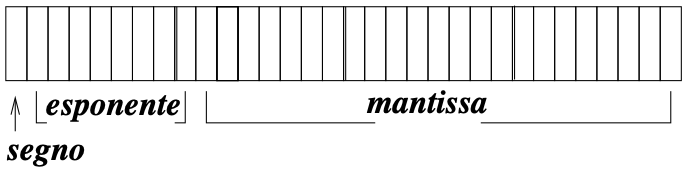
\includegraphics[width=0.5\linewidth]{images/IEEE.png}
    \centering
\end{figure}
\newpage
In precisione singola vengono destinati 24 bit alla mantissa (in realtà solo
23\footnote{Essendo sempre $\alpha_1$=1 per la rappresentazione binaria, la
prima cifra può essere sottintesa senza mai essere fisicamente memorizzata.}) e
8 all'esponente ($2^8=256=\omega-\lambda+1,\text{ con }\lambda=-127\text{ e
}\omega=128$), mentre in precisione doppia le cifre della mantissa sono 53
(memorizzati 52 bit) e dell'esponente 11 ($2^{11}=2048=\omega-\lambda+1,\text{
con }\lambda=-1023\text{ e }\omega=1024$).\\ 
Si osservi che l'esponente è memorizzato per traslazione (\textit{exponent
biased}) e che la costante di traslazione (\textit{bias}) è $-\lambda$. Quindi,
se $p$ è l'esponente del numero e $\tilde{p}$ è l'esponente memorizzato,
possiamo trovare l'esponente memorizzato a partire dall'esponente originale
utilizzando la seguente relazione:
$$\tilde{p}=p-\lambda$$
Dato un numero reale non nullo, $\alpha$, per associare un numero finito ad
esso, procediamo come segue:
\begin{enumerate}
    \item \textbf{Rappresentazione esatta}. Se $\alpha$ è scritto nella forma
        $\alpha=\pm(.\alpha_1\alpha_2\ldots)\times\beta^{p}$ tale che
        $\lambda\leq p\leq\omega$, $\alpha_i=0$ per $i> t$, allora è
        rappresentabile \underline{esattamente} come un numero finito $t$ di
        cifre e $\alpha\in \mathbb{F}(\beta,t,\lambda,\omega)$.
    \item \textbf{Rappresentazione approssimata}. Altrimenti 
        $\alpha\notin \mathbb{F}(\beta,t,\lambda,\omega)$ e quindi
        bisogna associargli un numero \underline{approssimato} $\tilde\alpha$
        che indicheremo con $fl(\alpha)$. Si hanno i seguenti casi:
        \begin{itemize}
            \item $p\notin[\lambda,\omega]$, viene segnalata una condizione
                d'errore:
                \begin{center}
                    \begin{tabular}{ll}
                        $p<\lambda$ & \textit{underflow} \\ 
                        $p>\lambda$ & \textit{overflow} \\ 
                   \end{tabular} 
                \end{center}
            \item $p\in[\lambda,\omega]$, ma le cifre $a_i$ con $i>t$ non sono
                tutte nulle, allora viene assegnato un numero finito $fl(\alpha)$
                seguendo due possibili criteri:
                \begin{itemize}
                    \item\textbf{Troncamento} di $\alpha$ alla t-esima cifra
                        $$fl_{T}(\alpha)=\pm(\sum_{i=1}^{t}\alpha_i\beta^{-i})\beta^p$$
                    \item\textbf{Arrotondamento} di $\alpha$ alla t-esima cifra 
                        $$fl_{A}(\alpha)=\pm
                        fl_{T}((\sum_{i=1}^{t+1}\alpha_i\beta^{-i}+\frac{\beta}{2}\beta^{-(t+1)})\beta^p)$$
                \end{itemize}
        \end{itemize}
\end{enumerate}
\begin{example}
    Il numero $\alpha=(0.11011)_2$ ha una mantissa di lunghezza 5, che è più
    lunga delle 3 cifre consentite in $\mathbb{F}(2,3,-1,2)$. Quindi, procediamo
    con l'operazione di arrotondamento:
    \begin{center}
       \begin{tabular}{lll}
           $fl_{A}(\alpha)=$ & $0.11011$ & + \\ 
                        & $0.00010$ & = \\ 
                        \hline
                        & $0.11100$ & \\ 
       \end{tabular} 
    \end{center}
\end{example}
\newpage
\begin{example}
   Consideriamo l'insieme dei numeri finiti $\mathbb{F}(10,5,-50,49)$. Per
   rappresentare un numero finito in questo insieme in memoria, dobbiamo
   definire il numero di posizioni necessarie. Nello specifico:
   \begin{itemize}
       \item\textbf{Segno}: una posizione è riservata per il segno. Se il numero
           è positivo si usa 0; se è negativo, si usa $\beta-1$.
        \item\textbf{Esponente}: due posizioni sono destinate all'esponente.
            Usando la tecnica di memorizzazione per traslazione
            ($p-\lambda=\tilde{p}$), possiamo
            rappresentare gli esponenti da -50 a 49 attraverso valori
            memorizzati da 00 a 99.
        \item\textbf{Mantissa}: cinque posizioni sono dedicate alla mantissa.
   \end{itemize}
   \begin{center}
        \begin{tabular}{ll}
            $\alpha=0.0532=0.532\cdot10^{-1}$ & $fl(\alpha)=04953200$\\ 
            $\alpha=-237141=-0.237141\cdot10^{6}$ & $fl(\alpha)=95623714$
        \end{tabular}
   \end{center}
\end{example}
\begin{oss}
    Siano $x$ ed $y$ due numeri $\in \mathbb{F}$ \underline{consecutivi}
    positivi. Sia $\alpha\in \mathbb{R}$ tale che $x\leq\alpha<y$. 
    \begin{center}
        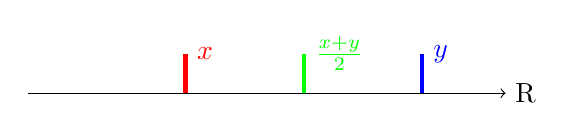
\begin{tikzpicture}
            \draw[->] (0,0) -- (0.5\linewidth,0) node[right] {R};

            \draw[red, ultra thick] (2,0) -- (2,0.5) node[right] {$x$};

            \draw[blue, ultra thick] (5,0) -- (5,0.5) node[right] {$y$};

            \draw[green, ultra thick] (3.5,0) -- (3.5,0.5) node[right] {$\frac{x+y}{2}$};
        \end{tikzpicture}
    \end{center}
    Allora possiamo affermare che $\alpha$ non appartiene all'insieme
    $\mathbb{F}$ perché, per ipotesi, $x$ e $y$ sono consecutivi e non ci può
    essere un altro numero tra loro. Tuttavia, la rappresentazione approssimata
    $fl(\alpha)$ risulta essere:
    \begin{center}
        \begin{tabular}{ll}
            $fl_T(\alpha)=x$ & $fl_A(\alpha)=\begin{cases}
                x & \text{se }\alpha<\frac{x+y}{2} \\ 
                y & \text{se }\alpha\geq \frac{x+y}{2}
            \end{cases}$
       \end{tabular} 
    \end{center}
    L'errore commesso nel troncamento sarà sempre maggiore o uguale dell'errore
    commesso nell'arrotondamento. Questo è il motivo per cui, con una base
    numerica pari, si preferisce utilizzare l'arrotondamento, poiché fornirà una
    migliore approssimazione del numero reale rispetto al troncamento.
\end{oss}
La modalità di arrotondamento dello standard ANSI/IEEE-754 coincide con quella
precedentemente descritta, con la particolarità dell'\textbf{arrotondamento ai
pari}. Questa particolarità si applica quando un numero reale $\alpha$ è esattamente 
equidistante dai numeri finiti consecutivi $x$ ed $y$, in altre parole, 
quando $\alpha=\frac{x+y}{2}$. In questa situazione l'arrotondamento funziona
nel seguente modo:
$$fl_{AP}(\alpha)=\begin{cases}
    x & \text{se }$x$\text{ è pari}\\ 
    $y$ & \text{se }$y$\text{ è pari}
\end{cases}$$
Sempre parlando dello standard ANSI/IEEE-754, per gestire risultati non rappresentabili, 
vengono utilizzati due valori speciali:
\begin{itemize}
    \item \textbf{NaN} 
    \item \textbf{Inf}
\end{itemize}
Invece, di avere un buco vicino allo zero dove i numeri molto piccoli
verrebbero immediatamente arrotondati a zero, vengono inseriti dei numeri ulteriori per
riempire questo vuoto e permettere ai valori di avvicinarsi progressivamente a zero.
Questo meccanismo è chiamato \textbf{gradual underflow}.\\ 
Per rappresentare questi numeri estremamente piccoli, si fa uso della
rappresentazione \textbf{denormalizzata}. In questa rappresentazione, la
mantissa  non inizia con il solito bit implicito di 1, ma  con una serie di 0.
\begin{example}
    Si eseguano i passi necessari per rappresentare il numero reale
    $(-13.9)_{10}$ in un'area di memoria di 8 bit (1 per il segno, 3 per
    l'exponent biased e 4 per la mantissa), che permettono di memorizzare
    $\mathbb{F}(2,5,-3,4)$ per troncamento e arrotondamento.
    \vskip 0.1in
    \begin{enumerate}
        \item \textbf{Conversione in binario}, prima la parte intera, quindi la parte decimale:
            \begin{itemize}
                \item \textit{Parte intera}:
                    \begin{enumerate}
                        \item Dividi il numero per 2.
                        \item Registra il resto della divisione (sarà 0 o 1).
                        \item Usa il quoziente ottenuto come nuovo numero e
                            ripeti la divisione per 2.
                        \item Continua il processo fino a quando il quoziente
                            diventa 0.
                        \item Leggi i resti della divisione in ordine
                            \underline{inverso}:
                            questo sarà il numero in base 2 della parte
                            intera.
                    \end{enumerate}
                    $$(13)_{10}=(1101)_2$$
                \item \textit{Parte decimale}:
                    \begin{enumerate}
                        \item Moltiplica la parte decimale per 2.
                        \item Registra la parte intera del risultato (sarà 0 o
                            1).
                        \item Usa la parte decimale del risultato come nuovo
                            numero e ripeti la moltiplicazione per 2.
                        \item Continua questo processo finché non ottieni una
                            parte decimale di 0 o si arriva al limite di
                            precisione della mantissa.
                        \item Leggi i numeri interi in ordine di apparizione:
                            questo sarà il numero in base 2 della parte
                            decimale.
                    \end{enumerate}
                    $$0.9\times2=\underline{1}.8$$
                    $$0.8\times2=\underline{1}.6$$
                    $$0.6\times2=\underline{1}.2$$
                    $$0.2\times2=\underline{0}.4$$
                    $$0.4\times2=\underline{0}.8$$
                    $$(0.9)_{10}=(11100\ldots)_2$$
            \end{itemize}
            da cui
            $$(-13.9)_{10}=(-1101.11100\ldots)_2$$
        \item \textbf{Normalizzazione}:
        nello standard IEEE-754, la rappresentazione normalizzata dei numeri
        in virgola mobile prevede che la parte \underline{intera} sia sempre
        1.
            $$(-1101.11100\ldots)_2=(-1.10111100\ldots)_2\times2^{3}$$
        \item \textbf{Calcolo dell'esponente biased}:
            $$p-\lambda=\tilde{p}\rightarrow3-(-3)=6$$
            $$(-1.10111100\ldots)_2\times2^3=(-1.10111100\ldots)_2\times2^{(110)_2}$$
        \item \textbf{Rappresentazione della mantissa}:
            \begin{center}
               \begin{tabular}{cc}
                    arrotondamento & troncamento \\ 
                   1.10111 + 0.00001 = 1.1100 & 1.1011
               \end{tabular} 
            \end{center}
        \item \textbf{Rappresentazione in memoria}: nello standard IEEE-754,
        con una mantissa di 5 bit, solo 4 bit vengono effettivamente memorizzati in memoria.
        \begin{center}
           \begin{tabular}{cc}
               $
               \begin{array}{|c|c|c|c|c|c|c|c|}
                   \hline
                   1 & 1 & 1 & 0 & 1 & 1 & 0 & 0\\
                   \hline
               \end{array} 
               $ 
                &
                $
                \begin{array}{|c|c|c|c|c|c|c|c|}
                    \hline
                    1 & 1 & 1 & 0 & 1 & 0 & 1 & 1 \\
                    \hline
                \end{array}
                $
           \end{tabular} 
        \end{center}
    \end{enumerate}
\end{example}
\subsection{Errori di rappresentazione}
\begin{definition}\leavevmode\
    Consideriamo un valore $\alpha\in \mathbb{R}$. Se $\alpha\notin
    \mathbb{F}(\beta,t,\lambda,\omega)$, allora la sua migliore
    approssimazione all'interno di questo insieme è data da $\tilde\alpha\in
    \mathbb{F}(\beta,t,\lambda,\omega)$. L'approssimazione di $\alpha$ con
    $\tilde\alpha$ introduce un \textbf{errore di rappresentazione}. Per quantificare
    tale errore, definiamo le seguenti metriche:
    {
        \renewcommand{\arraystretch}{1.5}
        \begin{center}
           \begin{tabular}{ll}
                $E_{abs}=\lvert \alpha-fl(\alpha)\rvert$ & errore assoluto \\
                $E_{rel}=\lvert \frac{\alpha-fl(\alpha)}{\alpha}\rvert\text{ se
            }\alpha\neq0$ & errore relativo 
           \end{tabular}
        \end{center}
    }
\end{definition}
Nel calcolo scientifico, l'errore relativo è preferito poiché fornisce una
misura dell'errore ``normalizzata'', che non dipende dalla grandezza dei numeri confrontati.
\begin{example}
    Si converta quanto rappresentato nell'esempio precedente nuovamente in
    base 10. Successivamente, si valuti l'errore assoluto e l'errore relativo
    della rappresentazione.
    \begin{enumerate}
        \setcounter{enumi}{5}
        \item\textbf{Decodifica}: per riconvertire il numero floating point
            appena determinato, faremo:
            \begin{center}
                 \begin{tabular}{ll}
                     arrotondamento & troncamento \\ 
                     $(-1.1100)_2\times2^{(110)_2}$ & $(-1.1011)_2\times2^{(110)_2}$ \\ 
                     $(-1.1100)_2\times2^{(3)_{10}}$ & $(-1.1011)_2\times2^{(3)_{10}}$ \\ 
                     $(-1110.0)_2$ & $(-1101.1)_2$ \\ 
                     $-(8+4+2+0+0)_{10}$ & $-(8+4+0+1+0.5)_{10}$ \\ 
                     $-(14)_{10}$ & $-(13.5)_{10}$ \\ 
                 \end{tabular}
            \end{center}
            \begin{center}
                \begin{tabular}{l|l|l}
                    & arrotondamento & troncamento \\
                    \hline
                    errore assoluto & $-13.9 - (-14) = 0.1$ & $-13.9 - (-13.5) = -0.4$ \\
                    \hline
                    errore relativo & $\frac{0.1}{-13.9} = -0.0072$ & $\frac{-0.4}{-13.9} = 0.0288$
                \end{tabular} 
            \end{center}
   \end{enumerate} 
\end{example}
\begin{definition}
    Dato l'insieme dei numeri finiti $\mathbb{F}(\beta,t,\lambda,\omega)$, si
    dice \textbf{unità di arrotondamento} e la si indica con $u$, la quantità:
    $$u=\begin{cases}
        \beta^{1-t} & \text{per troncamento} \\ 
        \frac{1}{2}\beta^{1-t} & \text{per arrotondamento}
    \end{cases}$$
\end{definition}
\begin{theorem}
   Per ogni $\alpha\in \mathbb{R}$ e $\alpha\notin0$ vale
   $$\Big\lvert \frac{\alpha-fl(\alpha)}{\alpha}\Big\rvert<u$$
\end{theorem}
Il teorema afferma che $u$, l'unità di arrotondamento, rappresenta il
\underline{limite superiore} dell'errore relativo quando si rappresenta 
un numero reale in un formato numerico finito.
\begin{example}
    Consideriamo l'insieme dei numeri finiti $\mathbb{F}(2,5,-3,4)$. Calcolare l'unità di arrotondamento $u$ sia nel caso di troncamento che di
    arrotondamento.
    $$u=\begin{cases}
        2^{1-5}=\frac{1}{16}=0.0625 & \text{per
        troncamento} \\
        \frac{1}{2}\cdot2^{1-5}=\frac{1}{32}=0.0325 & \text{per arrotondamento}
    \end{cases}$$
\end{example}
Indicheremo con $\epsilon$ l'errore relativo.
\begin{corollary}
    Per ogni $\alpha\in \mathbb{R}$ e $\alpha\notin0$ vale 
    $$  fl(\alpha)=\alpha(1\pm\epsilon),\quad \text{con }\lvert 
      \epsilon\rvert<u $$
\end{corollary} 
\begin{proof}\leavevmode\\
    Banalmente dato $\epsilon=\frac{\alpha-fl(\alpha)}{\alpha}$,
    per il Teorema si ha che $\lvert \epsilon\rvert<u$ e
    $fl(\alpha)=\alpha\epsilon+\alpha=\alpha(1+\epsilon)$.
\end{proof}
\paragraph{Precisione desiderata in base 10.}
La questione chiave è: quante cifre in base 10 sono necessarie per
rappresentare con precisione ciò che è memorizzato in base 2? 

Supponiamo di avere un numero rappresentato con $t$ cifre in base 2. Vogliamo
sapere a quante cifre, $s$, in base 10 questo corrisponde.

Partendo dall'equazione:
$$2^{-t}=10^{-s}$$
e applicando il logaritmo in base 10 ad entrambi i lati:
$$-t\times\log_{10}(2)=-s$$
da qui possiamo isolare $s$:
$$s=t\times\log_{10}(2)$$
usando un'approssimazione per il logaritmo:
$$s \approx t \times 0.30103$$

Per esempio:
\begin{itemize}
\item Nella precisione `basic single', con \( t = 24 \) cifre in base 2 per la mantissa, abbiamo:
$$s \approx 24 \times 0.30103 \approx 7.224$$
\item Nella precisione `basic double', con \( t = 53 \) cifre in base 2 per la mantissa, abbiamo:
$$s \approx 53 \times 0.30103 \approx 15.95459$$
\end{itemize}
Questo indica che ci servono circa 7-8 cifre in `basic single' o circa 16
cifre in `basic double' in base 10 per rappresentare con
precisione ciò che è memorizzato in base 2. Utilizzando meno cifre, stiamo
arrotondando e potremmo perdere informazioni.

Possiamo calcolare l'unità di arrotondamento $u$ per `basic single' e `basic
double':
\begin{itemize}
    \item $u_{single}= \frac{1}{2} \times 2^{1-24}=2^-24\approx 5.96 \times
        10 ^{-8}$ 
    \item $u_{double}= \frac{1}{2} \times 2^{1-53}=2^-53\approx 1.116 \times
        10 ^{-16}$ 
\end{itemize}
Ora, se confrontiamo questi valori con le cifre necessarie in base 10 per
una rappresentazione accurata, notiamo una relazione. Le cifre necessarie
sono legate all'ordine di grandezza dell'unità di arrotondamento.

Questi valori forniscono un indicatore sull'ordine di grandezza minimo dei 
numeri che possono essere rappresentati accuratamente e sul numero massimo di 
cifre che possiamo stampare senza perdere informazioni.
\subsection{Aritmetica finita}
Dati due numeri $a$ e $b$ appartenenti a $\mathbb{F}(\beta,t,\lambda,\omega)$,
l'operazione $a\ op\ b$ potrebbe produrre un risultato che non è contenuto in
$\mathbb{F}(\beta,t,\lambda,\omega)$.
\begin{example}
    Siano $a=(0.34)_{10}\times10^{0}$ e $b=(0.12)_{10}\times10^{-2}\in
    \mathbb{F}(10,2,\lambda,\omega)$. Eseguendo la somma si ha: 
    $$0.34+0.0012=0.3412$$
    ma, $0.3412\notin \mathbb{F}(10,2,\lambda,\omega)$.
\end{example}
Per eseguire le operazioni in questo dominio, vengono definiti degli
operatori specifici, che indichiamo con $\tilde{op}$ (ad esempio, $\tilde{+},
\tilde{-}, \tilde{*}, \tilde{/}$).
\begin{definition}
    L'operatore $\tilde{op}$ tra due numeri $a,b\in \mathbb{F}$ è definito nel modo seguente:
    $$a\ \tilde{op}\ b=fl(a\ op\ b)$$
    Questo significa che viene prima eseguita l'operazione in aritmetica
    esatta, e il risultato viene arrotondato per rientrare nell'insieme di
    numeri finiti $\mathbb{F}$.
\end{definition}
Per soddisfare tali requisiti, si utilizzano dei registri posizionati vicino 
al processore. Questi registri, dotati di bit aggiuntivi, 
rispetto a quelli della mantissa, permettono di eseguire operazioni con una
precisione superiore rispetto a quella raggiungibile con solo $t$ bit. Tale
maggiore precisione assicura che, arrotondando a $t$ cifre, il risultato ottenuto
aderisce alla definizione delineata sopra. Idealmente, un registro di lunghezza
$t+1$ bit, superiore a quella della mantissa stessa, garantirebbe la
conformità a questa definizione.
\vskip 0.1in
\paragraph{Errore in aritmetica finita.}
Qual'è l'errore massimo che possiamo commettere durante un operazione con numeri
finiti?
Consideriamo l'errore relativo tra il risultato ottenuto in aritmetica finita
e quello in aritmetica esatta, si può notare un interessante comportamento. 
Notiamo che, il risultato esatto di $(a\ op\ b)$ è un numero $\alpha\in
\mathbb{R}$. Per definizione, in aritmetica finita, $(a\ \tilde{op}\ b)$ è
l'approssimazione floating-point di $\alpha$.
Allora, per il teorema sopra menzionato, possiamo dedurre che l'errore relativo massimo tra
$\alpha$ e $fl(\alpha)$ è minore dell'unità di arrotondamento $u$. Questo
significa che $u$ rappresenta l'errore relativo massimo che possiamo
aspettarci in una singola operazione in aritmetica finita.
Estendendo questa logica, se effettuiamo una serie di $n$ operazioni, l'errore
totale potrebbe essere al più $n\cdot u$.
$$\Big\lvert \frac{\overset{fl(\alpha)}{\overbrace{(a\ \tilde{op}\ b)}}-\overset{\alpha}{\overbrace{(a\ op\
b)}}}{\underset{\alpha}{\underbrace{a\ op\ b}}}\Big\rvert<u$$
\paragraph{Proprietà associativa.} La proprietà associativa afferma che
l'ordine in cui si raggruppano i termini durante un'operazione non modifica il
risultato. Tuttavia, essa, così come le altre proprietà, \underline{non} vale nell'aritmetica finita.
\begin{example}
    Considerati $a=0.11\times10^0,b=0.13\times10^{-1},c=0.14\times10^{-1}\in
    \mathbb{F}(10,2,\lambda,\omega)$.
    Verificare se la proprietà associativa
    $(a\tilde+b)\tilde+c=a\tilde+(b\tilde+c)$ è valida.
    \begin{equation*}
        \begin{aligned}
            (0.11\tilde+0.013)\tilde+0.014&=0.11\tilde+(0.013\tilde+0.014) \\ 
            fl(0.123)\tilde+0.014&=0.11\tilde+fl(0.027)\\ 
            0.12\tilde+0.014&=0.11\tilde+0.03 \\ 
            fl(0.134)&=0.14 \\
            0.13\times10^0&\neq0.14\times10^0
        \end{aligned} 
    \end{equation*}
    Concludendo, la proprietà associativa non è valida nell'ambito dell'aritmetica finita.
\end{example}
Questo significa che la stessa istruzione o espressione, se scritta in modi
diversi, può produrre risultati differenti. 
Di conseguenza, è importante comprendere come evitare di scrivere operazioni che
potrebbero causare errori più grandi.
\subsubsection{Caratterizzazione di $u$}
L'unità di arrotondamento $u$ ha un'importanza numerica sia in relazione alla precisione
di rappresentazione (Teorema) che in termini di precisione di calcolo (risultato precedente).
La sua importanza numerica è ulteriormente sottolineata dalla seguente
caratterizzazione:

\begin{center}
    \emph{$u$ è il più piccolo numero finito positivo tale che, se sommato a
    1, viene ``sentito'' e risulta essere $>$ di 1.}
\end{center}
$$u\tilde+1>1$$
Questo implica che per ogni numero finito $v<u$ sarà $v\tilde+1=1$.

Infatti, se sommiamo un numero $v$ a $1$:
    $$
    \underbrace{1.0 \ldots 0}_{t \text{ cifre}} + \underbrace{0.0 \ldots 0}_{t
    \text{ cifre}}1
    $$
Tuttavia, il valore $1$ rimane fuori dalle $t$ cifre e nella somma viene
arrotondato, e non viene ``sentito'' poiché il risultato sarà comunque $1$.

\begin{center}
    \begin{tikzpicture}
        \draw[->] (-2,0) -- (2*5,0) node[right] {R};
        \draw (0,0.1) -- (0,-0.1) node[below] {0};
        \draw[blue] (1,0) -- (1,-0.4) node[below] {$u\tilde+1>1$};
        \draw[red] (1,0) -- (1,0.4) node[above] {$v\tilde+1$=1};
        \draw[blue] (1,-0.4) -- (2*3.5,-0.4);
        \draw[red] (1,0.4) -- (0,0.4);
        \draw[dashed, blue] (2*3.5,-0.4) -- (2*4,-0.4);
        \filldraw (0,0) circle (0.05);

        \foreach \x in {0.25, 0.3125, 0.375, 0.4375, 0.625, 0.75, 0.875, 1, 1.25, 1.5, 1.75, 2, 2.5, 3, 3.5} {
            \draw (2*\x,-0.1) -- (2*\x,0.1);
        }
    \end{tikzpicture}
\end{center}
Invece, se sommiamo un numero $u$ a 1:
\begin{equation*}
   \begin{aligned}
       u\tilde+1&=\frac{1}{2}\beta^{1-t}+1 \\ 
                &=\frac{\beta}{2}\beta^{-t}+1 \\
                &=0.0\ldots0\frac{\beta}{2}+\underbrace{1.0\ldots0}_{t\text{
                cifre}} \\ 
                &= 1.0\ldots0 \frac{\beta}{2}+0.0+0.0\ldots0 \frac{\beta}{2}
                \text{ per arrotondamento}\\
                &= \underbrace{1.0\ldots1}_{t\text{ cifre}}0 \text{ per
                troncamento}\\
                1.0\ldots1&>1
   \end{aligned} 
\end{equation*}
Nello standard IEEE-754, se consideriamo l'arrotondamento ai pari e dato che
$1.0\ldots0 \frac{\beta}{2}=\frac{x+y}{2}$, dove $x=1$ e
$y=1.0\ldots1$, il valore pari più vicino è 1. Pertanto, 1 verrà scelto come
risultato dell'arrotondamento. Questo cambia la caratterizzazione di $u$:
\begin{center}
    \emph{$u$ è il più grande numero finito positivo tale che, se sommato a 1,
    risulta essere $=1$}.
\end{center}
$$u\tilde+1=1$$
\begin{center}
    \begin{tikzpicture}
        \draw[->] (-2,0) -- (2*5,0) node[right] {R};
        \draw (0,0.1) -- (0,-0.1) node[below] {0};
        \draw[red] (1,0) -- (1,-0.4) node[below] {$v\tilde+1>1$};
        \draw[blue] (1,0) -- (1,0.4) node[above] {$u\tilde+1$=1};
        \draw[red] (1,-0.4) -- (2*3.5,-0.4);
        \draw[blue] (1,0.4) -- (0,0.4);
        \draw[dashed, red] (2*3.5,-0.4) -- (2*4,-0.4);
        \filldraw (0,0) circle (0.05);

        \foreach \x in {0.25, 0.3125, 0.375, 0.4375, 0.625, 0.75, 0.875, 1, 1.25, 1.5, 1.75, 2, 2.5, 3, 3.5} {
            \draw (2*\x,-0.1) -- (2*\x,0.1);
        }
    \end{tikzpicture}
\end{center}
Ma cosa ci serve tutto a questo? Per determinare proceduralmente $u$:
\begin{enumerate}
    \item Esaminare le potenze negative di 2.
    \item Continuare finché non si individua una potenza $2^{-t}$ che, quando sommata a 1,
        produce come risultato esattamente 1.
    \item Tale potenza $2^{-t}$ rappresenta l'unità di arrotondamento $u$.
\end{enumerate}
\begin{verbatim}
    u=1
    t=0
    while (u+1>1)
        u=u/2
        t=t+1
    end 
    stampa(u,t)
\end{verbatim}
\subsection{Analisi degli errori}
Nella risoluzione di problemi in aritmetica finita su un calcolatore, dobbiamo
prima chiederci cosa sia un ``problema ben posto''. Per definire un problema come 
\textbf{ben posto}, è necessario che soddisfi due requisiti:
\begin{itemize}
    \item Il problema deve ammettere una e
        una sola soluzione.
    \item La soluzione deve dipendere con
        continuità dai dati in ingresso.
\end{itemize}
Un buon modo per \underline{modelizzare} il nostro problema è tramite una funzione 
$f:\mathbb{R}\rightarrow \mathbb{R}$ che a partire da un dato $x$ produce un
risultato $f(x)$. Affinché il problema sia ben
posto, questa funziona deve essere continua. E per la sua stessa
definizione, una funzione restituisce sempre un unico output per ogni input.

Ora, consideriamo un tipico flusso di lavoro legato alla risoluzione di un
problema su un calcolatore:
\begin{itemize}
    \item \textbf{Input}. Il dato viene letto e tradotto in
        una rappresentazione in aritmetica finita.
    \item \textbf{Elaborazione}. Si applica un algoritmo, anch'esso in aritmetica
    finita, per elaborare il dato.
    \item \textbf{Valutazione del risultato}. Si esamina il risultato,
        l'errore associato e si decide se il risultato è
        accettabile oppure no.
\end{itemize}
Per valutare l'entità dell'errore, possiamo utilizzare:
\begin{itemize}
    \item\textbf{Analisi in avanti}: si calcola l'errore relativo sul
        risultato finale in termini degli errori introdotti dalle singole
        operazioni, trascurando i termini in cui compaiono prodotti di errori
        (analisi del $1^{\circ}$ ordine).
    \item\textbf{Analisi all'indietro}: approccio opposto al precedente
        consiste nel considerare il risultato $\tilde{f}(x+\delta x)$ come risultato 
        esatto derivato da dati iniziali perturbati rispetto a quelli reali.
        La valutazione è data quindi da un fattore
        $\delta x$ sul dato iniziale $x$.
\end{itemize}
\begin{figure}
    \centering
    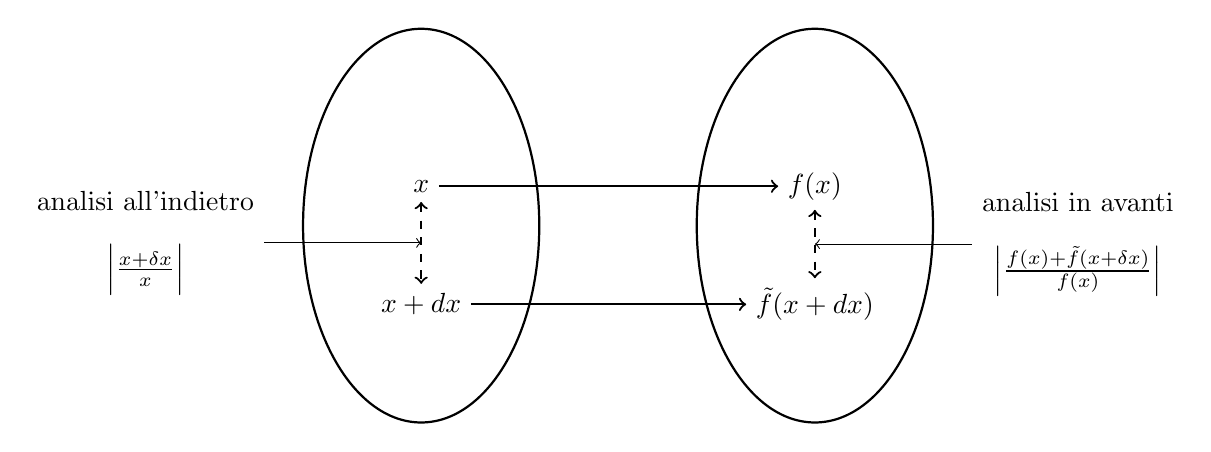
\begin{tikzpicture}
        \draw[thick] (0,2.5) ellipse (1.5cm and 2.5cm);
        \draw[thick] (5,2.5) ellipse (1.5cm and 2.5cm);
        
        \node (x) at (0,3) {$x$};
        \node (xdx) at (0,1.5) {$x+dx$};
        \node (fx) at (5,3) {$f(x)$};
        \node (fdx) at (5,1.5) {$\tilde{f}(x+dx)$};
        
        \draw[->, thick] (x) -- (fx);
        \draw[->, thick] (xdx) -- (fdx);
        
        \draw[<->, dashed, thick] (x) -- (xdx) coordinate[midway] (m1);
        \draw[<->, dashed, thick] (fx) -- (fdx) coordinate[midway] (m2);

        \draw[<-] (m1) -- ++(-2,0) node[left, align=center] {analisi
            all'indietro\\\\$\Big\lvert \frac{x+\delta x}{x}\Big\rvert$};
        \draw[<-] (m2) -- ++(2,0) node[right, align=center] {analisi in
                avanti\\\\$\Big\lvert
        \frac{f(x)+\tilde{f}(x+\delta x)}{f(x)}\Big\rvert$};
\end{tikzpicture}
\caption{Analisi dell'errore}
\label{fig:analisi_errore}
\end{figure}
L'immagine \ref{fig:analisi_errore} mostra che se la distanza tra $x$ e
$x+\delta x$ è piccola e, analogamente, la distanza tra $f(x)$ e
$\tilde{f}(x+\delta x)$ è anch'essa piccola, allora possiamo considerare il
risultato come ``buono''.
\subsubsection{Analisi in avanti degli errori nelle operazioni di moltiplicazione e addizione}
Applicando l'analisi in avanti alle operazioni di moltiplicazione e addizione
si ottengono alcuni importanti risultati:
\begin{itemize}
    \item \textbf{Moltiplicazione}: 
        Siano $x,y\in \mathbb{R}$. Consideriamo la funzione $f:\mathbb{R}^2\rightarrow
        \mathbb{R}$  definita come $f(x,y)=x\cdot y$, che moltiplica due numeri
        reali e restituisce il risultato. 

        Applichiamo l'analisi in avanti, 
        tenendo conto sia dell'errore sui dati che dell'errore di calcolo:
        \begin{equation*}
           \begin{aligned}
                x \rightarrow fl(x)&=x(1+\epsilon_1) & \lvert \epsilon_1\rvert <
               u\\
                y\rightarrow fl(y)&=y(1+\epsilon_2) & \lvert
                \epsilon_2\rvert< u\\
                 fl(x)\cdot fl(y)&=fl(fl(x)fl(y))\\ 
                                 &=fl(x)fl(y)(1+\epsilon_3) &
                                 \lvert \epsilon_3\rvert<u\\ 
                                 &= x(1+\epsilon_1)
                                 y(1+\epsilon_2)(1+\epsilon_3)
           \end{aligned} 
        \end{equation*}

        Calcoliamo ora l'errore relativo:
        \begin{equation*}
           \begin{aligned}
                \Big\lvert \frac{fl(fl(x)
                fl(y))-f(x,y)}{f(x,y)}\Big\rvert &= \Big\lvert
                \frac{x(1+\epsilon_1)y(1+\epsilon_2)(1+\epsilon_3)-xy}{xy}\Big\rvert
                \\ 
                &= \Big\lvert
                \frac{\cancel{(xy)}((1+\epsilon_1)(1+\epsilon_2)(1+\epsilon_3)-1)}{\cancel{xy}}\Big\rvert
                \\ 
                &= \Big\lvert
                (1+\epsilon_1)(1+\epsilon_2)(1+\epsilon_3)-1\Big\rvert\\ 
                &= \Big\lvert \cancel{1}+
                \epsilon_1+\epsilon_2+\epsilon_3+\epsilon_1\epsilon_2+\epsilon_1\epsilon_3+\epsilon_2\epsilon_3+\epsilon_1\epsilon_2\epsilon_3-\cancel{1}\Big\rvert
           \end{aligned} 
        \end{equation*}

        Trascuriamo il prodotto di errori, poiché numericamente irrilevanti
        (analisi di $1^{\circ}$ ordine):
        $$\approx \lvert \epsilon_1+\epsilon_2+\epsilon_3\rvert \leq \lvert
        \epsilon_1\rvert+\lvert \epsilon_2\rvert+\lvert \epsilon_3\rvert<3u$$

        Abbiamo quantificato un limite superiore per l'errore sul risultato
        finale. Dato che ci sono 3 operazioni e l'errore finale massimo è di
        $3u$, il risultato è sia accettabile che aspettato.
    \item \textbf{Addizione}:
        Siano dati $x,y\in \mathbb{R}$. Consideriamo la funzione $f:
        \mathbb{R}^2\in \mathbb{R}$ definita come $f(x,y)=x+y$, che somma due
        numeri reali e restituisce il risultato.

        Applichiamo l'analisi in avanti, tenendo conto sia dell'errore sui dati che dell'errore di calcolo:
        \begin{equation*}
           \begin{aligned}
                x \rightarrow fl(x) &= x(1+\epsilon_1) & |\epsilon_1| < u \\
                y \rightarrow fl(y) &= y(1+\epsilon_2) & |\epsilon_2| < u \\
                fl(x) + fl(y) &= fl(fl(x)+fl(y)) \\
                              &= (fl(x)fl(y))(1+\epsilon_3) & |\epsilon_3| < u \\
                              &= (x(1+\epsilon_1) + y(1+\epsilon_2))(1+\epsilon_3)
           \end{aligned} 
        \end{equation*}

        Calcoliamo ora l'errore relativo:
        \begin{equation*}
           \begin{aligned}
                \Big\lvert \frac{fl(fl(x) + fl(y)) - f(x,y)}{f(x,y)}
                \Big\rvert &= \Big\lvert \frac{(x(1+\epsilon_1) +
                y(1+\epsilon_2))(1+\epsilon_3) - (x + y)}{x + y} \Big\rvert \\
                &= \Big\lvert
                \frac{(x+y+x\epsilon_1+y\epsilon_2)(1+\epsilon_3)-(x+y)}{x + y} \Big\rvert \\
                &= \Big\lvert
                \frac{\cancel{(x+y)}+x\epsilon_1+y\epsilon_2+x\epsilon_3+y\epsilon_3+x\epsilon_1\epsilon_3+y\epsilon_2\epsilon_3-\cancel{(x+y)}}{x+y}\Big\rvert
           \end{aligned} 
        \end{equation*}
        
        Trascuriamo il prodotto di errori, poiché numericamente irrilevanti
        (analisi del $1^{\circ}$ ordine):
        $$\approx \Big\lvert
        \frac{x}{x+y}\epsilon_1+\frac{y}{x+y}\epsilon_2+\frac{x+y}{x+y}\epsilon_3\Big\rvert\leq
        \Big\lvert \frac{x}{x+y}\Big\rvert\lvert \epsilon_1\rvert+\Big\lvert
        \frac{y}{x+y}\Big\rvert \lvert \epsilon_2\rvert+\lvert
        \epsilon_3\rvert\nless 3u$$

        Che cosa è successo? Non possiamo dire che l'errore sia sempre $<3u$.
        Infatti, i fattori $\frac{x}{x+y}$ e $\frac{y}{x+y}$ agiscono come
        amplificatori degli errori $\epsilon_1$ e $\epsilon_2$. Ma quando questi fattori diventano grandi?
        Quando $x,y\in \mathbb{R}$ sono di segno opposto e con valori quasi
        uguali. 

        Questo fenomeno è conosciuto come \textbf{errore di
        cancellazione numerica}. Si tratta di una perdita di
        precisione durante operazioni di addizione o sottrazione. Esso si
        verifica quando:
        \begin{itemize}
            \item $x$ e $y$ sono di segno opposto e con valori quasi uguali;
            \item vi è un errore $\epsilon_1$ nella rappresentazione di $x$ o
                un errore $\epsilon_2$ in quella di $y$.
        \end{itemize}
        Anche se questi fattori fossero grandi, in assenza degli
        errori $\epsilon_1$ o $\epsilon_2$, non avremmo un amplificazione
        dell'errore. Tuttavia, è proprio la presenza di errori nella
        rappresentazione, unita ai fattori di amplificazione, che può
        rendere il risultato finale meno preciso di quanto ci si potrebbe
        aspettare.
\end{itemize}
\begin{example}
   Sia $\mathbb{F}(10,6,\lambda,\omega)$ con rappresentazione per arrotondamento e siano
   dati i numeri reali $\alpha=0.147554326$ e $b=-0.147251742$. 

   La loro approssimazione nell'insieme $\mathbb{F}$ sarà:
   $fl(a)=0.1475543+0.0000005=0.147554$ e
   $fl(b)=0.1472517+0.0000005=0.147252$.

   L'addizione esatta darà: $a+b=0.302584\times10^{-3}$, mentre in aritmetica
   finita darà:
   $fl(fl(a)+fl(b))=fl(0.147554-0.147252)=0.000302=0.302000\times10^{-3}$.

   L'errore relativo commesso sarà:
   $\frac{0.302000\times10^{-3}-0.302584\times10^{-3}}{0.302584\times10^{-3}}\approx0.2\times10^{-2}$,
   mentre $u=\frac{1}{2}10^{1-6}=0.5\times10^{-5}$ comportando un grave
   errore.

   Nel cancellare delle cifre a causa dell'arrotondamento, ho perso
   delle informazioni successive. Questa perdita si traduce in un errore che è
   maggiorato di ben tre ordini di grandezza. 
\end{example}
\subsubsection{Condizionamento di un problema e stabilità di un algoritmo}

Ci interessa comprendere dell'errore totale, quanto di
quest'ultimo sia risultato dall'approssimazione dei dati e quanto invece sia
dovuto all'algoritmo che stiamo utilizzando.

Iniziamo dividendo l'errore totale in due componenti:
\begin{itemize}
    \item \textbf{Condizionamento del problema}: Questo rappresenta l'errore
        che è intrinsecamente associato ai dati di input del problema. In altre
        parole, è l'errore che non possiamo eliminare in quanto è legato alla
        qualità dei dati stessi. Possiamo chiamarlo \textbf{errore inerente}.
        Per quantificarlo, prendiamo il dato reale, lo approssimiamo e poi
        valutiamo l'errore relativo tra il risultato ottenuto in aritmetica esatta  
        utilizzando il  dato approssimato e quello che avremmo ottenuto utilizzando il dato
        vero.
        $$E_{in}=\Big\lvert \frac{f(\tilde{x})-f(x)}{f(x)}\Big\rvert$$
    \item \textbf{Stabilità dell'algoritmo}: Questo rappresenta l'errore
        introdotto dall'algoritmo che stiamo utilizzando per risolvere il
        problema. È il contributo dell'algoritmo nell'amplificare gli errori
        presenti nei dati. Possiamo chiamarlo \textbf{errore algoritmico}. Per
        valutarlo, confrontiamo il risultato finale ottenuto utilizzando
        l'algoritmo in aritmetica finita con il risultato teorico che
        l'algoritmo avrebbero fornito operando in aritmetica esatta,
        considerando che dati iniziali siano già stati approssimati.
        $$E_{alg}=\Big\lvert
        \frac{\tilde{f}(\tilde{x})-f(\tilde{x})}{f(\tilde{x})} \Big\rvert$$
\end{itemize}
\begin{theorem}
    Siano $x$ e $\tilde{x}$ tale che $f(x)\neq0$ ed $f(\tilde{x})\neq0$.
    Indicati con $E_{tot}=\Big\lvert
    \frac{\tilde{f}(\tilde{x})-f(x)}{f(x)}\Big\rvert$ l'errore relativo 
    nell'analisi in avanti e con
    $E_{in}$ ed $E_{alg}$ gli errori inerente e algoritmo, si ha 
    \begin{equation} \label{eq:2}
        E_{tot}=E_{alg}(1+E_{in})+E_{in}
    \end{equation}
    Trascurando il prodotto di errori, la \ref{eq:2} risulta così semplificata:
    {\color{green}$$E_{tot}\approx E_{alg}+E_{in}$$}
\end{theorem}

Un problema è definito come mal condizionato quando presenta un elevato errore inerente.
Al contrario, quando l'errore inerente è ridotto, il problema è definito come ben condizionato. 
D'altro canto, se un algoritmo produce un ampio errore algoritmico, viene
definito instabile.
Se, invece, l'errore algoritmico è minimo, l'algoritmo è definito come numericamente stabile.

\begin{example}
    Calcolare gli errori inerente e algoritmico associati all'addizione di
    $x+y$, dove $x,y\in \mathbb{R}$.
    \begin{equation*}
        \begin{aligned}
            \tilde{x}=fl(x) &= x(1+\epsilon_1) & |\epsilon_1| < u \\
            \tilde{y}=fl(y) &= y(1+\epsilon_2) & |\epsilon_2| < u \\
        \end{aligned} 
     \end{equation*}
    \begin{equation*}
       \begin{aligned}
           E_{in}&= \Big\lvert \frac{f(\tilde{x},\tilde{y})-f(x,y))}{f(x,y)}\Big\rvert\\
            &=\Big\lvert
           \frac{x(1+\epsilon_1)+y(1+\epsilon_2)-(x+y)}{x+y}\Big\rvert \\
                 &=\Big\lvert
                     \frac{\cancel{(x+y)}+x\epsilon_1+y\epsilon_2-\cancel{(x+y)}}{x+y}
                    \big\rvert \\ 
                &=\Big\lvert
                \frac{x}{x+y}\epsilon_1+\frac{y}{x+y}\epsilon_2\Big\rvert\\ 
                &\leq \Big\lvert \frac{x}{x+y}\Big\rvert \lvert
                \epsilon_1\rvert + \Big\lvert \frac{y}{x+y}\Big\rvert \lvert
                \epsilon_2\rvert\\
           E_{alg}&=\Big\lvert
           \frac{\tilde{f}(\tilde{x},\tilde{y})-f(\tilde{x},\tilde{y})}{f(\tilde{x},\tilde{y})}\Big\rvert
           \\ 
                &= \Big\lvert
                \frac{(\tilde{x}+\tilde{y})(1+\epsilon_3)-(\tilde{x}+\tilde{y})}{\tilde{x}+\tilde{y}}\Big\rvert\\
                &= \lvert \epsilon_3\rvert
       \end{aligned} 
    \end{equation*}
\end{example}
\begin{example}
   Si analizzi il condizionamento e la stabilità dell'algoritmo utilizzato calcolare la funzione $f:\mathbb{R}\rightarrow
   \mathbb{R}$ definita come $f(x)=\frac{(1+x)-1}{x}$ e dove $x\in
   \mathbb{F}\subset \mathbb{R}\text{ e }x\neq0$.
   \begin{equation*}
        \begin{aligned}
           \tilde{x}&=fl(x)=x(1+\epsilon_1) & \lvert\epsilon_1\rvert < u \\
           E_{in}&=\Big\lvert \frac{f(\tilde{x})-f(x)}{f(x)}\Big\rvert\\ 
                 &=\Big\lvert
                 \frac{(1+x(1+\epsilon_1))-1}{x(1+\epsilon_1)}-1\Big\rvert\\ 
                 &=0
       \end{aligned} 
   \end{equation*}
    
   Le operazioni principali e i loro errori associati sono:
   \begin{itemize}
        \item un'addizione con errore $\epsilon_1$,
        \item una sottrazione con errore $\epsilon_2$, e
        \item una divisione con errore $\epsilon_3$.
   \end{itemize}

   \begin{equation*}
       \begin{aligned}
           E_{alg}&=\Big\lvert\frac{\tilde{f}(\tilde{x})-f(\tilde{x})}{f(\tilde{x})}\Big\rvert\\ 
                  &=\Big\lvert
                  \frac{\frac{((1+x)(1+\epsilon_1)-1)(1+\epsilon_2)}{x}(1+\epsilon_3)-1}{1}\Big\rvert\\ 
                  &=\Big\lvert
                  \frac{\cancel{1}+x+(1+x)\epsilon_1-\cancel{1}}{x}(1+\epsilon_2)(1+\epsilon_3)-1\Big\rvert\\ 
                  &=\Big\lvert
                  \frac{x(1+\epsilon_2)(1+\epsilon_3)+(1+x)\epsilon_1(1+\epsilon_2)(1+\epsilon_3)}{x}-1\Big\rvert\\ 
                  &=\Big\lvert
                  \cancel{1}+\epsilon_2+\epsilon_3+\epsilon_2\epsilon_3+\frac{1+x}{x}\epsilon_1(1+\epsilon_2+\epsilon_3+\epsilon_2\epsilon_3)-\cancel{1}\Big\rvert
       \end{aligned}
   \end{equation*}
   Trascurando il prodotto di errori, poiché numericamente irrilevanti
   (analisi di $1^{\circ}$ ordine):
   $$\approx \frac{1+x}{x}\epsilon_1+\epsilon_2+\epsilon_3$$
   $$\frac{1}{x}\epsilon_1+\epsilon_1+\epsilon_2+\epsilon_3\leq \Big\lvert
   \frac{1}{x}\Big\rvert \lvert \epsilon_1\rvert + \underbrace{\lvert \epsilon_1\rvert +
\lvert \epsilon_2\rvert + \lvert \epsilon_3\rvert}_{3u}$$
    Come interpretare questo risultato finale? Su quest'ultimo può esserci un
    errore $>3u$. Se l'errore $\epsilon_1$ nella prima addizione è $\neq0$ e
    $x$ è piccolo, il termine $\frac{1}{x}$ diventa grande, amplificando così
    l'errore.
\end{example}

\subsubsection{Numero di condizione}
\paragraph{Funzioni $f:\mathbb{R}\rightarrow \mathbb{R}$.}
Consideriamo una funzione $f:\mathbb{R}\rightarrow \mathbb{R}$ che sia
\underline{differenziabile}. Supponendo che vogliamo valutare questa funzione in un
punto vicino a $x_0$, possiamo usare lo sviluppo di Taylor centrato in
$x_0$:

$$f(x)=f(x_0)+f'(x_0)(x-x_0)+o(h)$$
dove $h=x-x_0$.

Se vogliamo approssimare $f$ in un punto vicino $x_0$, diciamo
$\tilde{x}_0$ abbiamo:

$$f(\tilde{x}_0)=f(x_0)+f'(x_0)(\tilde{x}_0-x_0)+o(h)$$

Calcoliamo l'errore inerente:
\begin{equation*}
    \begin{aligned}
        E_{in}&= \Big\lvert \frac{f(\tilde{x}_0)-f(x_0)}{f(x_0)}\Big\rvert \\
            \alignedintertext{Sostituendo lo sviluppo di Taylor per
            $f(\tilde{x}_0)$, possiamo riscrivere:}
            &\approx \Big\lvert
            \frac{\cancel{f(x_0)}+f'(x_0)(\tilde{x}_0-x_0)-\cancel{f(x_0)}}{f(x_0)}\Big\rvert\\
            &=\Big\lvert
            \frac{f'(x_0)(\tilde{x}_0-x_0)}{f(x_0)}\cdot \frac{x_0}{x_0}\Big\rvert & \text{per ipotesi }
            f(x_0)\neq0 \text{ e }x_0\neq0\\ 
            &= \Big\lvert
            \frac{f'(x_0)x_0}{f(x_0)}\frac{\tilde{x}_0-x_0}{x_0}\Big\rvert\\ 
            \alignedintertext{Se si considera
            $\frac{\tilde{x}_0-x_0}{x_0}$ come 
            l'errore sui dati, possiamo riscrivere:}
            &= {\color{red}\Big\lvert \frac{f'(x_0)x_0}{f(x_0)}\Big\rvert} \lvert
            \epsilon_{x_0}\rvert
    \end{aligned}
\end{equation*}

Ciò che emerge è che l'errore inerente non dipende soltanto dall'errore sui
dati, ma anche da una quantità $\Big\lvert \frac{f'(x_0)x_0}{f(x_0)}\Big\rvert$ che amplifica tale errore.
Questa quantità è nota come \textbf{numero di condizione} e lo denotiamo con
$C(f, x_0)$. 

Un valore elevato di $C(f, x_0)$ indica che il problema è mal condizionato in
$x_0$, cioè piccoli errori nei dati possono portare a grandi errori nella
soluzione.

Pertanto, per determinare se un problema differenziabile è mal condizionato in
un dato punto, si può guardare il suo numero di condizione.

\paragraph{Generalizzazione per funzioni $f:\mathbb{R}^n\rightarrow
\mathbb{R}$.} Dati una funzione $f:\mathbb{R}^n\rightarrow \mathbb{R}$ e due
vettori $x=(x_1,x_2,\ldots,x_n)$ e 
$\tilde{x}=(\tilde{x}_1,\tilde{x}_2,\ldots,\tilde{x}_n)$. 

L'espansione di
Taylor di funzione in più variabili può essere espressa come:
$$f(\tilde{x})=f(x)+\displaystyle\sum_{i=1}^{n}(\tilde{x}_i-x_i)\frac{\delta
f}{\delta x_i}+o(h)$$
dove $\frac{\delta f}{\delta x_i}$ rappresenta la derivata parziale di $f$
rispetto alla $i$-esima componente e
$h=\displaystyle\sum_{i=1}^{n}(\tilde{x}_i-x_i)$.

Calcoliamo l'errore inerente:
\begin{equation*}
   \begin{aligned}
       E_{in}&=\left\lvert \frac{f(\tilde{x})-f(x)}{f(x)}\right\rvert\\
       \alignedintertext{Sostituendo lo sviluppo di Taylor per $f(\tilde{x})$,
       possiamo riscrivere:}
             &\approx \left\lvert
                 \frac{\cancel{f(x)}+\displaystyle\sum_{i=1}^{n}(\tilde{x}_i-x_i)\frac{\delta
             f}{\delta x_i}-\cancel{f(x)}}{f(x)}\right\rvert \\ 
             &\leq \displaystyle\sum_{i=1}^{n}\left\lvert
             \frac{(\tilde{x}_i-x_i)\frac{\delta f}{\delta
x_i}}{f(x)}\right\rvert & \text{per ipotesi } x_i\neq 0\\ 
&= \displaystyle\sum_{i=1}^{n}\left\lvert \frac{(\tilde{x}_i-x_i)\frac{\delta
f}{\delta x_i}}{f(x)}\frac{x_i}{x_i}\right\rvert\\
\alignedintertext{Se si considera $\epsilon_i=\frac{\tilde{x}_i-x_i}{x_i}$
    come gli errori
sui dati e le quantità $c_i=\frac{\frac{\delta f}{\delta x_i}x_i}{f(x)}$ i numeri
di condizione, possiamo riscrivere:}
&= \displaystyle\sum_{i=1}^{n}\left\lvert c_i\epsilon_i\right\rvert
   \end{aligned} 
\end{equation*}

Ricapitolando:
\begin{equation}
    \begin{aligned}
        \left\lvert \frac{f(\tilde{x})-f(x)}{f(x)}\right\rvert&\leq
        \displaystyle\sum_{i=1}^{n} \left\lvert c_i\epsilon_i\right\rvert
    \end{aligned}
    \label{eq:numero_condizione_1}
\end{equation}
dove 
\begin{equation}
    \begin{aligned}
        c_i&=\frac{\frac{\delta f}{\delta x_i}x_i}{f(x)} 
    \end{aligned} 
    \label{eq:numero_condizione_2}
\end{equation}

Se anche uno solo di questi numeri di condizione è grande, l'errore inerente
sarà significativo. Per avere un errore inerente piccolo, è necessario che
tutti i numeri di condizione siano piccoli.

Inoltre, grazie a quanto abbiamo visto, se la funzione è differenziabile,
saremo in grado di stimare l'errore inerente più velocemente.

\begin{example}
    Consideriamo la funzione $f:\mathbb{R}\rightarrow \mathbb{R}$ definita
    come $f(x)=\sqrt{1-x}$, con $x\in \mathbb{R}$ e $x<1$. 
    La sua derivata è data da $f'(x)=-\frac{1}{2\sqrt{1-x}}$.

    Calcoliamo il numero di condizione: 
    $$\Big\lvert
   \frac{xf'(x)}{f(x)}\Big\rvert=\Big\lvert\frac{x}{\sqrt{1-x}}(-\frac{1}{2\sqrt{1-x}})\Big\rvert=\Big\lvert
\frac{x}{2(1-x)}\Big\rvert$$

Guardando questa espressione, notiamo che quando $x$ si avvicina a 1, il
numero di condizione aumenta rapidamente, suggerendo che il problema è mal
condizionato in prossimità di $x=1$. 

\begin{center}
    \begin{tikzpicture}
        \begin{axis}[
            axis lines=middle,
            xlabel={\(x\)},
            ylabel={\(y\)},
            domain=-2:1,
            ymax=1.5,
            samples=100,
        ]
        \addplot[blue, thick] {sqrt(1-x)};
        \addplot[red, mark=*, only marks] coordinates {(0.9,0.316)};
        \node[red, anchor=north east] at (axis cs:0.9,0.316) {$f(x)$};
        \draw[red, dashed] (axis cs:0.9,0) -- (axis cs:0.9,0.316);
        \draw[red, dashed] (axis cs:0,0.316) -- (axis cs:0.9,0.316);
    
        \addplot[red, mark=*, only marks] coordinates {(0.88,0.346)};
        \node[red, anchor=south east] at (axis cs:0.88,0.346) {$f(\tilde{x})$};
        \draw[red, dashed] (axis cs:0.88,0) -- (axis cs:0.88,0.346);
        \draw[red, dashed] (axis cs:0,0.346) -- (axis cs:0.88,0.346);
        \end{axis}
    \end{tikzpicture}
\end{center}

Dal grafico, possiamo vedere che quando $x$ si avvicina molto a 1, anche
piccole variazioni in $x$ possono causare variazioni significative in $f(x)$.
Ciò significa che errori piccoli in $x$ possono portare a errori grandi in
$f(x)$.

Per avere un'idea numerica di questo comportamento, consideriamo l'insieme
$\mathbb{F}(10,4,\lambda,\omega)$.

Siano:
\begin{equation*}
    \begin{aligned}
        x_0 &= 0.99984 \\
        \tilde{x}_0 &= 0.9998
    \end{aligned}
\end{equation*}

Calcoliamo l'errore sui dati:
$$\left\lvert\frac{\tilde{x}_0 - x_0}{x_0}\right\rvert =
\left\lvert\frac{0.9998 - 0.99984}{0.99984}\right\rvert \approx 4 \times 10^{-5}$$

L'errore inerente è dato da:
$$E_{in}=\left\lvert
\frac{f(\tilde{x}_0)-f(x_0)}{f(x_0)}\right\rvert=\left\lvert
\frac{0.014142-0.0126491}{0.0126491}\right\rvert\approx 0.1180$$

Il numero di condizione in $x_0$ è:
$$C(f, x_0) = C(\sqrt{1-x}, 0.99984) =
\left\lvert\frac{0.99984}{2(1-0.99984)}\right\rvert \approx 0.312 \times 10^4$$

Osserviamo che l'errore sui dati si amplifica di 4 ordini di grandezza, a causa
del numero di condizione, causando un grave errore sul risultato.
\end{example}
\begin{example}
    Si stimi l'errore inerente applicando \ref{eq:numero_condizione_1} nei casi già visti
   di moltiplicazione e addizione fra numeri reali:
   \begin{itemize}
       \item \textbf{moltiplicazione} $f(x_1,x_2)=x_1\cdot x_2$; applicando
           la \ref{eq:numero_condizione_2} si ha
           \begin{equation*}
                \begin{aligned}
                    & c_1=\frac{x_1}{x_1x_2}=1 & c_2=\frac{x_2}{x_1x_2}x_1=1
                \end{aligned} 
           \end{equation*}
           da cui si deduce che il problema in oggetto è ben condizionato e
           risulta 
           $$E_{in}=\left\lvert
           \frac{f(\tilde{x})-f(x)}{f(x)}\right\rvert\leq
           \displaystyle\sum_{i=1}^{2}\left\lvert
           c_i\epsilon_i\right\rvert=\left\lvert
           c_1\epsilon_1\right\rvert+\left\lvert
           c_2\epsilon_2\right\rvert=1 \left\lvert \epsilon_1\right\rvert+1
           \left\lvert \epsilon_2\right\rvert$$
       \item \textbf{addizione} $f(x_1,x_2)=x_1+x_2$; applicando la
           \ref{eq:numero_condizione_2} si ha
           \begin{equation*}
                \begin{aligned}
                    & c_1=\frac{x_1}{x_1+x_2}1 & c_2=\frac{x_2}{x_1+x_2}1
                \end{aligned} 
           \end{equation*}
           da cui si deduce che il problema è mal condizionato per
           $x_1+x_2\rightarrow0$ e risulta 
           $$E_{in}=\ldots=\left\lvert \frac{x_1}{x_1+x_2}\right\rvert
           \left\lvert \epsilon_1\right\rvert+ \left\lvert
           \frac{x_2}{x_1+x_2}\right\rvert \left\lvert \epsilon_2\right\rvert$$
   \end{itemize}
\end{example}
\paragraph{Errore analitico.} Supponiamo di avere una funzione
$g:\mathbb{R}\rightarrow \mathbb{R}$ o $g:\mathbb{R}^n\rightarrow \mathbb{R}$
che \underline{non} può essere risolta in aritmetica reale. Un esempio tipico potrebbe essere
una funziona che calcola il seno di un numero, per la quale un calcolatore
potrebbe non avere una definizione diretta.

Per trattare questo problema computazionalmente, possiamo sostituire 
$g(x)$ con una sua approssimazione $f(x)$ che, al contrario, è direttamente
calcolabile. Un modo comune per approssimare questa funzione è utilizzare lo
sviluppo di Taylor.

L'errore introdotto nell'usare $f(x)$ al posto di $g(x)$ è ciò che chiamiamo
\textbf{errore analitico} ed è definito come:
$$E_{an}=\left\lvert \frac{f(x)-g(x)}{g(x)}\right\rvert$$

L'errore analitico si verifica quando si approssima un problema
\emph{irrazionale} (cioè, un problema non risolvibile in aritmetica reale)
con un problema \emph{razionale} o direttamente calcolabile.
\begin{example}
    Si esamina il problema della valutazione della seguente funzione:
    \begin{equation*}
        \begin{aligned}
            & f(x_1,x_2)=\sqrt{x_1+x_2}-\sqrt{x_1} & \text{con }x_1
            ,x_1+x_2\geq 0
        \end{aligned}
    \end{equation*}

    Esistono delle condizioni dei dati in ingresso che possono causare errori
    gravi e che possono invalidare il risultato?

    \begin{enumerate}
        \item Se $x_2$ è estremamente piccolo in confronto a $x_1$, si
            incorre in un errore di cancellazione numerica.
        \item Se $x_1$ e $x_2$ sono di segno opposto e con valori quasi
            uguali, si incorre in un errore di cancellazione numerica.
    \end{enumerate}

    Alla luce di ciò, si  cerca un algoritmo differente che eviti il problema. 
    Razionalizzando, otteniamo: 
    \begin{equation*}
       \begin{aligned}
            f(x_1,x_2)&=(\sqrt{x_1+x_2}-\sqrt{x_1})\frac{\sqrt{x_1+x_2}+\sqrt{x_1}}{\sqrt{x_1+x_2}+\sqrt{x_1}}
            \\ 
                      &= \frac{x_2}{\sqrt{x_1+x_2}+\sqrt{x_1}}
       \end{aligned} 
    \end{equation*}

    Ora, a denominatore si effettua un addizione fra quantità non negative. 
    Questo elimina il rischio di cancellazione per la $1^{\circ}$ condizione,
    ma non per la $2^{\circ}$ condizione. 

    Per convincerci di ciò, analizziamo l'errore inerente. 
    Utilizziamo la stima \ref{eq:numero_condizione_1}: 
    nel caso specifico sarà $E_{in}=c_1\epsilon_1+c_2\epsilon_2$ con $c_1$ e $c_2$
    calcolati tramite la \ref{eq:numero_condizione_2}; facendo i conti si
    ottiene:
    \begin{equation*}
       \begin{aligned}
           & c_1=-\frac{1}{2}\sqrt{\frac{x_1}{x_1+x_2}} &
           c_2=\frac{1}{2}(1+\sqrt{\frac{x_1}{x_1+x_2}})=\frac{1}{2}-c_1
       \end{aligned} 
    \end{equation*}
    e il problema risulta mal condizionato proprio quando $x_1+x_2\rightarrow
    0$.

    Illustriamo la situazione con un esempio numerico, dove con $f$ denotiamo
    il valore esatto, mentre con $\tilde{f}$ e $\hat{f}$, rispettivamente i
    risultati dei due algoritmi lavorando in
    $\mathbb{F}(10,7,\lambda,\omega)$.
    \begin{itemize}
        \item Siano dati $x_1=0.1\times10^1$ e $x_2=0.1\times10^{-3}$, allora
            $c_2\approx1$ che indica un buon condizionamento in questo caso. I
            risultati esatto e calcolati con i due algoritmi sono:
            \begin{equation*}
               \begin{aligned}
                   f(x_1,x_2)&=0.4999875\times10^{-6}\\
                   \tilde{f}(x_1,x_2)&=0.4994869\times10^{-6}\\
                   \hat{f}(x_1,x_2)&=0.4999875\times10^{-6}
               \end{aligned} 
            \end{equation*}
            che indica l'instabilità del primo algoritmo nel caso di
            $\left\lvert x_2\right\rvert<<\left\lvert x_1\right\rvert$.
        \item Siano dati $x_1=1$ e $x_2=-1+10^{-6}=0.999999$, allora
            $c_2\approx0.5\times10^-3$ che indica un cattivo condizionamento,
            infatti $x_1+x_2\rightarrow 0$. I risultati e satto e calcolati
            con i due algoritmi sono:
            \begin{equation*}
               \begin{aligned}
                   f(x_1,x_2)&=-0.999\\
                   \tilde{f}(x_1,x_2)=\hat{f}(x_1,x_2)&=-0.9985858
               \end{aligned} 
            \end{equation*}
            che mostra come entrambi gli algoritmi ci restituiscono risultati
            scadenti.
        \item Siano dati $x_1=0.1$ e $x_2=0.2$, allora $c_2\approx0.85$ che
            indica un buon condizionamento anche in questo caso. I risultati esatto
            e calcolati con i due algoritmi sono:
            $$f(x_1,x_2)=\tilde{f}(x_1,x_2)=\hat{f}(x_1,x_2)=0.1309858$$
    \end{itemize}
\end{example}
\newpage
\section{Funzioni polinomiali}
\begin{definition}
    Una funzione $p:\mathbb{R}\rightarrow \mathbb{R}$ definita da 
    \begin{equation} \label{eq:teorema_fondamentale_algebra}
       \begin{aligned}
           &
           p(x)=a_0+a_1x+a_2x^2+\ldots+a_nx^n=\displaystyle\sum_{i=0}^{n}a_ix^i
       \end{aligned} 
    \end{equation}
    è detta funzione polinomiale, dove $n$ è un intero non negativo detto 
    grado e $a_0,a_1,\ldots,a_n$ sono numeri reali fissati detti
    {coefficienti}. Inoltre,
    \begin{itemize}
        \item se $a_n\neq 0$, si dice che p(x) ha grado $n$; 
        \item se tutti i coefficienti $a_i$, sono nulli, 
            allora p(x) è detto polinomio nullo.
    \end{itemize}
\end{definition}
Con $\text{\textbf{P}}_n$ si denota l'insieme di tutte le funzioni polinomiali
con grado $\leq n$, insieme al polinomio nullo. $\text{\textbf{P}}_n$ è uno
spazio vettoriale di dimensione $n+1$. In uno spazio vettoriale di dimensione
$n+1$, è necessario identificare $n+1$ funzioni polinomiali linearmente
indipendenti per rappresentare univocamente tutte le altri funzioni all'interno 
di tale spazio come combinazione lineare di queste $n+1$ funzioni base.

È importante sottolineare che esistono infinite possibili basi per uno spazio
vettoriale come $\text{\textbf{P}}_n$.

Nel contesto del calcolo numerico, la scelta della base è fondamentale. Basi
diverse corrispondono a coefficienti diversi, che possono influenzare l'errore
inerente durante i calcoli.
\begin{oss}
    Un polinomio è una funzione razionale, direttamente calcolabile su un
    calcolatore.
\end{oss}
\begin{theorem}[fondamentale dell'algebra]
    Sia $p(x)$ un polinomio di grado $n  \geq$ 1. Allora, $p(x)$ ha 
    esattamente $n$ radici reali o complesse, ciascuna contata con la sua
    molteplicità. Ciò significa che $p(x)=0$ può essere riscritto come:
    \begin{equation}
        \begin{aligned} \label{eq:teorema_divisione_polinomi}
           p(x)=a_n(x-\alpha_1)^{m_1}(x-\alpha_2)^{m_2}\ldots(x-\alpha_k)^{m_k}
       \end{aligned} 
    \end{equation}
    dove:
    \begin{itemize}
        \item $\alpha_i$ (per $i=1,\ldots,k$) sono le radici distinte del polinomio,
       \item $m_i$ (per $i=1,\ldots,k$) rappresenta la molteplicità della radice
       $\alpha_i$,
       \item e la somma totale delle molteplicità è $m_1+m_2+\ldots+m_k=n$.
    \end{itemize}
\end{theorem}
Il teorema fondamentale dell'algebra ci fornisce un altro modo per esprimere
il polinomio.
\begin{theorem}
    Siano $a(x)$ e $b(x)$ polinomi (dove $b(x)$ non è il polinomio nullo); 
    allora è sempre possibile dividere $a(x)$ per $b(x)$ in modo da ottenere
    un quoziente $q(x)$ ed un resto $r(x)$. In altre parole, ogni polinomio
    $a(x)$ può essere espresso nella forma: 
    $$a(x)=q(x)b(x)+r(x)$$
    con $r(x)=0$ o $r(x)$ con grado minore di quello di $b(x)$.
\end{theorem}
\subsection{Valutazione di un polinomio}
Il primo problema che affronteremo riguarda la valutazione di un polinomio.
Ciò significa determinare il valore del polinomio per un assegnato valore $\bar{x}$.

Formalmente, data la funzione:
$$f(a_0,a_1,\ldots,a_n,\bar{x})=a_0+a_1\hat{x}+\ldots+a_n\bar{x}^n$$
dove $f:\mathbb{R}^{n+2}\rightarrow \mathbb{R}$, vogliamo trovare il risultato
di:
$$p(\bar{x})=f(a_0,a_1,\ldots,a_n\bar{x})$$
In altre parole, inserendo i dati $a_0,a_1,\ldots,a_n$ e un valore specifico
$\bar{x}$, vogliamo calcolare il valore del polinomio per quel valore.

Considerando una funzione polinomiale di grado $n$ nella sua rappresentazione
canonica \ref{eq:teorema_fondamentale_algebra}, il metodo più immediato per la sua valutazione in corrispondenza di un
assegnato valore $\bar{x}$ può essere come segue:
\begin{verbatim}
   p=a[0]
   s=1
   for k=1..n
       s=s*x_bar
       p=p+a[k]*s
\end{verbatim}
Il calcolo di $p(\bar{x})$ richiede $2n$ moltiplicazioni ed $n$ addizioni, con
un costo asintotico $\mathcal{O}(n)$. Possiamo fare meglio?

Se si scrive il polinomio \ref{eq:teorema_fondamentale_algebra} nella seguente
forma:
\begin{equation}
   \begin{aligned}
       p(x)&=a_0+x(a_1+a_2x+\ldots+a_{n-1}x^{n-2}+a_nx_{n-1}) \\
           &=a_0+x(a_1+x(a_2+a_3x+\ldots+a_{n-1}x^{n-3}+a_nx^{n-2}))\\ 
           &\vdots \\ 
           &=a_0+x(a_1+x(a_2+\ldots+x(a_{n-1}+xa_n)\cdots))
   \end{aligned} 
\end{equation}
si ricava un differente metodo dovuto ad Horner: 
\begin{verbatim}
    p=a[n]
    for k=n-1..0
        p=a[k]+x_bar*p
\end{verbatim}
L'algoritmo di Horner richiede $n$ moltiplicazioni ed $n$ addizioni, con un
costo asintotico $\mathcal{O}(n)$. Ancora, possiamo fare meglio?

Richiamando il teorema \ref{eq:teorema_divisione_polinomi} sulla divisione di
due polinomi, nel caso particolare in cui il polinomio divisore sia il
binomio $(x-\bar{x})$ per un assegnato valore reale $\bar{x}$, si ha che
esistono i polinomi unici $q(x)$ ed $r(x)$ per cui 
$$p(x)=q(x)(x-\bar{x})+r(x)$$
e poiché $r(x)$ deve essere di grado inferiore a quello di $(x-\bar{x})$ sarà
una costante che indicheremo con $r$.
\begin{theorem}
    Il resto della divisione del polinomio $p(x)$ per $(x-\bar{x})$ è $p(\bar{x})$.
\end{theorem}
Dal teorema appena enunciato si deduce che un metodo per valutare un polinomio
$p(x)$ in un punto $\bar{x}$ consiste nel determinare il resto della divisione
fra $p(x)$ e il binomio $(x-\bar{x})$. A tal fine è ben nota la regola di
Ruffini, la quale viene applicata seguendo il seguente schema di calcolo:
$$\ruffini{a_n,a_{nb-1},\ldots,\ldots,a_2,a_1,a_0}{\color{red}\bar{x}}{{\color{violet}\bar{x}b_n},\bar{x}b_{n-1},\ldots,\bar{x}b_3,\bar{x}b_2,\bar{x}b_1}{{\color{blue}b_n},
b_{n-1},\ldots,\ldots,b_2,b_1,r=p(x)}$$
\begin{itemize}
    \item \textbf{Preparazione}:
    \begin{itemize}
        \item Scrivi i coefficienti del polinomio $p(x)$ in ordine decrescente di
            grado sulla prima riga. Se manca un termine di un certo grado,
            includi un coefficiente 0 per quel grado.
        \item Senza effettuare alcuna operazione, porta giù il primo coefficiente.
    \end{itemize}
    \item \textbf{Procedimento}:
    \begin{itemize}
        \item Procedi con la compilazione della seconda riga e della terza riga.
            Moltiplica {\color{blue} l'elemento} appena riportato nella terza riga per il
            {\color{red} valore assegnato $\bar{x}$}. Scrivi il {\color{violet}risultato} 
            nella seconda riga, nella colonna successiva. 
        \item Somma il coefficiente della prima riga con l'
            {\color{violet}elemento} presente nella seconda riga della colonna
            corrispondente e riporta il risultato nella terza riga della stessa
            colonna.
    \end{itemize}
\end{itemize}
Reiterando il procedimento arriviamo all'ultimo elemento a destra sulla terza riga, 
che rappresenta il resto.

Le operazioni fatte sono:
\begin{equation*}
   \begin{aligned}
    b_n & = a_n \\
    b_{n-1} & = a_{n-1}+\bar{x}b_n \\
    b_{n-2} & = a_{n-2}+\bar{x}b_{n-1} \\
    & \vdots \\
    r & = a_0+\bar{x}b_1
   \end{aligned} 
\end{equation*}
Come si può osservare, questo schema si traduce esattamente nello pseudocodice
di Horner. Tuttavia, mentre Horner serve solamente a valutare il polinomio,
Ruffini può essere anche utilizzato anche per valutare la derivata del polinomio.
\subsubsection{Valutazione numerica della derivata}
Se siamo interessati solo al valore della derivata in $\bar{x}$, allora, 
in modo più economico si può procedere nel seguente modo: 
per quanto detto nella sezione precedente, possiamo riscrivere
$p(x)$ come
$$p(x)=q(x)(x-\bar{x})+p(\bar{x})$$
derivando tale espressione si ha 
$$p'(x)=q'(x)(x-\bar{x})+q(x)$$
e valutandola in $\bar{x}$
\begin{equation*}
    \begin{aligned}
        p'(\bar{x})&=q'(\bar{x})\underbrace{(\bar{x}-\bar{x})}_{0}+q(\bar{x})\\ 
                   &=q(\bar{x})
    \end{aligned} 
\end{equation*}
dove $q(x)$ ed i suoi coefficienti sono quelli che si ottengono applicando
l'algoritmo di Ruffini per valutare $p(x)$ in $\bar{x}$.
\begin{verbatim}
    p=a[n]
    p1=0
    for k=n-1..0
        p1=p+x_bar*p1
        p=a[k]+x_bar*p
\end{verbatim}
analogamente si possono calcolare anche le derivate di ordine superiore.
Derivando l'espressione ottenuta per $p'(x)$ si ottiene:
$$p''(x)=q''(x)(x-\bar{x})+2q'(x)$$
e valutando questa espressione in $\bar{x}$
\begin{equation*}
   \begin{aligned}
       p''(\bar{\bar{x}})&=q''(\bar{x})\underbrace{(\bar{x}-\bar{x})}_0+2q'(\bar{x})\\
       &=2q'(\bar{x})
   \end{aligned} 
\end{equation*}
Allora per ottenere $p''(\bar{x})$ è sufficiente calcolare $q'(\bar{x})$ che
possiamo ottenere da Ruffini utilizzato per valutare $p'(x)$ in $\bar{x}$.
\begin{example}
    Dato il polinomio $p(x)=1+x-2x^2+3x^4$, vogliamo calcolare $p(2)$, $p'(2)$
    e $p''(2)$.
    Per fare ciò, possiamo utilizzare la regola di Ruffini:
    $$\ruffini{3,0,-2,1,1}{2}{6,12,20,42}{3,6,10,21,43=p(2)}$$
    $$\ruffini{3,6,10,21}{2}{6,24,68}{3,12,34,89=p'(2)}$$
    $$\ruffini{3,12,34}{2}{6,36}{3,18,70\rightarrow 2*70=140=p''(2)}$$
\end{example}
\paragraph{Stima dell'errore algoritmico del metodo di Horner/Ruffini.}
Procediamo con un'analisi in avanti per determinare l'errore algoritmico
associato al metodo di Horner/Ruffini. Questo metodo è utilizzato per
calcolare il valore di un polinomio di grado $n$ nella base canonica 
in un punto $\bar{x}$, rappresentato come $f(a_1,a_2,\ldots,a_n,x)=p(x)$, 
dove $f:\mathbb{R}^2\rightarrow \mathbb{R}$. 
Si ottiene:
\begin{equation*}
   \begin{aligned}
       E_{alg}=\left\lvert
       \frac{\tilde{f}(\tilde{a}_0,\tilde{a}_1,\ldots,\tilde{a}_n,\tilde{x})-f(\tilde{a}_0,\tilde{a_1},\ldots,\tilde{a}_n,\tilde{x})}{f(\tilde{a}_0,\tilde{a}_1,
   \ldots,\tilde{a}_n,\tilde{x})}\right\rvert\leq \frac{\gamma2n}{\left\lvert
p(\tilde{x})\right\rvert}\displaystyle\sum_{i=0}^{n}\left\lvert a_i\tilde{x}^i\right\rvert
   \end{aligned}
\end{equation*}
con 
$$\gamma2n\leq2.01nu$$
Se ci limitassimo a considerare soltanto quest'ultimo, potremmo considerare
l'algoritmo come stabile, dato che cresce linearmente con il grado del polinomio. 
Però, se i coefficienti o i valori di $x$ fossero particolarmente grandi, ciò
potrebbe causare un incremento significativo nell'errore algoritmico.
\paragraph{Stima dell'errore inerente del metodo di Horner/Ruffini.} Assegnato
un polinomio ed un punto in cui valutarlo, l'errore inerente misura a piccole
variazione sui coefficienti (dati), come varia, in senso relativo, il valore
del polinomio (risultato). 
\begin{example}
    Sia assegnato il polinomio
    $$p(x)=a_0+a_1x=100-x$$
    e lo si voglia valutare in punti $\bar{x}\in[100,101]$. Si perturba il
    coefficiente $a_1$ dell'1\%, cioè $\left\lvert
    \frac{\tilde{a}_1-a_1}{a_1}\right\rvert=\frac{1}{100}$; segue che
    $\tilde{a}_1=a_1\pm \frac{1}{100}a_1$, per cui il polinomio perturbato
    risulta:
    $$\tilde{p}(x)=100-(1-\frac{1}{100})x=100-\frac{99}{100}x$$
    Valutandoli in $x=101$ si ha:
    \begin{equation*}
       \begin{aligned}
           & p(101)=-1 & \tilde{p}=0.01
       \end{aligned} 
    \end{equation*}
    commettendo un errore relativo dato da:
    $$\left\lvert \frac{\tilde{p}(101)-p(101)}{p(101)}\right\rvert=101\frac{1}{100}$$
    Risulta, quindi che una perturbazione iniziale dell'1\% porta una
    variazione sul risultato del 101\%.
    
    \begin{center}
        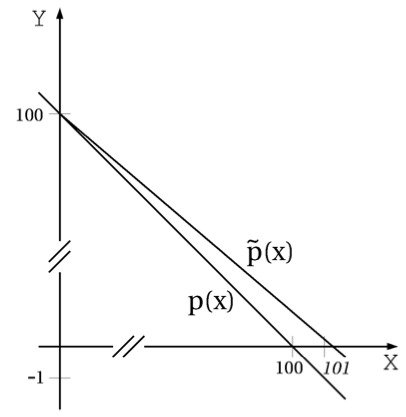
\includegraphics[width=0.39\linewidth]{error_amplification}
    \end{center}

    La causa di questa amplificazione dell'errore è evidente nel grafico sopra 
    riportato. In pratica il coefficiente $a_1$ rappresenta l'inclinazione
    della retta la quale, anche se alterata minimamente, comporta grossi
    errori per punti lontani dall'origine. 
    
    Lo stesso comportamento si ottiene perturbando anche solo $a_0$, entrambi
    i coefficienti o valutando in altri punti dell'intervallo.

    \vskip 0.1in 
    Procediamo, per questo esempio, all'analisi dell'errore inerente mediante
    la stima \ref{eq:numero_condizione_1}:
    \begin{equation*}
       \begin{aligned}
            E_{in} &= \left\lvert \frac{f(\tilde{a}_0, \tilde{a}_1,
            \tilde{x})-f(a_0,a_1,x)}{f(a_0,a_1,x)}\right\rvert \leq
            \left\lvert c_0\epsilon_0\right\rvert + 
            \left\lvert c_1\epsilon_1\right\rvert + 
            \left\lvert c_x\epsilon_x\right\rvert\\ 
            &= \left\lvert \frac{a_0}{p(x)}\epsilon_0\right\rvert +
            \left\lvert \frac{a_1x}{p(x)}\epsilon_1\right\rvert +
            \left\lvert \frac{x\alpha_1}{p(x)}\epsilon_x\right\rvert
       \end{aligned} 
    \end{equation*}
    e nel caso $a_0=100$, $a_1=-1$ e $x\in[100,101]$ con, per esempio, $x=101$
    si ha:
    $$=\left\lvert \frac{100}{-1}\epsilon_0\right\rvert + \left\lvert
    \frac{-101}{-1}\epsilon_1\right\rvert +
    \left\lvert \frac{-101}{-1}\epsilon_x\right\rvert$$
    da qui si vede come il problema è mal condizionato. Infatti una minima 
    perturbazione su uno dei coefficienti, per esempio, 
    $a_1$ dell'1\% ($\epsilon_0=0,\epsilon_1=1/100,\epsilon_x=0$),
    fa sì che l'errore relativo assuma il valore $101 \frac{1}{100}$ e cioè
    101 volte maggiore di quello sul dato iniziale.

    Dall'analisi fatta si evince che, per qualunque punto $x\in[100,101]$,
    questo comportamento sarà inevitabile in quanto una lieve modifica dei
    coefficienti ($\epsilon_0$ o $\epsilon_1\neq 0$) viene grandemente
    amplificata (coefficienti $c_0\text{ e }c_1$).
\end{example}
Generalizzando l'analisi fatta in questo esempio alla valutazione di un
generico polinomio $p(x)$ nella base canonica l'errore inerente si può
rappresentare come la somma di due componenti:
\begin{equation*}
    \begin{aligned}
        E_{in} &\leq 
        {\color{blue}\left\lvert \frac{a_0}{p(x)}\epsilon_0\right\rvert} + 
        {\color{blue}\left\lvert \frac{a_1x}{p(x)}\epsilon_1\right\rvert} + 
        {\color{blue}\left\lvert \frac{a_2x^2}{p(x)}\epsilon_2\right\rvert} + \ldots + 
        {\color{blue}\left\lvert \frac{a_nx^n}{p(x)}\epsilon_n\right\rvert} + 
        {\color{red}\left\lvert \frac{xp'(x)}{p(x)}\epsilon_x \right\rvert}\\
        &={\color{blue}E_{in1}}+{\color{red}E_{in2}}
    \end{aligned}
\end{equation*}
Si può desumere che:
\begin{itemize}
    \item $E_{in1}$ dipende da $p(x)$ e dai valori $a_ix^i$. Questi termini dipendono
   dalla base di rappresentazione;
   \item $E_{in2}$ dipende dal valore di $x$, dal polinomio in esame $p(x)$ e
       dalla sua derivata, per cui è un errore che non dipende dalla
       base di rappresentazione.
\end{itemize}
Pertanto, l'espressione di un polinomio può incidere sull'errore inerente
associato alla sua valutazione. Nel seguito vogliamo esaminare se è possibile
cambiare la base di rappresentazione al fine di ridurre l'errore inerente.

Consideriamo una base di $\mathbb{P}_n$ costituita da $n+1$ polinomi
linearmente indipendenti come \\$\{\phi_0(x),\phi_1(x),\ldots,\phi_n(x)\}$; allora
un generico polinomio $p(x)$ di grado al massimo $n$ 
può essere espresso come una combinazione lineare di questi polinomi:
$$p(x)=\displaystyle\sum_{i=0}^{n}b_i\phi_i$$
Se ripetiamo l'analisi fatta per determinare $E_{in}$ nel caso che $p(x)$ sia
rappresentato nella base $\{\phi_i\}$, avremo: 
$$E_{in}\leq \displaystyle\sum_{i=0}^{n}\left\lvert
c_i\epsilon_i\right\rvert+\left\lvert c_x\epsilon_x\right\rvert$$
con 
\begin{equation*}
   \begin{aligned}
       & {\color{blue}C_i=\frac{b_i\phi_i(x)}{p(x)}} &
       {\color{red}C_x=\frac{xp'(x)}{p(x)}}
   \end{aligned} 
\end{equation*}
L'idea è che, identificando una base di rappresentazione con valori
``piccoli'', potremmo ottenere un miglioramento sull'errore inerente $E_{in1}$.
\begin{example}
    Un primo esempio è rappresentato dalla base con centro
    $\{1,(x-c),(x-c)^2,\ldots,(x-c)^n\}$ con $c\in[a,b]$.
\end{example}
\subsection{Polinomi nella base di Bernstein}
Si potrebbe chiedersi se esista una base che, indipendentemente dal polinomio
considerato, il problema sia sempre ben condizionato. La risposta, in
generale, è no: spesso la scelta della base ottimale dipende dallo
specifico problema. Tuttavia, esiste una base, la base di Bernstein, che si
distingue come particolarmente efficace e versatile rispetto ad altre.
\begin{definition}
    Con funzione polinomiale in forma di Bernstein si intende un espressione del
    tipo 
    \begin{equation*}
        \begin{aligned}
       & p(x)=\displaystyle\sum_{i=0}^{n}b_iB_{i,n}(x) & \text{con }x\in[a,b]
        \end{aligned} 
    \end{equation*}
    dove i $B_{i,n}(x)$ sono i polinomi base di Bernstein definiti sull'intervallo
    $[a,b]$ da 
    \begin{equation} \label{eq:bernstein}
        \begin{aligned}
            B_{i,n}(x)=\binom{n}{i}\frac{(b-x)^{n-i}(x-a)^i}{(b-a)^n}
        \end{aligned} 
    \end{equation}
    e $b_0,b_1,\ldots,b_n\in \mathbb{R}$ sono i coefficienti nella base di
    Bernstein.
\end{definition}
con $\binom{n}{i}=\frac{n!}{i!(n-i)!}$.
\begin{itemize}
    \item \textbf{n=1} 
        \begin{equation*}
           \begin{aligned}
               B_{0,1}(x)&=\binom{1}{0}\frac{(b-x)^1(x-a)^0}{b-a}=\frac{b-x}{b-a}
                \\ 
               B_{1,1}(x)&=\binom{1}{0}\frac{(b-x)^0(x-a)^1}{b-a}=\frac{x-a}{b-a} 
           \end{aligned} 
        \end{equation*}
        \begin{center}
             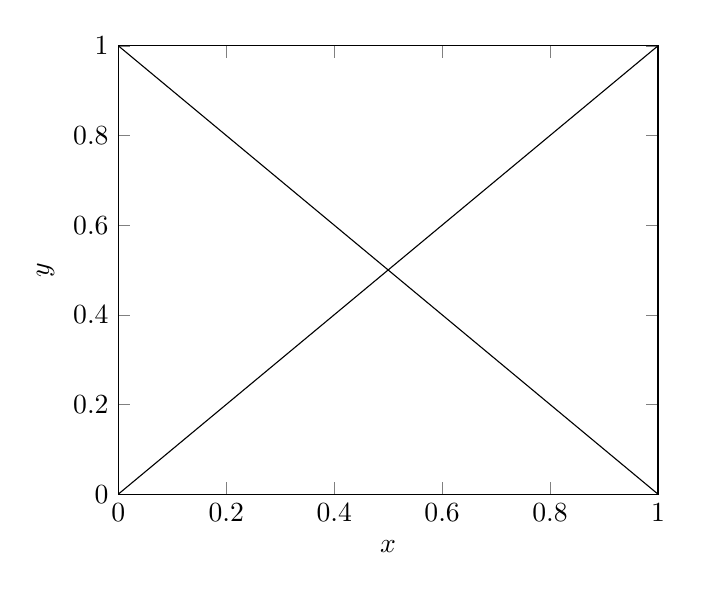
\begin{tikzpicture}
                \begin{axis}[
                    xlabel={$x$},
                    ylabel={$y$},
                    xmin=0, xmax=1,
                    ymin=0, ymax=1,
                ]
                \addplot[domain=0:1] {1-x};
                \addplot[domain=0:1] {x};
                \end{axis}
            \end{tikzpicture} 
        \end{center}
    \item \textbf{n=2}
        \begin{equation*}
           \begin{aligned}
               B_{0,2}(x)&=\binom{2}{0}\frac{(b-x)^2(x-a)^0}{(b-a)^2}=\frac{(b-x)^2}{(b-a)^2}
               \\ 
               B_{1,2}(x)&=\binom{2}{1}\frac{(b-x)^1(x-a)^1}{(b-a)^2}=\frac{(b-x)(x-a)}{(b-a)^2}
               \\
               B_{2,2}(x)&=\binom{2}{2}\frac{(b-x)^0(x-a)^2}{(b-a)^2}=\frac{(x-a)^2}{(b-a)^2}
           \end{aligned} 
        \end{equation*}
        \begin{center}
             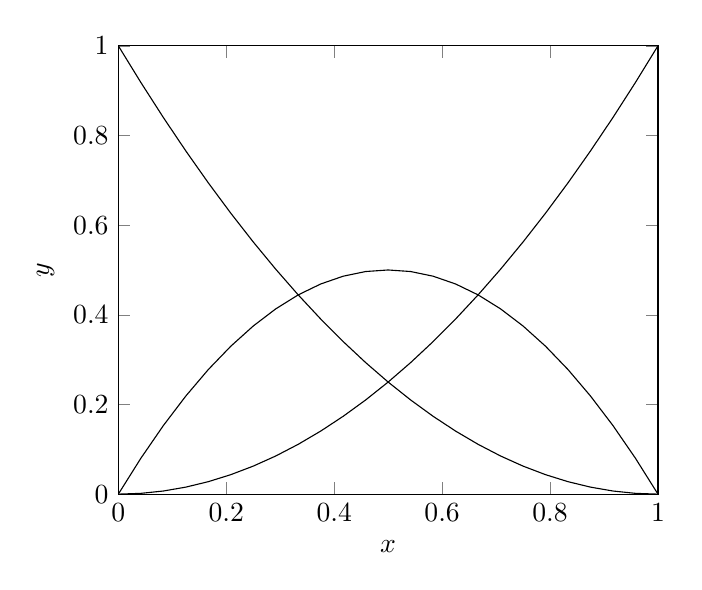
\begin{tikzpicture}
                \begin{axis}[
                    xlabel={$x$},
                    ylabel={$y$},
                    xmin=0, xmax=1,
                    ymin=0, ymax=1,
                ]
                \addplot[domain=0:1] {(1-x)^2};
                \addplot[domain=0:1] {2*x*(1-x)};
                \addplot[domain=0:1] {x^2};
                \end{axis}
            \end{tikzpicture} 
        \end{center}
\end{itemize}
\begin{example}
   Riprendiamo il polinomio $p(x)=100-x$ e lo riscriviamo nella base di
   Bernstein:
   \begin{equation*}
       \begin{aligned}
           & B_{0,1}(x)=\binom{1}{0}\frac{(101-x)1}{1}=101-x &
           B_{1,0}(x)=\binom{1}{1}\frac{1(x-100)}{1}=x-100
       \end{aligned}
   \end{equation*}
   da cui 
   \begin{equation*}
       \begin{aligned}
           p(x)&=100-x=b_0B_{0,1}(x)+b_1B_{1,1}(x)\\
               &=b_0(101-x)+b_1(x-100)
       \end{aligned}
   \end{equation*}
   Ossia $b_0=0$ e $b_1=-1$.
   
   Rieseguendo l'analisi sull'errore inerente si ha:
   \begin{equation*}
       \begin{aligned}
           E_{in}&\leq \left\lvert c_0\epsilon_0 \right\rvert 
            + \left\lvert c_1\epsilon_1\right\rvert 
            + \left\lvert c_x\epsilon_x\right\rvert\\
                 &= \left\lvert \frac{b_0(101-x)}{p(x)}\epsilon_0\right\rvert
                 + \left\lvert \frac{b_1(x-100)}{p(x)}\epsilon_1\right\rvert
             + \left\lvert \frac{xp'(x)}{p(x)}\epsilon_x\right\rvert \\
             \alignedintertext{valutandoli in $x=101$ si ha:}
                 &=\left\lvert \frac{0(101-101)}{-1}\epsilon_0\right\rvert + 
                 \left\lvert \frac{-1(1)}{-1}\epsilon_1\right\rvert +
                 \left\lvert \frac{101(-1)}{-1}\epsilon_x\right\rvert \\ 
                 &= \left\lvert \epsilon_1 \right\rvert + \left\lvert
                 101\epsilon_x\right\rvert
       \end{aligned}
   \end{equation*}
   Siamo riusciti a rendere ``piccoli'' i numeri di condizioni che dipendono
   dalla base di rappresentazione. Tuttavia, il termine $c_x$, essendo
   indipendente dalla base di rappresentazione scelta, potrebbe causare un
   incremento significativo dell'errore inerente.
\end{example}
Considerando il problema evidenziato nell'esempio, si può fare qualcosa?

\subsubsection{Cambio di variabile}
I polinomi godono della proprietà di essere \textbf{invarianti per traslazione e scala
dell'intervallo di definizione o cambio di variabile}. Questo significa che,
per qualsiasi dato polinomio $p(x)$, definito in un intervallo $[a,b]$, è
sempre possibile individuare un altro polinomio che assume gli stessi valori
all'interno di un intervallo che è stato traslato o scalato. Questo permette
di definire un'applicazione (mapping) tra i due intervalli $[a,b]$ e, per
esempio, $[0,1]$
\begin{equation} \label{eq:cambio_variabile}
   \begin{aligned}
       & x\in[a,b]\rightarrow t\in[0,1] \\ 
       & t=\frac{x-a}{b-a} \text{ o viceversa }x=a+t(b-a)
   \end{aligned} 
\end{equation}
\begin{center}
    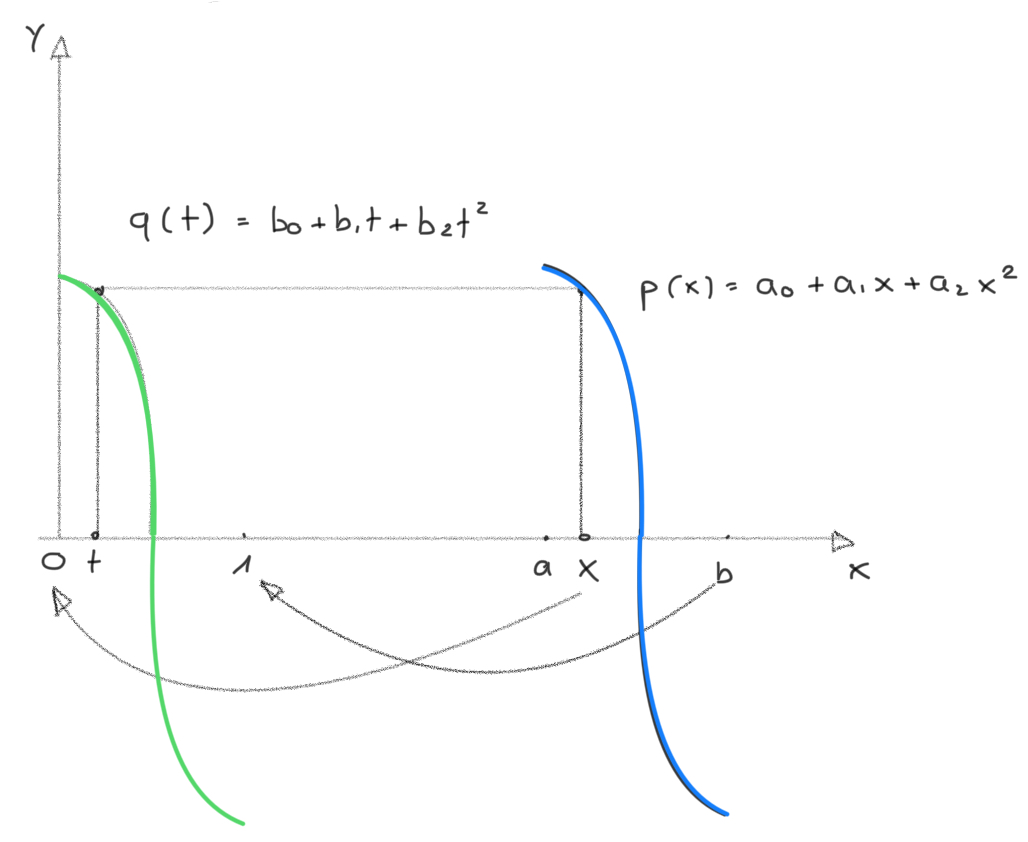
\includegraphics[width=0.5\linewidth]{cambio_variabile}
\end{center}
Per effettuare un cambio di variabile, possiamo sostituire, all'interno del
polinomio, $x$ con $a+t(b-a)$. Otteniamo un nuovo polinomio espresso in
termini di $t$ piuttosto che di $x$. 

Consideriamo un polinomio $p(x)$ espresso nella base di Bernstein:
$$p(x)=\displaystyle\sum_{i=0}^{n}b_iB_{i,n}(x)\quad \text{con }x\in[a,b]$$
Vogliamo effettuare un cambio di variabile da $x$ a $t$, con $t\in[0,1]$.
Riscriviamo la \ref{eq:bernstein} nel seguente modo:
$$=\binom{n}{i}\left(\frac{b-x}{b-a}\right)^{n-i}\left(\frac{x-a}{b-a}\right)^i$$
Sostituendo $x$ con $a+t(b-a)$, otteniamo:
\begin{equation*}
   \begin{aligned}
       &=\binom{n}{i}\left(\frac{\cancel{(b-a)}(1-t)}{\cancel{b-a}}\right)^{n-i}\left(
       \frac{\cancel{a}+t\cancel{(b-a)}-\cancel{a}}{\cancel{b-a}}\right)^i\\ 
       &=\binom{n}{i}(1-t)^{n-i}t^i=B_{i,n}(t)
   \end{aligned} 
\end{equation*}
Il cambio di variabile ha trasformato la base di Bernstein in funzione di $t$,
mantenendo inalterati i coefficienti $b_i$. Pertanto, il polinomio dopo il
cambio di variabile è:
$$p(t)=\displaystyle\sum_{i=0}^{n}b_iB_{i,n}(t)\quad \text{con }t\in[0,1]$$
Quindi un cambio di variabile, per un polinomio nella base di Bernstein, non
comporta alcun errore o costo computazionale sui coefficienti in quanto
restano uguali.

Ma come ci aiuta esattamente il cambio di variabile a ridurre il numero di
condizione $c_x$?

Consideriamo la trasformazione:
$$\frac{xp'(x)}{p(x)}\rightarrow \frac{tp'(t)}{p(t)}$$
Se effettuiamo un cambio di variabile da $x$ a $t$, dove $t$ è definito
nell'intervallo $[0,1]$, stiamo effettivamente ridimensionando la variabile $x$.
Questa operazione ha un impatto anche sulla sua derivata. Infatti, il
ridimensionamento di questo intervallo, per effetto della scala, 
potrebbe attenuare o "rilassare" la derivata del polinomio.

\begin{example}
   Riprendiamo il polinomio $p(x)=100-x$. Questo può essere espresso nella
   base di Bernstein come
   $p(x)=-1\underbrace{(x-100)}_{B_{1,1}(x)}$ con $x\in[100,101]$. Ora, 
   effettuiamo il cambio di variabile in $t\in[0,1]$.

   I polinomi di Bernstein in termini di $t$ sono:
   \begin{equation*}
       \begin{aligned}
           & B_{0,1}(t)=1-t & B_{1,1}(t)=t
       \end{aligned}
   \end{equation*}
   In termini di $t$, il polinomio $p(x)$ diventa:
   $$q(t)=-1\underbrace{(t)}_{B_{1,1}(t)}$$
   Se valutiamo in $x=101$, questo corrisponde a $t=1$. Calcoliamo ora, $c_t$:
   $$c_t=\frac{tq'(t)}{q(t)}=\frac{1}{-1}(-1)=1$$
    Grazie al cambio di variabile, $c_t$ è stato ridotto a un valore che non
    amplifica l'errore.
\end{example}
\subsubsection{Proprietà dei polinomi di Bernstein}
Da ora in poi useremo sempre i polinomi di Bernstein nell'intervallo $[0,1]$.
\begin{definition}
    Il polinomio di Bernstein definito sull'intervallo $[0,1]$ è dato da:
    $$B_{in}=\binom{n}{i}(1-x)^{n-i}\cdot x^{i}\quad \text{ con }x\in[0,1]$$
\end{definition}
Inoltre, i polinomi della base di Bernstein $B_{i,n}(x)$ godono delle seguenti
proprietà:
\begin{enumerate}
    \item $B_{i,n}\geq0\quad i=0,\ldots,n\quad \forall x\in[0,1]$;
        \begin{itemize}
            \item Il valore del polinomio è sempre \underline{non negativo};
            \item $B_{i,n}=0$ agli estremi dell'intervallo.
                \begin{equation*}
                   \begin{aligned}
                       & B_{0,n}(x)=(1-x)^n &\text{tutti gli zero in 1 e
                       nessuno zero in 0}\\
                       & B_{1,n}(x)=\binom{n}{1}(1-x)^{n-1}x^1 & \text{uno
                       zero in 0 ed $n$ zeri in 1}\\
                       & \vdots \\
                       & B_{n,n}(x)=x^n & \text{tutti gli zero in 0 e
                       nessuno zero in 1}
                   \end{aligned} 
                \end{equation*}
                \begin{center}
                    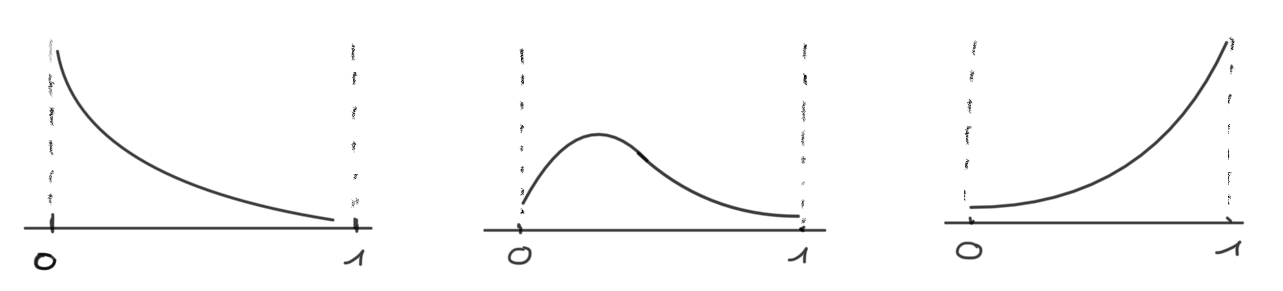
\includegraphics[width=0.8\linewidth]{bernstein_zeros}
                \end{center}
        \end{itemize}
    \item \textbf{Partizione dell'unità}:
        per ogni $x$ nell'intervallo $[0,1]$, la somma dei valori dei
        polinomi di Bernstein è sempre uguale a 1.
        $$\displaystyle\sum_{i=0}^{n}B_{in}(x)=1\quad \forall x\in[0,1]$$
        \begin{center}
            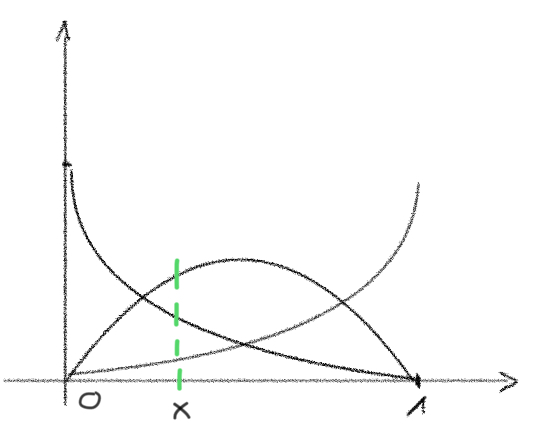
\includegraphics[width=0.3\linewidth]{bernstein_one_sum}
        \end{center}
    \item Per le proprietà precedenti, $p(x)$ espresso nella base di Bernstein
        è una combinazione convessa dei $b_i$, da cui segue
        $$\underset{i}{\min\{b_i\}}\leq p(x)\leq \underset{i}{\max\{b_i\}}$$
        \begin{center}
            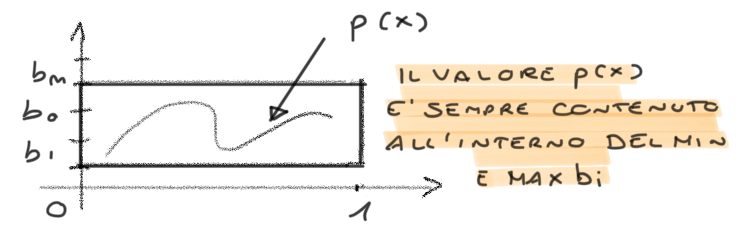
\includegraphics[width=0.4\linewidth]{bernstein_convex}
        \end{center}
        Ciò suggerisce che affinché il polinomio $p(x)$ possa avere zeri
        reali, i coefficienti $b_i$ devono essere sia positivi che negativi.
    \item Valutando il polinomio in $x=0$, solo $B_{0,n}(0)$ ha valore 1,
        mentre tutti gli altri polinomi di Bernstein sono nulli. Di
        conseguenza, $p(0)$ corrisponde al coefficiente $b_0$. Analogamente,
        in $x=1$, $p(1)$ coincide con $b_n$ dato che solo $B_{n,n}(1)$ è non
        nullo e vale 1.
        \begin{equation*}
            \begin{aligned}
               & p(0)=b_0 & p(1)=b_n 
            \end{aligned}
        \end{equation*}
\end{enumerate}
Ma se volessimo valutare un polinomio nella base di Bernstein in un punto interno, 
anziché agli estremi? Poiché gli algoritmi di valutazione polinomiale che
abbiamo visto finora sono pensati per la base canonica, è necessario
introdurre due nuovi algoritmi specificamente pensati per la base di
Bernstein.
\subsubsection{Valutazione di un polinomio nella base di Bernstein}
\paragraph{Formula ricorrente base di Bernstein.}
I polinomi base di Bernstein di grado $n$, sono determinabili dai polinomi di
Bernstein di grado $n-1$, dalla seguente formula ricorrente
$$B_{i,n}(x)=xB_{i-1,n-1}(x)+(1-x)B_{i,n-1}(x)$$
con $B_{0,0}(x)=1$ e $B_{i,n}(x)=0$ per ogni $i\notin\{0,n\}$.
\begin{itemize}
    \item[\textbf{Passi}:]
    \begin{enumerate}
        \item \textbf{Inizializzazione}: si crea un vettore $B$ di lunghezza $n+1$, 
            inizializzato con tutti zeri tranne il primo elemento ($B_{0,0}$) che
            sarà 1. Questo vettore conterrà i valori dei polinomi base di
            Bernstein.
        \item \textbf{Valutazione delle funzioni base di Bernstein}: si calcolano
            iterativamente i valori dei polinomi base di Bernstein di grado $n$
            usando la formula ricorrente.
            \begin{center}
                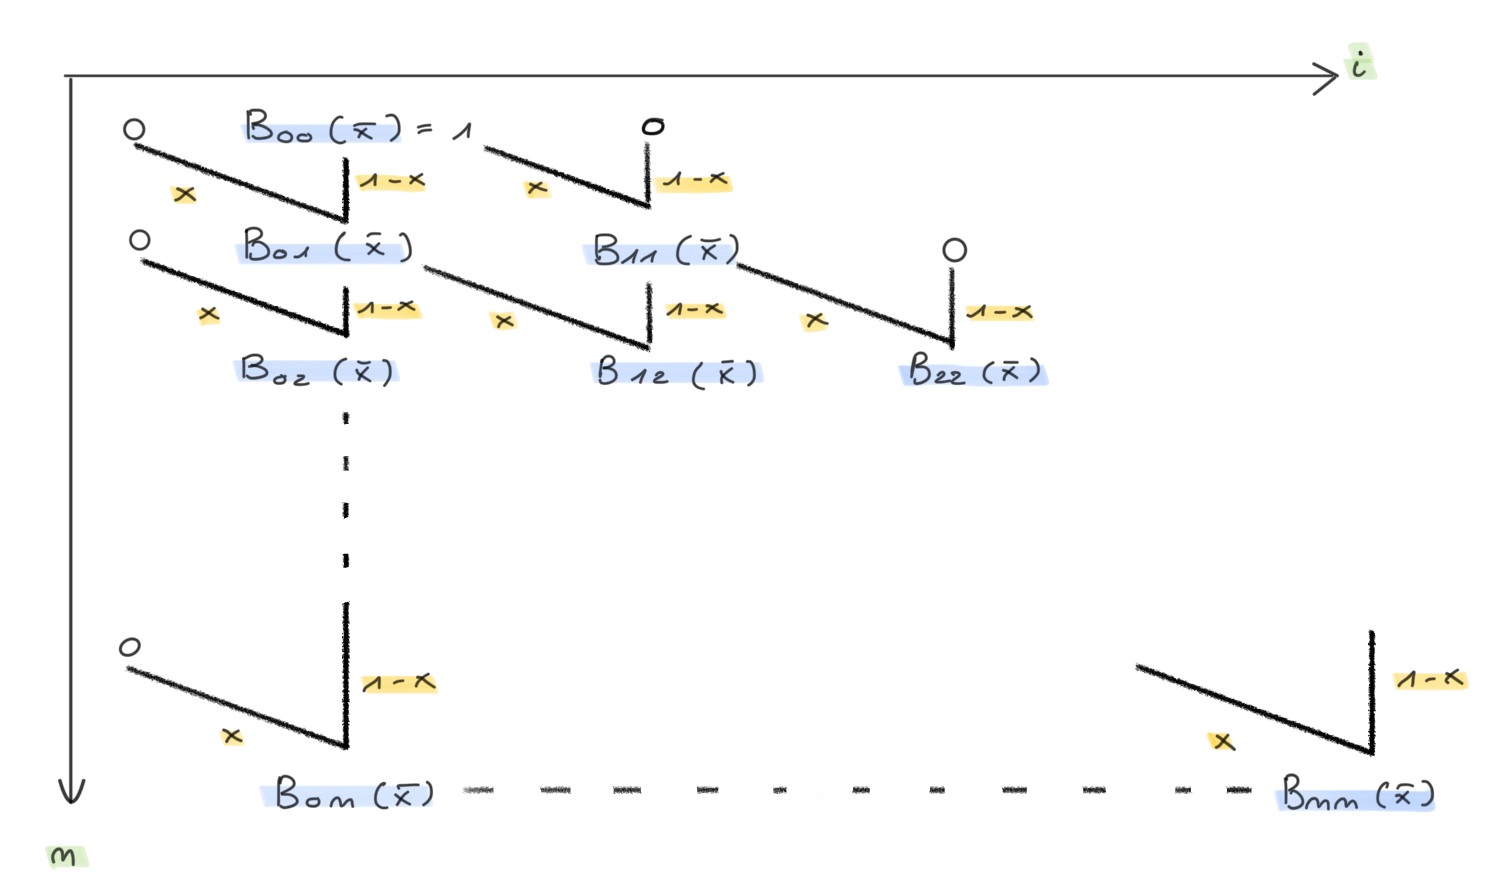
\includegraphics[width=0.8\linewidth]{bernstein_ricorsive}
            \end{center}
        \item \textbf{Calcolo di
            $p(x)=\displaystyle\sum_{i=0}^{n}b_iB_{in}(\bar{x})$}: si esegue il prodotto
            scalare del vettore riga $b$ e
            il vettore colonna $B^T$ per ottenere il valore del polinomio in
            $\bar{x}$.
    \end{enumerate}
\end{itemize}
\begin{lstlisting}[language=Python]
def bernstein_evaluation(b, x_bar):
    n = len(b)
    B = np.zeros((n,n))
    B[0][0] = 1.

    for i in range(1,n):
        for j in range(0,i+1):
            if j == 0:
                B[i][j] = (1-x_bar) * B[i-1][j]
            elif j == i:
                B[i][j] = x_bar * B[i-1][j-1]
            else:
                B[i][j] = x_bar * B[i-1][j-1] + (1-x_bar)*B[i-1][j]
    return sum([b[i] * B[n-1][i] for i in range(n)])
\end{lstlisting}
Quando si utilizza l'algoritmo per valutare un polinomio nella base di
Bernstein:
\begin{itemize}
    \item Il calcolo del valore dei polinomi base $B_{i,n}(\bar{x})$ per
        $i=0,\ldots,n$ necessita di $\frac{n(n+1)}{2}$ addizioni e
        $n(n+1)$ moltiplicazioni.
    \item Per ottenere il valore finale del polinomio in $\bar{x}$ attraverso
        la combinazione lineare dei polinomi base e dei coefficienti del
        polinomio, sono necessarie ulteriori $n$ addizioni e $n$
        moltiplicazioni
\end{itemize}
In totale, l'algoritmo ha un costo computazionale di $\mathcal{O}(n^2)$. 
Anche se questo costo potrebbe sembrare alto, va sottolineato che l'algoritmo
è numericamente stabile, specialmente, nel calcolo dei polinomi base.
\paragraph{Algoritmo di de Casteljau.} Un'alternativa all'algoritmo proposto è
l'algoritmo di de Casteljau, che deriva dall'applicare ripetutamente la
formula ricorrente all'espressione del polinomio. Vediamolo: 
\begin{equation*}
  \begin{aligned}
      p(x)&=\displaystyle\sum_{i=0}^{n}b_iB_{i,n}(x)\overset{\text{def}}{=}\displaystyle\sum_{i=0}^{n}b_i(xB_{i-1,n-1}(x)+(1-x)B_{i,n-1}(x))\\
          &=\displaystyle\sum_{i=0}^{n}b_ixB_{i-1,n-1}(x)+\displaystyle\sum_{i=0}^{n}b_i(1-x)B_{i,n-1}(x)
          \\ 
          \alignedintertext{A questo punto, dobbiamo notare che il termine $B_{-1,n-1}$ non
          esiste. Inoltre, dato che la sommatoria effettivamente va solo fino
      a $n-1$, il termine $B_{n,n-1}=0$. Dunque, regolando gli indici,
  abbiamo:}
          &=\displaystyle\sum_{i=0}^{n-1}b_{i+1}xB_{i,n+1}(x)+\displaystyle\sum_{i=0}^{n-1}b_i(1-x)B_{i,n-1}(x)\\
          \alignedintertext{Raccogliendo:}
          &=
          \displaystyle\sum_{i=0}^{n-1}{\color{blue}\left[b_{i+1}x+b_i(1-x)\right]}B_{i,n-1}(x)\\ 
          &=\displaystyle\sum_{i=0}^{n-1}{\color{blue}b_i^{[1]}}B_{i,n-1}(x) \\
          \alignedintertext{Riapplicando la formula ricorrente più volte, alla
          fine si ottiene:}
          &=\displaystyle\sum_{i=0}^{0}b_0^{[n]}\overbrace{B_{0,0}(x)}^1=b_0^{[n]}
  \end{aligned}  
\end{equation*}
Si ha quindi il seguente algoritmo:
\begin{equation} \label{eq:de_casteljau}
   \begin{aligned}
       b_{i}^{[j]}=xb_{i+1}^{[j-1]}+(1-x)b_{i}^{[j-1]}
   \end{aligned} 
\end{equation}
con $j=0,\ldots,n$ e $i=0,\ldots,n-j$.

Si inizia con i coefficienti iniziali del polinomio e si applica
iterativamente l'equazione \ref{eq:de_casteljau} fino a quando non si ottiene
$b_{0}^{[n]}$. Quest'ultimo valore corrisponde al valore del polinomio quando
viene valutato in $x$.
\begin{center}
    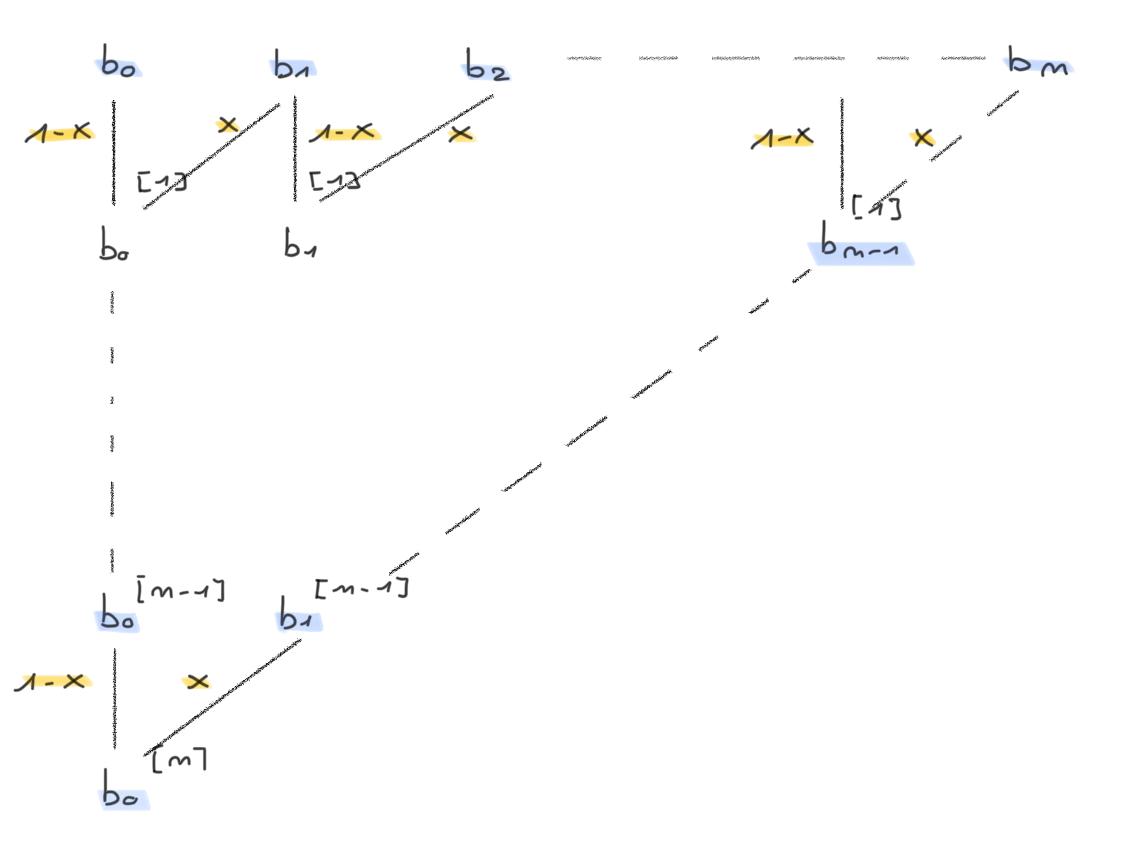
\includegraphics[width=0.58\linewidth]{bernstein_decasteljau}
\end{center}
\begin{lstlisting}[language=Python]
def de_casteljau(b, x_bar):
    if len(b) == 1:
        return b[0]
    
    b_new = []
    for i in range(len(b)-1):
        b_new.append(x_bar * b[i+1] + (1-x_bar) * b[i])
    
    return de_casteljau(b_new, x_bar)
\end{lstlisting}
Quando si utilizza l'algoritmo di Casteljau per valutare un polinomio nella
base di Bernstein:
\begin{itemize}
    \item Il calcolo del coefficiente $b_{0}^{[n]}$ necessita di $\frac{n(n+1)}{2}$
    addizioni e $n(n+1)$
\end{itemize}
Il costo totale dell'algoritmo è di $\mathcal{O}(n^2)$. Tuttavia, è meno
costoso rispetto al precedente algoritmo. Ciò è dovuto al fatto che
l'algoritmo di Casteljau elimina la necessità di calcolare esplicitamente la
combinazione lineare per determinare il valore di $p(x)$.
\begin{example}
    Si consideri il polinomio nella base di Bernstein:
    $$p(x)=2\overbrace{B_{0,3}}^{b_0}(x)+2\overbrace{B_{2,3}}^{b_2}(x)+0\overbrace{B_a{1,3}(x)}^{b_1}+0\overbrace{B_{3,3}(x)}^{b_3}$$
    Applicare l'algoritmo di de Casteljau ai seguenti punti: 
    $$x=\left[0, \frac{1}{3},\frac{1}{2}, \frac{2}{3}, 1\right]$$
    Infine, disegnare un grafico per i punti $p(x)$.
    
    Eseguendo l'algoritmo, otteniamo:
    \begin{itemize}
       \item$p(0)=2, p(1)=0$ dati dalle proprietà dei polinomi di Bernstein;
       \item $p(\frac{1}{2})=1, p(\frac{1}{3})=\frac{28}{27},
       p(\frac{2}{3})=\frac{26}{27}$.

       \begin{center}
           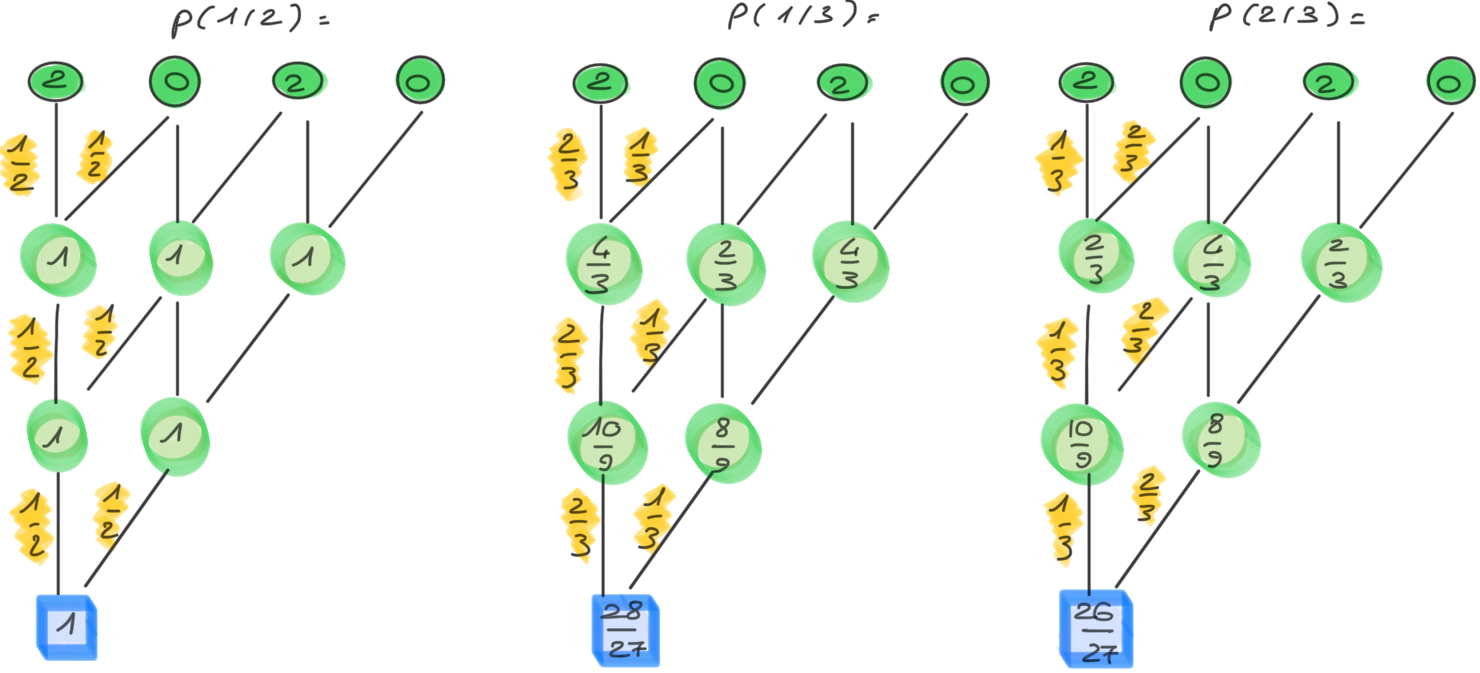
\includegraphics[width=0.9\linewidth]{de_casteljau2}
       \end{center}
    \end{itemize}

    \begin{center}
        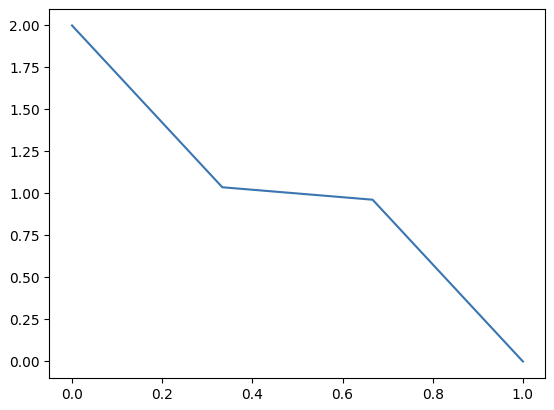
\includegraphics[width=0.5\linewidth]{de_casteljau}
    \end{center}
\end{example}
I polinomi base di Bernstein rappresentano una delle basi preferite per la
rappresentazione di curve, in particolare per le curve di Bézier.
Una curva 2D è definita come segue:
\[
C(t) = \left( f(t), g(t) \right), \quad \text{dove} \quad t \in [0,1].
\]
dove \( t \in [0,1] \). Ogni \( t \) individua un punto sulla curva.

Utilizzando i polinomi di Bernstein come base, possiamo esprimere le funzioni
\( f(t) \) e \( g(t) \) come segue:
\begin{equation*}
    \begin{aligned}
        &f(t)=\displaystyle\sum_{i=0}^{n}x_iB_{in}(t)
        &g(t)=\displaystyle\sum_{i=0}^{n} y_iB_{in}(t) 
    \end{aligned} 
\end{equation*}

In termini vettoriali, la curva può essere descritta come una funzione
vettoriale nella base di Bernstein:

$$C(t) = \sum_{i=0}^{n} P_i B_{in}(t)$$

dove \(P_i = (x_i, y_i)\) rappresentano i punti di controllo.

Le curve di Bézier sono utilizzate nel disegno su calcolatore e nei font
vettoriali. In questi font, un carattere è definito da curve. A differenza
delle immagini raster, i disegni vettoriali mantengono nitidezza a qualsiasi
livello di ingrandimento. Così, zoomando su un carattere o un disegno
vettoriale, non si perde qualità.
\newpage
\section{Interpolazione polinomiale}
\paragraph{Interpolazione di dati.} Il problema dell'interpolazione di dati
consiste nel trovare un polinomio che passi per un insieme di punti $(x_i,
y_i)$ dati. Più formalmente, si cerca un polinomio $p(x)$ appartenente
all'insieme dei polinomi $\mathbb{P}_n$ tale che $p(x_i)=y_i$ per ogni
$i=0,\ldots,n$.

In questo problema, abbiamo a disposizione gli $y_i$ - i valori che
desideriamo che il nostro polinomio assuma -  e gli $x_i$ - i punti
corrispondenti a questi valori. Ciò che manca sono i coefficienti del
polinomio, indicati con $a$.

Potremmo considerare l'interpolazione come il problema inverso ella
valutazione di un polinomio. Nella valutazione, abbiamo i coefficienti del
polinomio e gli $x_i$ dove desideriamo valutare il polinomio. Invece,
nell'in-terpolazione, abbiamo i valori $y_i$ del polinomio e gli $x_i$, ma non
conosciamo i coefficienti.

In pratica, i dati potrebbero provenire, ad esempio, da misurazioni
sperimentali di un fenomeno e vogliamo rappresentarli con una funzione. Una
volta identificato un polinomio interpolante adatto, questo può essere
utilizzato per prevedere il comportamento della funzione all'interno
dell'intervallo di interesse, incluso in punti che non sono stati
originariamente misurati.
\begin{center}
    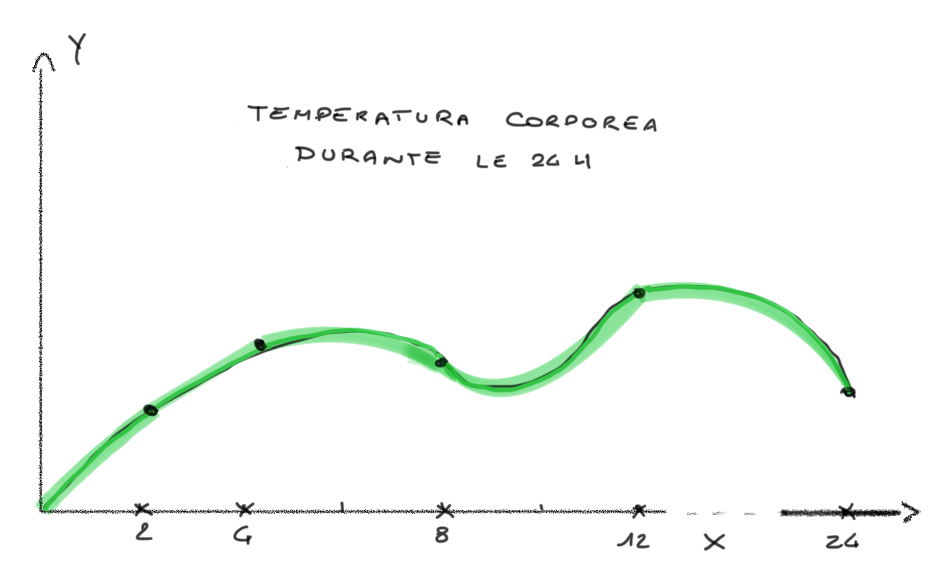
\includegraphics[width=0.5\linewidth]{temperature}
\end{center}
\paragraph{Interpolazione di funzioni.}
Il problema dell'interpolazione di funzioni mira a trovare un polinomio che
approssima una data funzione $f(x)$ in un intervallo $x\in[a,b]$. Questo
comporta:
\begin{enumerate}
    \item \textbf{Selezione dei punti dell'interpolazione}:
        \begin{itemize}
            \item A differenza dell'interpolazione di dati dove gli $x_i$ sono
                dati, qui scegliamo autonomamente i punti $x_i$ nell'intervallo
                $[a,b]$, con $i=0,\ldots,n$.
            \item La scelta di questi punti è fondamentale: una selezione
                appropriata può portare a una rappresentazione accurata della
                funzione originale, mentre una scelta inadeguata può portare
                un'appros-simazione imprecisa.
        \end{itemize}
    \item \textbf{Costruzione del polinomio}:
        \begin{itemize}
            \item Si determina un polinomio $p(x)\in \mathbb{P}_n$ tale che
                $p(x_i)$ coincida con $f(x_i)$ per ogni $i=0,\ldots,n$.
        \end{itemize}
    \item \textbf{Valutazione dell'errore}:
        \begin{itemize}
            \item Una volta costruito il polinomio, si valuta l'errore
                $\left\lvert f(x) - p(x)\right\rvert$ per ogni $x\in[a,b]$ per
                misurare l'accuratezza dell'approssimazione.
        \end{itemize}
\end{enumerate}
\subsection{Esistenza e unicità dell'interpolazione polinomiale}
\begin{theorem}
    Dati $n+1$ punti $(x_i,y_i)$, $i=0,\ldots,n$ con $x_i$ distinti, allora
    esiste ed è unico il polinomio $p\in \mathbb{P}_n$ che verifica le
    condizioni
    $$p(x_i)=y_i\quad i=0,\ldots,n$$
\end{theorem}
\begin{proof}\leavevmode\\
    Si consideri $p(x)$ in forma canonica 
    $$p(x)=a_0+a_1x+\ldots+a_nx^n$$
    Imponendo le $n+1$ condizioni di interpolazione, cioè che
    $p(x_i)=y_i$ con $i=0,\ldots,n$, otteniamo:
    $$\begin{cases}
        a_0+a_1x_0+a_2x_{0}^2\ldots+a_nx_0^n&=y_0\\ 
        a_0+a_1x_1+a_2x_{1}^2\ldots+a_nx_1^n&=y_1\\ 
        \ldots & \vdots \\
        a_0+a_1x_n+a_2x_{n}^2\ldots+a_nx_n^n&=y_n
    \end{cases}$$
    Cioè un sistema lineare di $n+1$ equazioni in $n+1$ incognite; se tale
    sistema ammette una ed una sola soluzione, allora tale sarà il polinomio.
    In forma matriciale il sistema si presenterà come:
    \begin{equation}
       \begin{aligned}
           Va=y
       \end{aligned}
    \end{equation}
    con 
    \begin{equation*}
       \begin{aligned}
           V&=\begin{bmatrix}
               1 & x_0 & x_{0}^2 & \ldots & x_{0}^n \\ 
               1 & x_1 & x_{1}^2 & \ldots & x_{1}^n \\ 
               \ldots \\
               1 & x_n & x_{n}^2 & \ldots & x_{n}^n \\ 
           \end{bmatrix} &
            a&=\begin{bmatrix}
               a_0 \\ 
               a_1 \\ 
               \vdots \\ 
               a_n
           \end{bmatrix} &
           y&=\begin{bmatrix}
               y_0 \\ 
               y_1 \\ 
               \vdots \\ 
               y_n
           \end{bmatrix}
       \end{aligned} 
    \end{equation*}
    il sistema $Va=y$ ammette una e una sola soluzione se e solo se la matrice
    $V$, conosciuta come matrice di Vandermonde, è non singolare, il che si
    verifica se e solo se il $\det(V)\neq 0$. Il determinante della matrice di
    Vandermonde può essere espresso come:
    $$\det(V)=\prod_{i,j=0,j>i}^{n}(x_j-x_i)$$ che nelle ipotesi che i punti
    $x_i$ siano distinti risulta sempre non nullo. Ciò dimostra che il sistema
    lineare ha un'unica soluzione e quindi $p(x)$ esiste ed è unico.
\end{proof}
La dimostrazione del Teorema fornisce anche un metodo per procedere alla
determinazione del polinomio interpolante risolvendo il sistema lineare.
\begin{example}
    Siano dati il set di punti $x=[0,1,2],y=[0,1,0]$. Si determini il polinomio
    che interpola i dati.

    In base al teorema visto, il polinomio che interpola questi dati esiste ed
    è unico, e può essere trovato in $\mathbb{P}_2$, ovvero
    $p(x)=a_0+a_1x+a_2x^2$.
    \begin{equation*}
       \begin{aligned}
           \begin{bmatrix}
               1 & 0 & 0 \\ 
               1 & 1 & 1 \\ 
               1 & 2 & 4
           \end{bmatrix}
           \begin{bmatrix}
               a_0 \\ 
               a_1 \\ 
               a_2 
           \end{bmatrix}= 
           \begin{bmatrix}
               0 \\ 
               1 \\ 
               0
           \end{bmatrix} \\
           =\begin{bmatrix}
               1 & 0 & 0 & | & 0\\ 
               1 & 1 & 1 & | & 1\\ 
               1 & 2 & 4 & | & 0
           \end{bmatrix}\\
           =\begin{bmatrix}
               1 & 0 & 0 & | & 0\\ 
               \frac{3}{4} & \frac{1}{2} & 0 & | & 1\\ 
               1 & 2 & 4 & | & 0
           \end{bmatrix}\\
           =\begin{bmatrix}
               1 & 0 & 0 & | & 0\\ 
               0 & \frac{1}{2} & 0 & | & 1\\ 
               0 & 2 & 4 & | & 0
           \end{bmatrix}\\
           =\begin{bmatrix}
               1 & 0 & 0 & | & 0\\ 
               0 & \frac{1}{2} & 0 & | & 2\\ 
               0 & 0 & 4 & | & -4
           \end{bmatrix}\\
           =\begin{bmatrix}
               1 & 0 & 0 & | & 0\\ 
               0 & 1 & 0 & | & 2\\ 
               0 & 0 & 1 & | & -1
           \end{bmatrix}\\
           p(x)=0+2x-x^2
       \end{aligned} 
    \end{equation*}
Si osserva inoltre che il polimonio trovato è il polinomio di grado
\textsc{minimo} che interpola i dati in $\mathbb{P}_n$.
    \begin{center}
        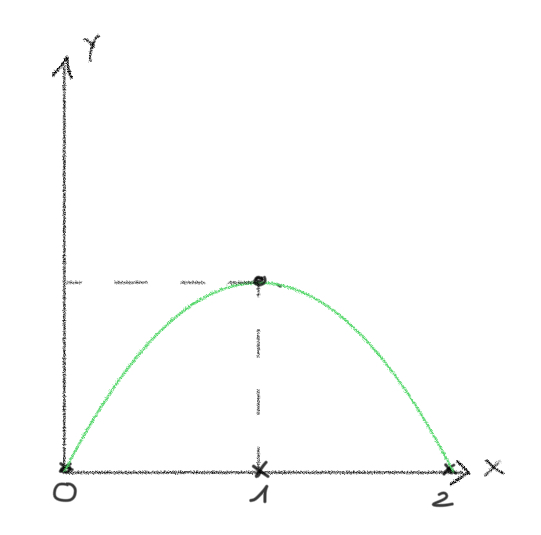
\includegraphics[width=0.25\linewidth]{interpolation_linear_system}
    \end{center}
\end{example}
\subsection{Metodi di costruzione}
Ora esamineremo vari metodi di interpolazione polinomiale, ciascuno basato su
una diversa base polinomiale, allo scopo di identificare quale tra queste 
sia la migliore.
\subsubsection{Base di Newton}
Siano dati $n+1$ punti distinti $(x_1,y_1)$ con $i=0,\ldots,n$. Il polinomio
interpolante nella forma di Newton è costruito su una particolare base chiamata base
di Newton, che viene costruita sui punti $x_i,\ i=0,\ldots,n$.

La base di Newton è costituita da $n+1$ funzioni base linearmente
indipendenti
$$1,(x-x_0),(x-x_0)(x-x_1),\ldots,(x-x_0)(x-x_1)\cdots(x-x_{n-1})$$
e forma una base polinomiale per lo spazio $\mathbb{P}_n$.

Il polinomio interpolante nella base di Newton può essere scritto come combinazione lineare di
queste funzioni base:
$$p(x)=b_0+b_1(x-x_0)+b_2(x-x_0)(x-x_1)+\ldots+b_n(x-x_0)(x-x_1)\cdots(x-x_n)$$

Imponendo le condizioni di interpolazione a questo polinomio si ottiene un
sistema di $n+1$ equazioni in $n+1$ incognite:
\begin{equation*}
    \begin{aligned}
        &p(x_0)=y_0\Rightarrow
              &b_0+b_1\overbrace{(x_0-x_0)}^0+b_2\overbrace{(x_0-x_0)}^0(x_0-x_1)+\ldots+b_n\overbrace{(x_0-x_0)}^0(x_0-x_1)\cdots(x_0-x_{n-1})=y_0\\ 
              & &b_0=y_0 \\                                                                                                                            
        &p(x_1)=y_0\Rightarrow
        &b_0+b_1(x_1-x_0)+b_2(x_1-x_0)\overbrace{(x_1-x_1)}^0+\ldots+b_n(x_1-x_0)\overbrace{(x_1-x_1)}^0\cdots(x_1-x_{n-1})=y_0\\ 
              & &b_0+b_1(x_1-x_0)=y_0 \\ 
        &\vdots & \vdots \\
        &p(x_n)=y_n\Rightarrow
              &b_0+b_1(x_n-x_0)+b_2(x_n-x_0)(x_n-x_1)+\ldots+b_n(x_n-x_0)(x_n-x_1)\cdots(x_n-x_{n-1})=y_n\\ 
    \end{aligned}
\end{equation*}
Questo sistema può essere espresso in forma matriciale come:
$$Nb=y$$
con
\begin{equation*}
   \begin{aligned}
       N&=\begin{bmatrix}
           1 & 0 & 0 & \ldots & 0 \\ 
           1 & (x_1-x_0) & 0 & \ldots & 0 \\ 
           \vdots & \vdots & \ddots & & \vdots \\ 
           1 & (x_n-x_0) & (x_n-x_0)(x_n-x_1) & \ldots & (x_n-x_0)\cdots(x_n-x_{n-1})
       \end{bmatrix} & 
        c&=\begin{bmatrix}
            b_0 \\ 
            b_1 \\ 
            \vdots \\ 
            b_n
       \end{bmatrix} & 
       y&=\begin{bmatrix}
           y_0 \\ 
           y_1 \\ 
           \vdots \\ 
           y_n
       \end{bmatrix}
   \end{aligned} 
\end{equation*}
Poiché la matrice $N$ è triangolare inferiore, il sistema è facilmente
risolvibile per sostituzione in avanti. Ciò fornisce i coefficienti $b_i$, che
rappresentano il polinomio che interpola i dati.
\begin{lstlisting}[language=Python]
def calculate_newton_base(x_bar, x):
    return np.prod([x_bar - x_i for x_i in x])

def newton_interpolation(x, y):
    n = len(x)
    L = np.zeros((n,n))
    
    L[:,0] = 1
    for i in range(1,n):
        for j in range(1, i+1):
            L[i][j] = calculate_newton_base(x[i], x[:j])
            
    return forward_substitution(L, y)
\end{lstlisting}
\begin{example}
    Siano dati nuovamente il set di punti $x=[0,1,2],y=[0,1,0]$. Vogliamo
    determinare il polinomio che interpola questi dati utilizzando la base di
    Newton.

    Il polinomio interpolante si trova in $\mathbb{P}_2$ ed ha la
    seguente forma:
    \begin{equation*}
       \begin{aligned}
           p(x)&=b_0+b_1(x-x_0)+b_2(x-x_0)(x-x_1) \\ 
               &=b_0+b_1(x-0)+b_2(x-0)(x-1) \\ 
               &=b_0+b_1x+b_2x(x-1)
       \end{aligned} 
    \end{equation*}
    Possiamo calcolare i coefficienti risolvendo il seguente sistema lineare:
    \begin{equation*}
       \begin{aligned}
           \begin{bmatrix}
               1 & 0 & 0 \\ 
               1 & 1 & 0 \\ 
               1 & 2 & 2
           \end{bmatrix}
           \begin{bmatrix}
               b_0 \\ 
               b_1 \\ 
               b_2
           \end{bmatrix}=
           \begin{bmatrix}
               0 \\ 
               1 \\ 
               0
           \end{bmatrix}\\ 
           \begin{bmatrix}
               1 & 0 & 0 & | & 0\\
               0 & 1 & 0 & | & 1\\
               0 & 2 & 2 & | & 0
           \end{bmatrix}\\
           \begin{bmatrix}
               1 & 0 & 0 & | & 0\\
               0 & 1 & 0 & | & 1\\
               0 & 0 & 1 & | & -1
           \end{bmatrix}\\
           p(x)=0+x-x(x-1) 
       \end{aligned} 
    \end{equation*}
    Se cambiato l'ordine dei punti in $x=[0,2,1],y=[0,0,1]$, il polinomio
    risultante rimane lo stesso. Il teorema, infatti, ci garantisce l'esistenza e
    unicità di un polinomio che passa attraverso quei punti specifici,
    indipendentemente dall'ordine. Quello che cambia è la base di
    rappresentazione utilizzata per esprimere il polinomio. Anche se il
    polinomio rimane invariato, i coefficienti possono cambiare a seconda
    dell'ordine dei punti. Quindi analiticamente, il polinomio non cambia, ma
    numericamente potrebbe cambiare.
    $$p(x)=b_0+b_1(x-0)+b_2(x-0)(x-2)$$
    \begin{equation*}
       \begin{aligned}
           \begin{bmatrix}
               1 & 0 & 0 & | & 0\\
               1 & 2 & 0 & | & 0\\
               1 & 1 & -1 & | & 1
           \end{bmatrix}\\
           \begin{bmatrix}
               1 & 0 & 0 & | & 0\\
               0 & 2 & 0 & | & 0\\
               0 & 1 & -1 & | & 1
           \end{bmatrix}\\
           \begin{bmatrix}
               1 & 0 & 0 & | & 0\\
               0 & 1 & 0 & | & 0\\
               0 & 0 & 1 & | & -1
           \end{bmatrix}\\
           p(x)=-x(x-2)
       \end{aligned} 
    \end{equation*}
\end{example}
\paragraph{Soluzione di un sistema lineare con matrice triangolare
inferiore.}
Dato un sistema lineare con una matrice triangolare inferiore $L$, possiamo
risolvere il sistema seguendo questi passaggi:
\begin{enumerate}
    \item Dalla prima equazione, calcoliamo l'incognita
        $b_1=\frac{y_1}{l_{11}}$.
    \item Sostituiamo $b_1$ nelle equazioni successive e aggiorniamo i termini
        noti come segue: $$y_i=y_i-l_{i1}\cdot b_1, \text{ per }i=2,\ldots,n$$
        Questo aggiornamento ``sposta'' il valore che abbiamo sostituito a
        destra nel vettore dei termini noti, riducendo la matrice del sistema
        e ottenendo un nuovo termine noto per tutte le equazioni successive.
    \item Ripetiamo questo processo per tutte le incognite sconosciute,
        calcolando ogni volta l'incognita e sostituendo.
\end{enumerate}
\begin{equation*}
   \begin{aligned}
       &\begin{bmatrix}
           l_{11} & 0 & \ldots & 0 \\ 
           l_{21} & l_{22} & \ldots & 0 \\ 
           \vdots & \ddots & & \vdots \\ 
           l_{n1} & l_{n2} & \ldots & l_{nm}
       \end{bmatrix}
       \begin{bmatrix}
           b_1 \\ 
           b_2 \\ 
           \vdots \\ 
           b_n
       \end{bmatrix}= 
       \begin{bmatrix}
           y_1 \\ 
           y_2 \\ 
           \vdots \\ 
           y_n
       \end{bmatrix}\\
       &\begin{bmatrix}
           l_{22} & 0 & \ldots & 0 \\ 
           l_{32} & l_{33} & \ldots & 0 \\ 
           \vdots & \ddots & & \vdots \\ 
           l_{n2} & l_{n3} & \ldots & l_{nm}
       \end{bmatrix}
       \begin{bmatrix}
           b_2 \\ 
           b_3 \\ 
           \vdots \\ 
           b_n
       \end{bmatrix}= 
       \begin{bmatrix}
           y_2 - l_{21} *\frac{y_1}{l_{11}}  \\ 
           y_3 - l_{31} *\frac{y_1}{l_{11}} \\ 
           \vdots \\ 
           y_n - l_{n1} *\frac{y_1}{l_{11}}
       \end{bmatrix}
   \end{aligned} 
\end{equation*}
Il costo computazionale di questo algoritmo è dell'ordine di
$\mathcal{O}(m^2)$. In particolare, si effettuano $\frac{m(m+1)}{2}$ calcoli,
ciascuno dei quali comprende un'addizione e una moltiplicazione,
più $m$ divisioni.
\begin{lstlisting}[language=Python]
def forward_substitution(L, y):
    n = len(y)
    b = np.zeros(n)
    b[0] = y[0] / L[0][0]
    for k in range(0, n-1):
        for i in range(k+1, n):
            y[i] = y[i] - L[i][k] * b[k]
        b[k+1] = y[k+1] / L[k+1][k+1]
    return b.tolist()
\end{lstlisting}
\paragraph{Valutazione di un polinomio nella base di Newton.}
Il polinomio nella base di Newton è dato da:
$$p(x)=b_0+b_1(x-x_0)+b_2(x-x_0)(x-x_1)+\ldots+b_n(x-x_0)\cdots(x-x_{n-1})$$
Possiamo esprimere il polinomio in una forma che facilita la sua valutazione,m
similmente all'algoritmo di Horner, raccogliendo i termini simili:
\begin{align*}
& \quad p(x) = b_0 + b_1(x-x_0) + b_2(x-x_0)(x-x_1) + \ldots + b_n(x-x_0) \ldots (x-x_{n-1}) \\
& \quad p(x) = b_0 + (x-x_0)(b_1 + b_2(x-x_1) + \ldots + b_n(x-x_1) \ldots (x-x_{n-1})) \\
& \quad p(x) = b_0 + (x-x_0)(b_1 + (x-x_1)(b_2 + \ldots + b_n(x-x_2) \ldots (x-x_{n-1}))) \\
& \quad \vdots \\
& \quad p(x) = b_0 + (x-x_0)(b_1 + (x-x_1)(b_2 + \ldots + (x-x_{n-2})(b_{n-1} + b_n(x-x_{n-1}))\ldots)
\end{align*}
Questa riscrittura del polinomio rende possibile la sua valutazione seguendo
una procedura analoga a quella dell'algoritmo di Horner. Tuttavia, a
differenza dell'algoritmo di Horner, dove $\bar{x}$ è un valore fisso, qui
esso è un vettore contenente tutte le differenze tra $\bar{x}$ e i punti della
base di Newton. La valutazione viene effettuata partendo dalle parentesi
interne e procedendo verso l'esterno.
\begin{lstlisting}[language=Python]
def newton_evalutation(b, x, x_bar):
    p = b[-1]
    for k in range(len(b)-2, -1, -1):
        p = b[k] + (x_bar - x[k]) * p
    return p
\end{lstlisting}
\subsubsection{Base di Bernstein}
Siano dati $n+1$ punti $(x_i,y_i),i=0,\ldots,n$ con $x_i$ distinti e si vuole
determinare $p(x)\in \mathbb{P}_n$ nella base di Bernstein:
$$p(x)=\displaystyle\sum_{i=0}^{n}c_iB_{i,n}\quad \text{ con }x\in[a,b]$$
tale che 
$$p(x_i)=y_i\quad i=0,\ldots, n$$
La base di Bernstein è costruita su un intervallo $[a,b]$, dove
$a=\min\{x_i\}$ e $b=\max\{x_i\}$, che sarà il più piccolo intervallo che
contenga i punti. In questo intervallo viene definito il polinomio 
nella base di Bernstein per l'interpolazione. 

Si costruisce un sistema lineare imponendo le condizioni di esistenza:
\begin{equation*}
   \begin{aligned}
       & p(0)=y_0\Rightarrow&\displaystyle\sum_{i=0}^{n}c_iB_{i,n}(x_0)=y_0\\
       & p(1)=y_1\Rightarrow&\displaystyle\sum_{i=0}^{n}c_iB_{i,n}(x_1)=y_1\\
       & \vdots & \vdots \\ 
       & p(n)=y_n\Rightarrow&\displaystyle\sum_{i=0}^{n}c_iB_{i,n}(x_n)=y_n\\
   \end{aligned} 
\end{equation*}
Questo sistema può essere espresso in forma matriciale:
\begin{equation*}
    \begin{aligned}
        \begin{bmatrix}
            B_{0,n}(x_0) & B_{1,n}(x_0) & \ldots & B_{n,n}(x_0) \\
            B_{0,n}(x_1) & B_{1,n}(x_1) & \ldots & B_{n,n}(x_1) \\
            \vdots & \ddots & & \vdots \\ 
            B_{0,n}(x_n) & B_{1,n}(x_n) & \ldots & B_{n,n}(x_n) \\
        \end{bmatrix}
        \begin{bmatrix}
            c_0 \\ 
            c_1 \\ 
            \vdots \\ 
            c_n
        \end{bmatrix}= 
        \begin{bmatrix}
           y_0\\ 
           y_1 \\ 
           \vdots \\ 
           y_n
        \end{bmatrix}
    \end{aligned}
\end{equation*}
La matrice del sistema lineare è composta dai valori delle funzioni base di
Bernstein valutati nel punti $x_i$. Tuttavia, per migliorare la precisione
numerica, è conveniente traslare e scalare i punti di interpolazione
nell'intervallo $[0,1]$ mediante la \ref{eq:cambio_variabile}. 
\begin{center}
    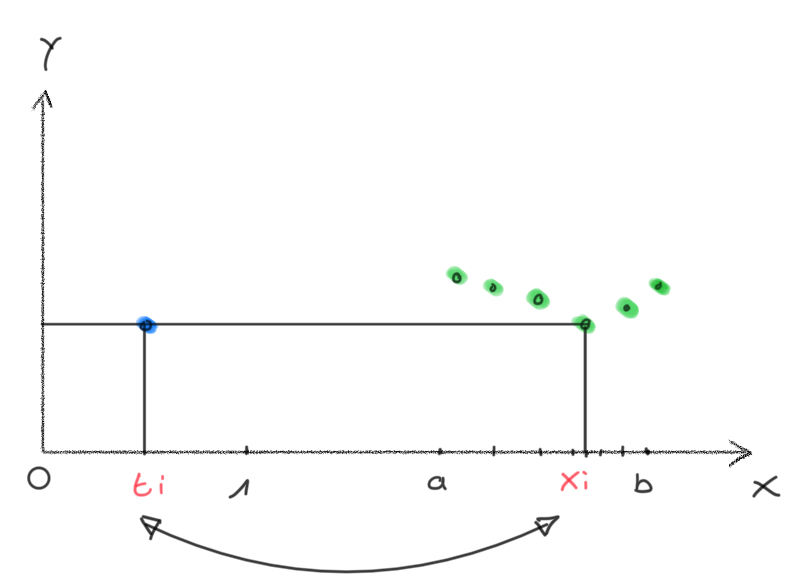
\includegraphics[width=0.5\linewidth]{bernstein_interpolation}
\end{center}
Ora il problema consiste nell'interpolare i punti $(t_i,y_i),i=0,\ldots,n$ con
un polinomio definito nella base di Bernstein:
$$p(t)=\displaystyle\sum_{i=0}^{n}c_iB_{in}(t)\quad \text{ con }t\in[0,1]$$
Imponendo le condizioni di esistenza, otteniamo un sistema lineare con la
stessa matrice, ma valutata nei punti $t_i=0,\ldots,n$ invece che $x_i$.
Questa rappresentazione consente di ottenere gli stessi coefficienti $c_i$ che
si otterrebbero lavorando in $[a,b]$, ma con una maggiore precisione, in
quanto meno suscettibile a problemi numerici.

Per la soluzione del sistema lineare si può applicare un algoritmo ad hoc
perché la matrice è \underline{totalmente positiva}, e perciò qualunque
sottomatrice presa quadrata che noi ritagliamo da questa avrà il determinante
$>0$. Per matrici fatte così esistono algoritmi efficienti per trovare una
soluzione con complessità $\mathcal{O}(n^2)$.
\subsubsection{Base di Lagrange}
Sia il metodo di Newton che il metodo di Bernstein, l'interpolazione richiede
la soluzione di un sistema lineare. Esiste però un metodo di interpolazione
che elimini completamente la necessità di risolvere un sistema lineare? 

Supponiamo di avere un insieme di punti $(x_i,y_i)$ e vogliamo trovare un
polinomio $p(x)\in \mathbb{P}_n$ che li interpoli. 

Anziché risolvere il problema di interpolazione su tutti i dati, possiamo
semplificarlo \underline{costruendo} un polinomio che ha zeri in tutti i punti
$x_i$, tranne in uno specifico punto $x_j$, dove vogliamo che il polinomio
valga 1. Per il Teorema \ref{eq:teorema_fondamentale_algebra}, i polinomi
$L_{i,n}(x)$ avendo come radici i punti $x_j$ con $j=0,\ldots,n$ e $j\neq i$
saranno nella forma
$$L_{i,n}(x)=d_i(x-x_0)(x-x_1)\cdots(x-x_{i-1})(x-x_{i+1})\cdots(x-x_n)$$ con
$d_i$ una costante da determinare in modo che $L_{i,n}(x_i)=1$. Troviamo $d_i$
come:
\begin{equation*}
   \begin{aligned}
       d_i(x_i-x_0)(x_i-x_1)\cdots(x_i-x_{i-1})(x_i-x_{i+1})\cdots(x_i-x_n)=1\\ 
       d_i=\frac{1}{(x_i-x_0)(x_i-x_1)\cdots(x_i-x_{i-1})(x_i-x_{i+1})\cdots(x_i-x_n)}\\ 
   \end{aligned}
\end{equation*}
da cui in definitiva
\begin{equation*}
   \begin{aligned}
       L_{i,n}(x)=&\frac{(x-x_0)(x-x_1)\cdots(x-x_{i-1})(x-x_{i+1})\cdots(x-x_n)}{(x_i-x_0)(x_i-x_1)\cdots(x_i-x_{i-1})(x_i-x_{i+1})\cdots(x_i-x_n)}
       \\ 
       &=\frac{\prod_{j=0,j\neq i}^n(x-x_j)}{\prod_{j=0,j\neq
       i}(x_i-x_j)}\quad i=0,\ldots,n
   \end{aligned} 
\end{equation*}
Sono $n+1$ funzioni che formano una base polinomiale per lo spazio
$\mathbb{P}_n$ detta base di Lagrange.
$$\left\{L_{0,n}(x),L_{1,n}(x),\ldots,L_{n,n}(x)\right\}\in \mathbb{P}_ n$$
Ora che abbiamo questi polinomi base di Lagrange, il problema è banalmente
risolto da 
\begin{equation}\label{eq:polinomio_forma_lagrange}
    \begin{aligned}
        p(x)=\displaystyle\sum_{i=0}^{n}y_iL_{i,n}(x)
    \end{aligned}
\end{equation}
infatti per le condizioni $L_{i,j}(x_j)=\begin{cases}
    1 & \text{se }i=j\\ 
    0 & \text{altrimenti}
\end{cases}$ che definiscono i polinomi $L_{i,n}(x)$,
banalmente in ogni punto $x_j$ l'espressione polinomiale
\ref{eq:polinomio_forma_lagrange} varrà $y_j$ per ogni $j=0,\ldots,n$.

Dal punto di vista computazionale determinare tale polinomio non costa
\underline{nulla}, essendo i coefficienti del polinomio in tale base proprio i
valori $y_i$ assegnati. Al contrario la valutazione del polinomio interpolante
comporta la determinazione e la valutazione dei polinomi $L_{i,n}(x)$.
\paragraph{Valutazione di un polinomio nella base di Lagrange.}
Calcolare i polinomi base di Lagrange può essere costoso, ma possiamo
semplificarlo utilizzando una formula alternativa.
\begin{itemize}
    \item [\textbf{I}] \textbf{forma baricentrica}:\\
        Iniziamo con il polinomio di Lagrange:
        $$L_{i,n}(x)=d_i\prod_{j=0,j\neq i}^n(x-x_j)$$
        dove $d_i=\frac{1}{\prod_{j=0,j\neq i}(x_i-x_j)}$

        Possiamo calcolare \underline{una volta sola} prima di valutare il polinomio:
        $$p(\bar{x})=\displaystyle\sum_{i=0}^{n}y_iL_{i,n}(\bar{x})$$
        Successivamente, determiniamo:
        $$l(x)=(x-x_0)(x-x_1)\cdots(x-x_n)$$
        cioè, il prodotto di tutti i termini senza saltarne nessuno e
        riscriviamo il polinomio di Lagrange come:
        $$L_{i,n}(x)=d_i \frac{l(x)}{x-x_i}$$
        Da cui segue:
        $$p(x)=\displaystyle\sum_{i=0}^{n}y_i \frac{w_il(x)}{x-x_i}$$
        Poiché $l(x)$ non dipende più dall'indice di sommatoria, possiamo
        portarlo fuori:
        $$l(x)\displaystyle\sum_{i=0}^{n}y_i \frac{w_i}{x-x_i}$$
        dove $w_i$ e $l(x)$ vengono calcolati una sola volta con $n$
        moltiplicazioni, e all'interno della sommatoria vengono effettuate 2
        moltiplicazioni per $n$ volte. Il costo computazionale totale per la
        valutazione è quindi $\mathcal{O}(n)$.
    \item [\textbf{II}] \textbf{forma baricentrica}:\\ 
        Consideriamo il polinomio nella forma di Lagrange che interpola $(x_i,
        y_i=1)$ per $i=0,\ldots,n$. Essendo la funzione costante $1$ l'unica
        che interpola i nostri dati in $\mathbb{P}_n$, allora  il polinomio
        nella I forma di Lagrange corrispondente a 1, è dato da:
        \begin{equation}\label{eq:lagrange_1}
           \begin{aligned}
               p(x)=l(x)\displaystyle\sum_{i=0}^{n}\frac{d_i}{x-x_i}1=1
           \end{aligned} 
        \end{equation}
        \begin{center}
            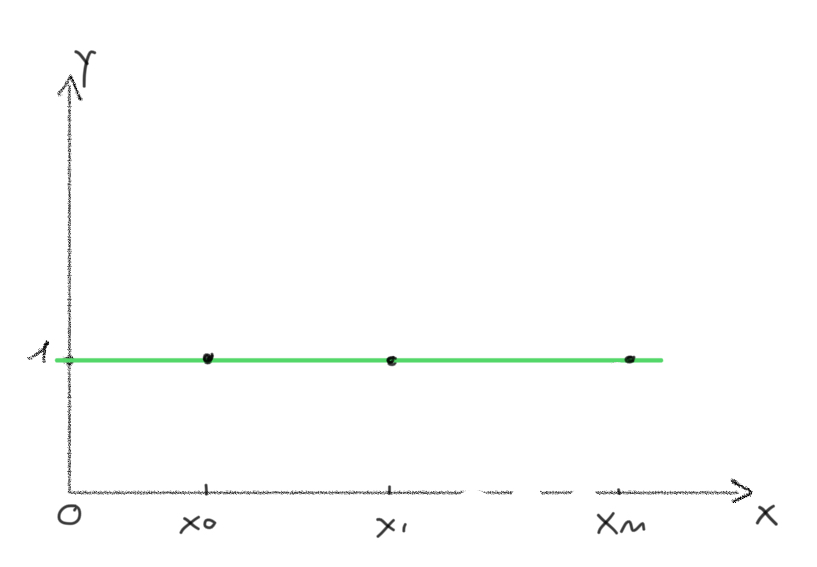
\includegraphics[width=0.4\linewidth]{lagrange_2_form}
        \end{center}
        Ora, dividendo la I forma di Lagrange per 1, ma scrivendo 1 come in
        \ref{eq:lagrange_1}, otteniamo: 
        \begin{equation*}
           \begin{aligned}
               p(x)=\frac{\cancel{l(x)}\displaystyle\sum_{i=0}^{n}y_i
                   \frac{d_i}{x-x_i}}{\cancel{l(x)} \displaystyle\sum_{i=0}^{n}
           \frac{d_i}{x-x_i}}
           \end{aligned} 
        \end{equation*}
        Il vantaggio di questa rappresentazione deriva dal fatto che,
        avendo semplificato analiticamente
        $l(x)$, non è più necessario calcolarlo. Il costo computazionale
        rimane $\mathcal{O}(n)$, ma con meno operazioni da fare, e si svolge come segue:
        \begin{itemize}
            \item Nel ciclo, si eseguono una divisione e una moltiplicazione
                al numeratore.
            \item Dopo il ciclo, si effettua un'ultima divisione.
        \end{itemize}
        Questo rende l'algoritmo più efficiente e \underline{altamente stabile
        numericamente}.
\end{itemize}
\begin{lstlisting}[language=Python]
def calculate_di(x, i):
    return 1/np.prod([x[i] - x[j] for j in range(len(x)) if j != i])

def lagrange_evaluation(x, y, x_bar):
    n = len(x)
    d = [calculate_di(x, i) for i in range(n)]
    
    num = 0
    den = 0
    for i in range(n):
        div = d[i]/(x_bar-x[i])
        num += y[i] * div
        den += div
    return num/den
\end{lstlisting}
\subsection{Errore di interpolazione (interpolazione di funzioni)}
\begin{recap}
    I termini \( C^k \) dove \( k \) è un intero non negativo, sono utilizzati per classificare le funzioni in base alla loro regolarità. Nello specifico:
    \begin{itemize}
        \item \( C^0 \): La funzione è continua.
        \item \( C^1 \): La funzione ha una derivata prima continua.
        \item \( C^2 \): La funzione ha derivate prima e seconda continue.
        \item \( \vdots \)
        \item \( C^\infty \): La funzione è infinitamente differenziabile e tutte le sue derivate sono continue.
    \end{itemize}
    Queste notazioni sono utilizzate per indicare quanto sia ``liscia" una funzione, cioè quante derivate continue possiede.
\end{recap}
Sia $f(x)$ è la funzione assegnata nell'intervallo $[a,b]$ e sia $p(x)$ il
polinomio interpolante nei punti $(x_i,f(x_i)),i=0,\ldots,n$; ha senso chiedersi quanto sia grande l'errore di
interpolazione
$$R(x)=\left\lvert f(x)-p(x)\right\rvert$$
che si commette in un punto $\bar{x}\in[a,b]$ diverso dai punti di
interpolazione $x_i$.
\begin{theorem}
    Sia $f(x)\in C_{[a,b]}^{(n+1)}$; siano $x_0,x_1,\ldots,x_n\in[a,b]$ punti
    di interpolazione distinti allora esiste un punto $\xi$ che dipende da
    $\bar{x}$ (punto di valutazione) per cui 
    \begin{equation}\label{eq:errore_interpolazione}
        \begin{aligned}
            f(\bar{x})=p(\bar{x})+{\color{red}\frac{w(\bar{x})}{(n+1)!}f^{(n+1)}(\xi)}
        \end{aligned}
    \end{equation}
    con $w(\bar{x})=(\bar{x}-x_0)(\bar{x}-x_1)\cdots(\bar{x}-x_n)$.
\end{theorem}
La parte evidenziata in {\color{red}rosso} rappresenta l'errore di interpolazione. Questa
quantità ci mostra come l'errore dipende dalla regolarità della funzione
($(n+1)$-esima derivata), dai punti interpolanti scelti, e dal punto di
valutazione $\bar{x}$ specifico.
\begin{example}
    Sia $f(x)=e^x$ con $x\in[a,b]$. Si osserva che:
    \begin{itemize}
        \item $\left\lvert f^{(n+1)}(\xi)\right\rvert\leq e^b$
        \item $w(\bar{x})=(\bar{x}-x_0)(\bar{x}-x_1)\cdots(\bar{x}-x_n)\leq(b-a)(b-a)\ldots(b-a)=(b-a)^{n+1}$
    \end{itemize}
    da cui 
    $$R(x)\leq
    \frac{(b-a)^{n+1}}{(n+1)!}e^{b}\underset{n\rightarrow\infty}{\to}0$$
    Notiamo che il fattore $(n+1)!$ cresce più velocemente di $(b-a)^{n+1}$, e
    quindi l'intero fattore tende a zero quando $n$ tende all'infinito.

    Questo dimostra che il polinomio interpolante converge alla funzione
    all'aumentare del numero dei punti di interpolazione.
    \begin{center}
        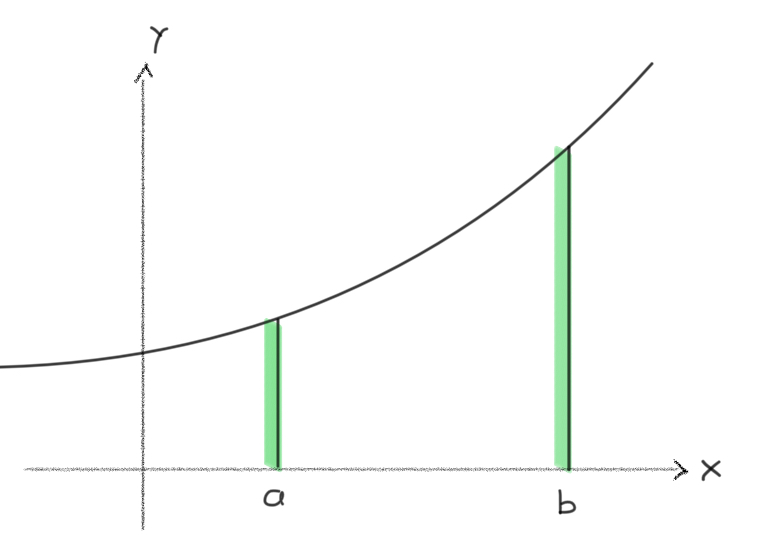
\includegraphics[width=0.4\linewidth]{e_x}
    \end{center}
\end{example}
\subsubsection{Punti equispaziati e di Chebyshev} Consideriamo la funzione
$f(x)=\frac{1}{1+x^2}$, definita sull'intervallo $x\in[-5,5]$, 
e il polinomio di interpolazione costruito utilizzando $n+1$ punti
\underline{equispaziati} $x_i=\frac{10}{n}i-5\quad i=0,\ldots,n$. 

Il matematico Runge dimostrò un caso in cui l'errore di interpolazione non
migliora, ma peggiora all'aumentare dei punti. Invece di convergere alla
funzione, il polinomio inizia ad oscillare vicino agli estremi
dell'intervallo, e queste oscillazioni si intensificano all'aumentare del numero di
punti in cui vado ad interpolare e del grado del polinomio che vado ad
utilizzare.

La causa di questo comportamento risiede proprio nella scelta dei punti
equispaziati.
\begin{figure}[ht]
    \centering
    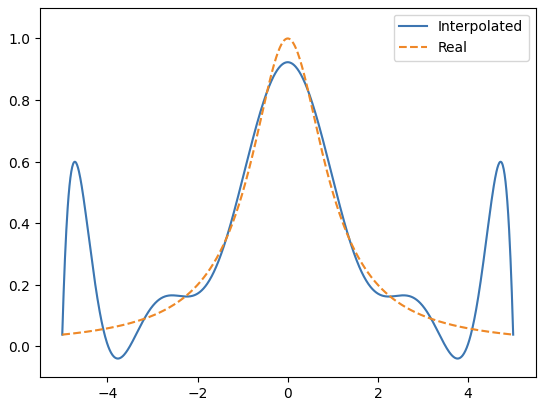
\includegraphics[width=0.5\linewidth]{runge}
    \caption{Interpolazione polinomiale della funzione di Runge su 11 punti
    equispaziati}
\end{figure}
\begin{theorem}
    Sia $I\in[-1,1]$ e i punti di interpolazione siano gli zeri del polinomio
    di Chebyshev di grado $n+1$.

    Se $f(x)\in C_{I}^0$ e soddisfa la condizione di Lipschitz\footnote{
        La condizione di Lipschitz richiede che la funzione non abbia
        variazioni troppo brusche tra due punti vicini, aiutando a garantire
        la regolarità della funzione.
    }
    $$\left\lvert f(\bar{x}-f(\tilde{x}))\right\rvert< K \left\lvert
    \bar{x}-\tilde{x}\right\rvert$$
    allora il polinomio interpolante converge uniformemente a $f(x)$ su $I$
    per $n\to\infty$ e $\left\lvert
    f(x)-p_n(x)\right\rvert\underset{n\rightarrow\infty}{\to}0$
\end{theorem}
Quindi se i punti di interpolazione vengono sono scelti opportunamente (come per esempio
gli zeri del polinomio di Chebyshev di grado $n+1$\footnote{
    $x_i=\cos(\frac{(2i+1)\pi}{2(n+1)}),\quad i=0,\ldots,n$ sono gli $n+1$
    zeri reali del polinomio di Chebyshev di prima specie di grado $n+1$
    definito in $[-1,1]$; se i punti di interpolazione sono in $[a,b]$ si
    applichi un mapping degli zeri da $[-1,1]$ in $[a,b]$
}) e la funzione $f(x)$ è Lipschitziana si ha la convergenza dell'interpolante
polinomiale. Più la $f$ è regolare e più veloce la convergenza.
\begin{figure}[ht]
    \centering
    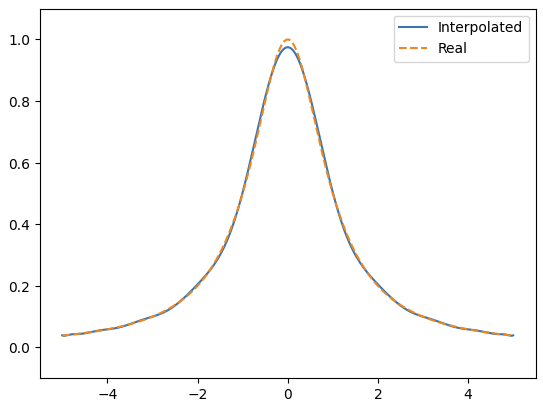
\includegraphics[width=0.5\linewidth]{chebyshev}
    \caption{Interpolazione polinomiale della funzione di Runge su 21 punti zeri
    di Chebyshev}
\end{figure}
\subsection{Interpolazione polinomiale a tratti}
I polinomi non sono sufficientemente flessibili per approssimare funzioni che
hanno differenti andamenti in differenti parti dell'intervallo di
definizione. Se si usa un polinomio di grado basso, questo 
approssima bene le parti lisce della funzione ma fallisce nel rappresentare
le parti più variabili. Al contrario, aumentando il grado del polinomio, si
ottiene una buona approssimazione delle parti più variabili, ma ciò 
potrebbe causare un comportamento oscillante nelle regioni in cui la funzione
è più liscia.

\begin{center}
    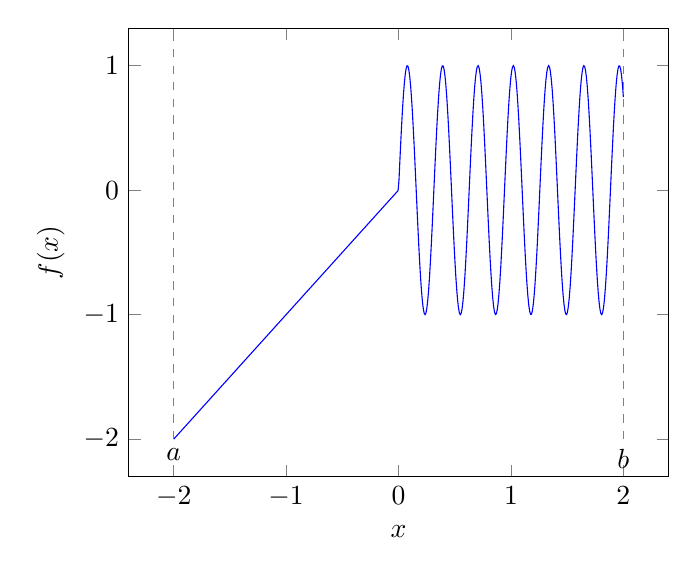
\begin{tikzpicture}
        \begin{axis}[
            xlabel=\(x\),
            ylabel={\(f(x)\)},
            legend pos=outer north east,
            domain=-2:2,
            samples=500
            ]

            % Funzione regolare seguita da un'oscillazione
            \addplot[blue] {x < 0 ? x : sin(20*deg(x))};

            % Linee verticali per l'intervallo [a,b]
            \draw [dashed, gray] (axis cs: -2, -2) -- (axis cs: -2, 2);
            \draw [dashed, gray] (axis cs: 2, -2) -- (axis cs: 2, 2);

            \node [below] at (axis cs: -2, -2) {\(a\)};
            \node [below] at (axis cs: 2, -2) {\(b\)};

        \end{axis}
    \end{tikzpicture}
\end{center}
Una soluzione a questo problema è utilizzare la classe dei polinomi a tratti.
\begin{definition}
    Sia $[a,b]$ un intervallo e siano$\left\{x_i\right\}_{i=1,\ldots,m-1}$ punti
    distinti e crescenti dell'intervallo $[a,b]$, cioè
    $$a=x_0<x_1<x_2<\ldots<x_m-1<x_m=b$$
    Questa sequenza di punti forma una \underline{partizione} dell'intervallo $[a,b]$ in
    $m$ sottointervalli. Allora si definisce un polinomio a tratti la
    funzione:
    $$pp(x)=\begin{cases}
        p_0(x) & x \in[x_0,x_1]\\
        p_1(x) & x \in[x_1,x_2]\\
        \vdots \\
        p_{m-1}(x) & x \in[x_{m-1},x_m]
    \end{cases}$$
\end{definition}
\begin{center}
    \begin{tikzpicture}
        \begin{axis}[
            xlabel=\(x\),
            ylabel={\(y\)},
            legend pos=north west,
            domain=-1:1,
            samples=100,
            ]

            \addplot[blue, domain=-1:-0.5] {x^2};
            \addplot[blue, only marks] coordinates {(-1,1) (-0.5,0.25)};

            \addplot[red, domain=-0.5:0] {-x^3};
            \addplot[red, only marks] coordinates {(-0.5, 0.125) (0,0)};

            \addplot[green, domain=0:0.5] {x^3};
            \addplot[green, only marks] coordinates {(0,0) (0.5,0.125)};

            \addplot[brown, domain=0.5:1] {-x^2};
            \addplot[brown, only marks] coordinates {(0.5,-0.25) (1,-1)};

            \draw [dashed, gray] (axis cs: -1, -1) -- (axis cs: -1, 2);
            \draw [dashed, gray] (axis cs: 1, -1) -- (axis cs: 1, 2);

            \node [below] at (axis cs: -1, -1) {\(a\)};
            \node [below] at (axis cs: 1, -1) {\(b\)};
        \end{axis}
    \end{tikzpicture}
\end{center}
Questa classe di polinomi risolve il problema dell'inflessibilità nella
rappresentazione delle funzioni. Consente di partizionare un
intervallo in sottointervalli e di utilizzare polinomi distinti per ciascun
sottointervallo. In questo modo, si può  adattare la rappresentazione ai vari comportamenti
della funzione all'interno dell'intervallo complessivo.

Tuttavia, questa soluzione introduce un problema di discontinuità nei nodi,
cioè nei punti in cui i sottointervalli si congiungono. Questa discontinuità
può essere problematica quando si vuole ricostruire una funzione che dovrebbe
essere regolare. 

Per risolvere questo problema, imponiamo delle \textsc{condizioni di
continuità} nei nodi. In altre parole, si può richiedere che i polinomi nei
tratti interni si accordino di valore
$$p_{i-1}(x)\equiv p_i(x)\quad i=i,\ldots,m-1$$
Oltre a ciò, possiamo imporre che le derivate $\ell$-esime si accordino di
valore nei nodi. In questo modo, si ottiene un certo ordine di continuità
$C^{l}$, che garantisce maggiore regolarità.
$$p^{(\ell)}_{i-1}(x)\equiv p_{i}^{(\ell)}\quad i=i,\ldots,m-1\text{ e }\ell=1,\ldots,n-1$$
Quando $\ell=n-1$ si ha la massima regolarità e la funzione polinomiale a
tratti viene chiamata funzione \textbf{spline}.
\vskip 0.1in
Con interpolazione polinomiale a tratti si intende l'interpolazione di un set
di dati in un intervallo $[a,b]$ con una funzione polinomiale a tratti. In
particolare, siano assegnati $m+1$ punti distinti e ordinati, cioè siano
assegnati $(x_i,y_i)\ i=0,\ldots,m$ con $x_i<x_{i+1}\ \forall i$. L'intervallo
$[a,b]$ è il più piccolo intervallo che contiene questi punti, quindi avremo $a=x_0$ e
$b=x_{m}$. 

Utilizziamo i punti di interpolazione $x_i$ per partizionare l'intervallo
$[a,b]$ in sottointervalli:

\begin{center}
    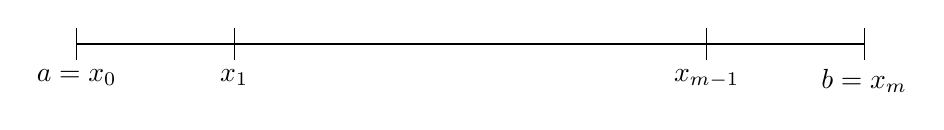
\begin{tikzpicture}
        \draw (0,0) -- (10,0);

        \foreach \x/\label in {0/{$a=x_0$}, 2/{$x_1$}, 8/{$x_{m-1}$}, 10/{$b=x_m$}}
        {
            \draw (\x,-0.2) -- (\x,0.2);
            \node[below] at (\x,-0.2) {\label};
        }
    \end{tikzpicture}
\end{center}

Definiamo un polinomio a tratti come segue:
$$pp(x)=\begin{cases}
    p_0(x) & x\in[x_0,x_1]\\
    \vdots \\
    p_{m-1}(x) & x\in[x_{m-1},x_m]
\end{cases}$$
Successivamente, imponiamo le condizioni di interpolazione $pp(x_i)=y_i,i=0\ldots,m$:
\begin{equation*}
    \begin{array}{ccc}
        p_0(x_0) = y_0, & \ldots, & p_{m-1}(x_m) = y_m
    \end{array}
\end{equation*}
\begin{example}
    Siano dati $(x_i,y_i)_{i=0,\ldots,2}=\left\{(1,1),(2,2),(3,1)\right\}$.
    Scegliamo $p(x)\in \mathbb{P}_1$, cioè un polinomio di grado 1 per
    ciascuno degli intervalli $[x_0,x_1]$ e $[x_1,x_2]$. Per farlo,
    utilizziamo la formula per un polinomio lineare tra due punti.
    \begin{center}
        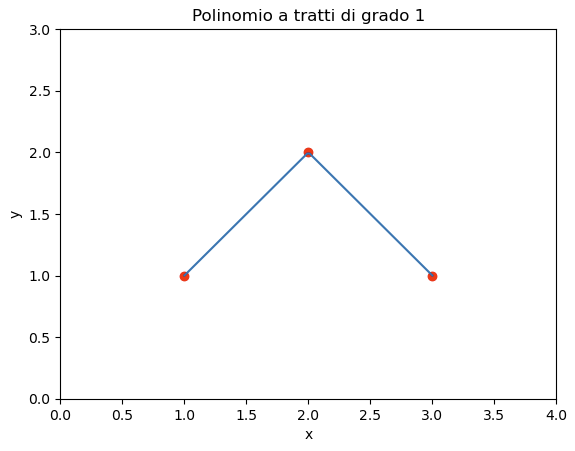
\includegraphics[width=0.6\linewidth]{piecewise_polynomial}
    \end{center}
\end{example}
\subsection{Condizionamento dell'interpolazione (interpolazione di funzioni)}
L'uso della forma di Lagrange per il polinomio interpolante è molto comoda per
analizzare l'errore inerente associato a questo problema.

Consideriamo il polinomio interpolante nella forma di Lagrange:
$$p(x)=\displaystyle\sum_{i=0}^{n}f(x_i)L_{i,n}(x)$$
Nell'analisi del condizionamento di questo problema, dobbiamo identificare
i dati  coinvolti. Poiché gli $x_i$ sono numeri finiti scelti da noi, non sono
soggetti a errori di approssimazione. L'errore potrebbe verificarsi nel 
valore della funzione $f$, dato che potrebbe essere rappresentato in modo
approssimato.

Supponiamo ora che gli $f(x_i)$ siano perturbati da una quantità $\delta
f(x_i)$, e denotiamo le valutazioni della funzione perturbate come:
$$\hat{f}(x_i)=f(x_i)+\delta f(x_i)$$ 
Di conseguenza, il polinomio perturbato sarà:
\begin{equation*}
   \begin{aligned}
       \hat{p}(x)=\displaystyle\sum_{i=0}^{n}\hat{f}L_{i,n}(x)
   \end{aligned} 
\end{equation*}
L'errore inerente in questo caso consiste nel valutare la differenza tra
$p(x)$ e $\hat{p}(x)$, ovvero tra il polinomio calcolato con i dati esatti e
il polinomio calcolato con i dati perturbati.
\begin{equation*}
   \begin{aligned}
       \left\lvert \hat{p}(x)-p(x)\right\rvert &=\left\lvert
           \displaystyle\sum_{i=0}^{n}(f(x_i)+\delta
       f(x_i))L_{i,n}(x)-\displaystyle\sum_{i=0}^{n}f(x_i)L_{i,n}(x)\right\rvert\\ 
                         &= \left\lvert \displaystyle\sum_{i=0}^{n}\delta
                         f(x_i)L_{i,n}(x)\right\rvert\\
                         &\leq \displaystyle\sum_{i=0}^{n} \left\lvert \delta
                         f(x_i)\right\rvert \left\lvert
                         L_{i,n}(x)\right\rvert\\ 
                         &\leq \max_{0\leq i\leq n}\left\lvert \delta
                         f(x_i)\right\rvert
                         {\color{red}\displaystyle\sum_{i=0}^{n}\left\lvert
                         L_{i,n}(x)\right\rvert}
   \end{aligned} 
\end{equation*}
Definiamo il numero di condizione del problema di interpolazione nel punto $x$
come:
$$C_{\text{Int}}(p(x))=\displaystyle\sum_{i=0}^{n}\left\lvert L_{i,n}(x)\right\rvert$$
Il massimo numero di condizione su tutto il dominio $X$ sarà quindi:
$$\Lambda_n(X)=\max_{x\in X} C_{\text{Int}}(p(x))\quad \text{ con }X=\left\{
    x_0,x_1,\ldots,x_n
\right\}$$
Questa è chiamata \textbf{costante di Lesbegue}. Se la costante è dell'ordine
di $\log(n)$, allora il problema è ben condizionato; altrimenti, è mal
condizionato.
\newpage
\section{Integrazione numerica}
\begin{theorem}[Teorema fondamentale del calcolo integrale]
    Sia $f: [a,b]\rightarrow \mathbb{R}$ una funzione integrabile. Supponiamo
    che $f$ abbia una primitiva $F:[a,b]\rightarrow \mathbb{R}$. Allora
    $$\displaystyle\int_{a}^{b}f(x)\ dx=F(b)-F(a)=F(x)\big|_{x=a}^b$$
\end{theorem}
Questo teorema afferma che il calcolo di un integrale può essere semplificato
trovando una primitiva della funzione e valutandola agli estremi
dell'intervallo. È importante notare, però, che non tutte le funzioni
possiedono una primitiva. 
\begin{example}
   $$\int_{0}^{1}x\ dx=\frac{1}{2}x^2\bigg|_{x=0}^{1}=\frac{1}{2}$$ 
   $$\int_{0}^{1}e^x\ dx=e^x \big|_{x=0}^{1}=e-1$$
\end{example}
Se la funzione da integrare è difficile da risolvere analiticamente, non
possiede una primitiva o è irrazionale, l'approccio rimanente è quello di
procedere numericamente calcolando un valore approssimato del suo integrale. 

L'idea dietro all'integrazione numerica  consiste nell'approssimare la
funzione $f(x)$ con un polinomio ottenuto tramite l'interpolazione
polinomiale. Questo polinomio interpolante viene poi integrato nell'intervallo
$[a,b]$ per ottenere un'approssimazione del valore dell'integrale.
\begin{center}
    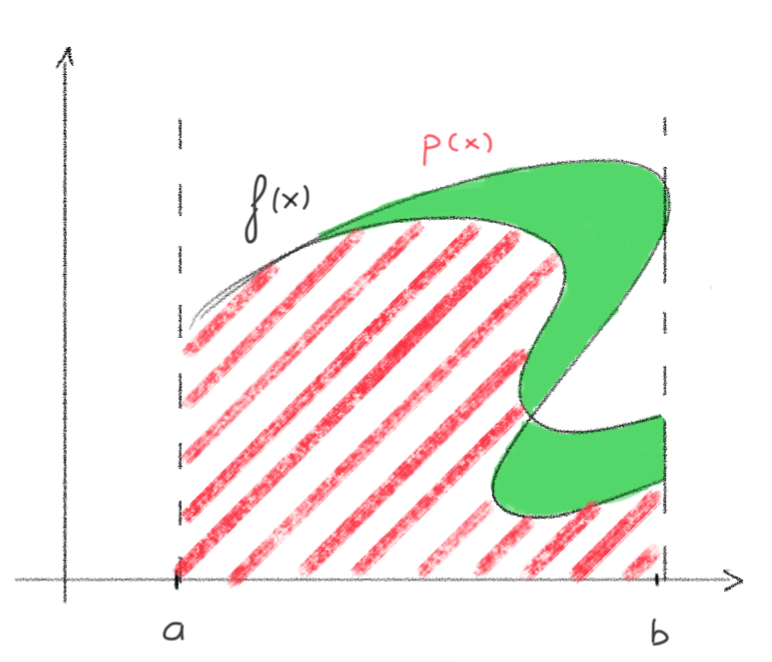
\includegraphics[width=0.45\linewidth]{integral_error}
\end{center}
Poiché l'integrazione viene effettuata su un approssimazione polinomiale, si
introduce inevitabilmente un errore. Questo errore si manifesta come aree in
eccesso o in difetto, che contribuiscono all'errore rispetto al risultato
finale.
$$\displaystyle\int_{a}^{b}f(x)\ dx= \displaystyle\int_{a}^{b}p(x)\
dx+\text{errore}\approx \displaystyle\int_{a}^{b}p(x)\ dx$$
\subsection{Formule di quadratura di Newton-Cotes}
Scegliamo $n+1$ punti di interpolazione $x_i$ \underline{equispaziati}
nell'intervallo $[a,b]$. Questi punti sono dati da: $$x_i=a+ih\quad
i=0,\ldots,n\quad\text{con}\quad h=\frac{b-a}{n}\quad\text{per}\quad n>0$$
Successivamente, costruiamo un polinomio interpolante $p\in \mathbb{P}_n$ sui
punti $(x_i,f(x_i))_{i=0,\ldots,n}$. Questo polinomio è espresso nella forma
di Lagrange:
$$p(x)=\displaystyle\sum_{i=0}^{n}f(x_i)L_{i,n}(x)$$
Per approssimare l'integrale di $f(x)$ sull'intervallo $[a,b]$, possiamo
sostituire la funzione integranda $f(x)$ con il polinomio interpolante $p(x)$:
\begin{equation*}
    \begin{aligned}
        \displaystyle\int_{a}^{b}f(x)\ dx\approx
        \displaystyle\int_{a}^{b}p(x)\ dx&=\displaystyle\int_{a}^{b}\displaystyle\sum_{i=0}^{n}f(x_i)L_{i,n}(x)\
        dx \\
        \alignedintertext{Applicando la proprietà che l'integrale della somma
        è la somma degli integrali e notando che $f(x_i)$ è una costante
    rispetto all'integrazione, otteniamo:}\\
                                         &=\displaystyle\sum_{i=0}^{n}f(x_i)\displaystyle\int_{a}^{b}L_{i,n}(x)\
        dx \\
        \alignedintertext{Definiamo ora gli
        integrali dei polinomi di Lagrange su $[a,b]$ come i coefficienti $w_i$:}
                                         &=\displaystyle\sum_{i=0}^{n}f(x_i)w_i
    \end{aligned}
\end{equation*}
Questa è la \textbf{formula di quadratura}, una combinazione lineare della
funzione $f(x)$ pesata dai coefficienti $w_i$. Procediamo alla loro
integrazione. 
\begin{equation*}
   \begin{aligned}
       \displaystyle\int_{a}^{b}L_{i,n}(x)\ dx&=\displaystyle\int_{a}^{b}\prod_{j=0,j\neq i}\frac{x-x_j}{x_i-x_j}\
       dx \\
       \alignedintertext{Effettuiamo un cambio di variabile di integrazione da
       $x\in[a,b]$ a $t\in[0,n]$ mediante la $x=a+ht$ con $h=\frac{b-a}{n}$}\\ 
                                              &=\displaystyle\int_{0}^{n}\prod_{j=0,j\neq
       i}\frac{\cancel{a}+\cancel{h}t-\cancel{a}-\cancel{h}j}{\cancel{a}+\cancel{h}i-\cancel{a}-\cancel{h}j}h\
       dt \\  
                                              &=h{\color{red}\displaystyle\int_{0}^{n}\prod_{j=0,j\neq
       i}\frac{t-j}{i-j}\ dt}\\ 
                                              &=h{\color{red}W_i}
   \end{aligned} 
\end{equation*}
Notiamo che che i coefficienti $W_i$, dipendono soltanto dal grado $n$ del
polinomio interpolante e non dalla specifica funzione $f(x)$  da integrare o
dall'intervallo di integrazione. Quindi, una volta calcolati, possono essere
utilizzati  per approssimare l'integrale di qualsiasi funzione $f(x)$ senza
doverli ricalcolare.
\subsubsection{Formula (dei Trapezi) per $n=1$}
Si procede al calcolo dei $W_i$ per $i=0,1$ (caso $n=1$).
$$W_0=\displaystyle\int_{0}^{1}\frac{t-1}{0-1}\
dt=\displaystyle\int_{0}^{1}1-t\ dt=\left(-\frac{t^2}{2}+t
\right)\bigg|_{x=0}^{1}=\frac{1}{2}$$

$$W_1=\displaystyle\int_{0}^{1}\frac{t-0}{1-0}\
dt=\displaystyle\int_{0}^{1}t\ dt=\frac{t^2}{2}
\bigg|_{x=0}^{1}=\frac{1}{2}$$
e quindi 
$$\displaystyle\int_{a}^{b}f(x)\
dx\approx\displaystyle\int_{a}^{b}p_1(x)=h
\displaystyle\sum_{i=0}^{1}f(x_i)W_i=\frac{h}{2}(f(x_0)+f(x_1))$$

\begin{figure}[!ht]
    \centering
    \begin{tikzpicture}
        \begin{axis}[
            axis lines=middle,
            xlabel=\(x\),
            ylabel=\(f(x)\),
            ymin=0,
            ymax=20,
            xmin=0,
            xmax=5,
            xtick={1,4},
            xticklabels={\(a\), \(b\)},
            samples=100
            ]
            % Funzione da integrare (es. f(x) = x^2)
            \addplot[blue, domain=1:4] {x^2};

            % Trapezio
            \draw[red, thick] (axis cs:1,1) -- (axis cs:4,16) -- (axis cs:4,0) -- (axis cs:1,0) -- cycle;
        \end{axis}
    \end{tikzpicture}
    \caption{Interpolazione lineare per formula dei trapezi}
\end{figure}
\newpage
\subsubsection{Formula (di Simpson) per $n=2$}
Si procede al calcolo dei $W_i$ per $i=0,1,2$ (caso $n=2$).

$$W_0=\displaystyle\int_{0}^{2}\frac{t-1}{0-1}\frac{t-2}{0-2}\
dt=\frac{1}{2}\displaystyle\int_{0}^{2}t^2-3t+2\
dt=\frac{1}{2}\left(\frac{t^3}{3}-\frac{t^2}{2}+2t
\right)\bigg|_{x=0}^{2}=\frac{1}{3}$$
$$W_1=\displaystyle\int_{0}^{2}\frac{t-0}{1-0}\frac{t-2}{1-2}\
dt=-\displaystyle\int_{0}^{2}t^2-2t\
dt=-\left(\frac{t^3}{3}-2\frac{t^2}{2}
\right)\bigg|_{x=0}^{2}=\frac{4}{3}$$
$$W_2=\displaystyle\int_{0}^{2}\frac{t-0}{2-0}\frac{t-1}{2-1}\
dt=\frac{1}{2}\displaystyle\int_{0}^{2}t^2-t\
dt=\frac{1}{2}\left(\frac{t^3}{3}-2\frac{t^2}{2}
\right)\bigg|_{x=0}^{2}=\frac{1}{3}$$
e quindi 
$$\displaystyle\int_{a}^{b}f(x)\
dx\approx\displaystyle\int_{a}^{b}p_2(x)=h
\displaystyle\sum_{i=0}^{2}f(x_i)W_i=\frac{h}{3}(f(x_0)+4f(x_1)+f(x_2))$$

\begin{figure}[!ht]
   \centering 
   \begin{tikzpicture}[scale=1.5]
       \draw[->] (-0.5,0) -- (4,0) node[right] {$x$};
       \draw[->] (0,-0.5) -- (0,2.5) node[above] {$y$};

       \draw[domain=0.2:3.8,smooth,variable=\x,blue] plot ({\x},{0.2*(\x-2)^3 + 0.5});
       \draw[domain=1.2:3.8,variable=\x,red] plot ({\x},{0.6*(\x-1.5)^2 + 0.2});

       \draw[red,thick] (1.5,0) -- (1.5,{0.6*(1.5-1.5)^2 + 0.2});
       \draw[red,thick] (3.5,0) -- (3.5,{0.6*(3.5-1.5)^2 + 0.2});

       \node[below] at (1.5,-0.15) {$a$};
       \node[below] at (2.5,-0.15) {$m$};
       \node[below] at (3.5,-0.15) {$b$};
   \end{tikzpicture}
   \caption{Interpolazione quadratica per formula di Simpson}
\end{figure}

\begin{example}
    Applichiamo le formule dei Trapezi e di Simpson per il calcolo di
    $\int_{0}^{1}e^{-x^2}\ dx$, che è un esempio di integrale non risolubile
    tramite il calcolo della funzione primitiva. Il valore esatto alle prime 6
    cifre significative è 0.746824.

    Applichiamo la formula dei Trapezi:
    $$\displaystyle\int_{0}^{1}e^{-x^2}\ dx\approx
    \frac{h}{2}(e^0+e^{-1})=0.683939.$$
    Applichiamo la formula di Simpson:
    $$\displaystyle\int_{0}^{1}e^{-x^2}\ dx\approx
    \frac{h}{3}(e^0)+4e^{-1/4}+e^{-1}=0.747180.$$
\end{example}
\subsubsection{Errore di integrazione}
\begin{table}[h]
\centering
\caption{Errore nell'Integrazione Numerica}
\begin{tabular}{|c|c|c|c|}
\hline
\( n \) & \( \sigma_i \) & \( s \) & \( R \) \\
\hline
1 & 1 1 & 2 & \(-\frac{1}{12} h^3 f^{(2)}(\eta)\) \\
\hline
2 & 1 4 1 & 3 & \(-\frac{1}{90} h^5 f^{(4)}(\eta)\) \\
\hline
3 & 1 3 3 1 & $\frac{8}{3}$ & $-\frac{3}{80}h^5f^{(4)}(\eta)$ \\
\hline
4 & 7 32 12 32 7 & $\frac{45}{9}$ & $-\frac{8}{945}h^7f^{(6)}(\eta)$ \\
\hline
\end{tabular}
\end{table}
\begin{definition} [Grado di precisione di una formula di quadratura]
    Una formula di quadratura si dice che ha grado di precisione $n$ se
    fornisce il valore esatto dell'integrale di grado $\leq n$.
\end{definition}
Per la formula dei Trapezi, il grado di precisione è 1, mentre per la formula
di Simpson il grado di precisione è 3.
\begin{oss}
    Si osserva che, mentre la formula dei trapezi, come ci si potrebbe
    aspettare è esatta per polinomi lineari di grado 1, la formula di Simpson
    rimane esatta non solo per polinomi di grado 2, come ci si
    aspetterebbe, ma anche per polinomi di grado 3. Questo avviene nonostante
    il fatto che un polinomio interpolante di grado 2 non dovrebbe, in teoria,
    essere in grado di rappresentare esattamente il polinomio di grado 3.
    Tuttavia, gli errori in eccesso e in difetto che si verificano si
    compensano esattamente, rendendo la formula esatta.

    La chiave sta nelle derivate: la derivata seconda di una funzione lineare
    è zero, e la derivata quarta di un polinomio di grado 2 o 3 è anche zero,
    annullando quindi l'errore.
    \begin{center}
        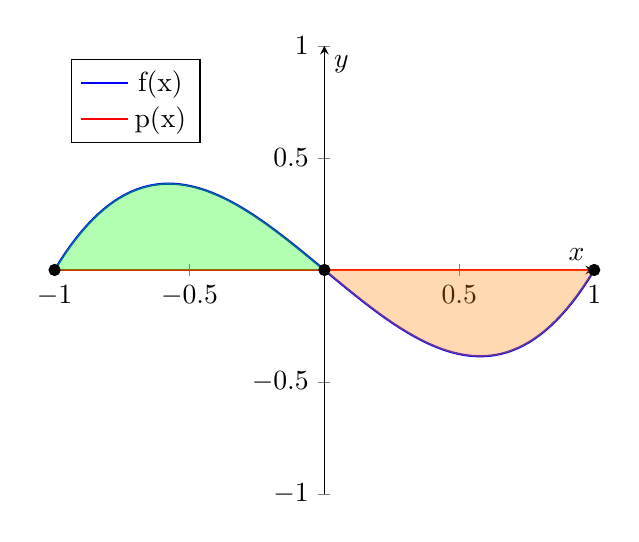
\begin{tikzpicture}
            \begin{axis}[
                axis lines = middle,
                xlabel = \(x\),
                ylabel = \(y\),
                domain = -1:1,
                samples = 100,
                legend pos = north west,
                ymin = -1,
                ymax = 1
                ]

                \addplot[blue, thick, domain=-1:1] {x^3 - x};
                \addlegendentry{f(x)}

                    \addplot[red, thick, domain=-1:1] {0};
                    \addlegendentry{p(x)}

                        \addplot[only marks] coordinates {(-1,0) (0,0) (1,0)};

                        \addplot[green, fill=green, opacity=0.3, domain=-1:0] {x^3 - x} \closedcycle;
                        \addplot[orange, fill=orange, opacity=0.3, domain=0:1] {x^3 - x)} \closedcycle;
                    \end{axis}
                \end{tikzpicture}
            \end{center}
    Questo comportamento si ha in tutte le formule con $n$ dispari ed $n$ pari
    rispettivamente.
\end{oss}
\begin{theorem}
    Il grado di precisione delle formule di Newton-Cotes è $n$ se $n$ è
    dispari, è $n+1$ se $n$ è pari.
\end{theorem}
Per $n\geq8$, le formule diventano instabili a causa dei
coefficienti di \underline{segno diverso} e dell'aumento del loro valore
assoluto che portano a problemi di cancellazione numerica e
perdita di precisione. Di conseguenza, si rende necessaria la ricerca di
formule più stabili e precise.
\subsection{Formule di quadratura composite}
Le formule composte consistono nel considerare dei polinomi a tratti come
funzioni approssimanti della funzione integranda nell'intervallo $[a,b]$.
$$\displaystyle\int_{a}^{b}f(x)\ dx\approx \displaystyle\int_{a}^{b}pp_1(x)\
dx$$
In pratica tale intervallo viene suddiviso in sottointervalli di
\underline{uguale ampiezza} ($h=\frac{b-a}{m}$), $[x_i,x_{i+1}]\
i=0,\ldots,m-1$, e su ciascuno di essi si applica una formula di quadratura.
La formula di quadratura composita è data dalla somma degli integrali
calcolati su tutti gli intervalli.
$$\displaystyle\int_{a}^{b}f(x)\ dx\approx \displaystyle\sum_{i=0}^{m-1}
\displaystyle\int_{x_i}^{x_{i+1}}p_{n}(x)\ dx$$
Al variare di $n$ abbiamo le varie formule composite:
\begin{itemize}
    \item \textbf{Formula dei Trapezi composita}:

            $\displaystyle\sum_{i=0}^{m-1}\displaystyle\int_{x_i}^{x_{i+1}}p_1(x)\
                dx=h(\frac{1}{2}f(x_0)+f(x_1)+\ldots+f(x_{m-1})+\frac{1}{2}f(x_m))+R_{TC}$
                \begin{center}
                    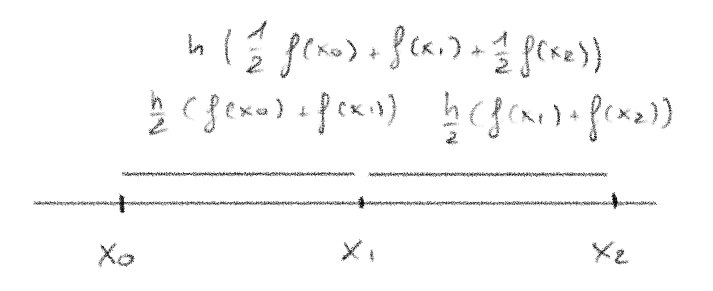
\includegraphics[width=0.4\linewidth]{tc_1.jpeg}
                \end{center}
                Dove $R_{TC}$ è definito come segue:
                \begin{equation}\label{eq:error_tc}
                   \begin{aligned}
                       R_{TC} &= -
                       \frac{h^3}{12}\displaystyle\sum_{i=0}^{m-1}f^{(2)}(\eta_i)
                              & \eta_i\in(x_i,x_{i+1})\\ 
                              \alignedintertext{Sostituendo $h=\frac{b-a}{m}$,
                              l'errore diventa:}
                              &=
                              -\frac{h^2}{12}(\frac{b-a}{\color{red}{m}}){\color{red}\displaystyle\sum_{i=0}^{m-1}f^{(2)}(\eta_i)}\\
                              \alignedintertext{La parte in
                              {\color{red}rosso} rappresenta una media dei
                          valori delle derivate seconde da 0 a $m-1$.
                          Utilizzando il \textsc{Teorema del valor medio}, questo termine è uguale alla
                  derivata seconda valutata in un opportuno punto $\eta$
              nell'intervallo $(a,b)$. Pertanto, possiamo riscrivere $R_{TC}$
          come segue:} \\ 
                             &= - \frac{b-a}{12}h^2f^{(2)}(\eta) & \eta
                             \in(a,b)
                   \end{aligned} 
                \end{equation}
                Poiché $h=\frac{b-a}{m}$, man mano che $m$ aumenta, $h$ diventa più
                piccolo, migliorando la precisione dell'integrale e riducendo
                l'errore. 
                $$R_{TC}\underset{m\to\infty}{\to}0$$
                Un vantaggio chiave dell'uso delle formule di
                quadratura composte, è proprio questo incremento di precisione
                quando si aumenta il numero di sottointervalli $m$. 
    \item \textbf{Formula di Simpson composita}:
        se prendiamo $m=2k$ l'intervallo $[a,b]$ viene diviso in un numero
        pari di sottointervalli. Ogni sottointervallo è delimitato dai punti
        $[x_{2i},x_{2i+2}]$ e include tre punti distinti. In questo modo,
        possiamo utilizzare la formula di Simpson per calcolare l'integrale in ogni
        sottointervallo.
        \begin{center}
            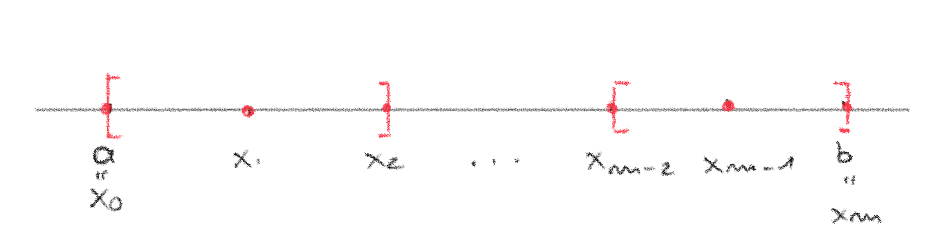
\includegraphics[width=0.5\linewidth]{sc_1}
        \end{center}

        $\displaystyle\sum_{i=0}^{k-1}\displaystyle\int_{x_{2i}}^{x_{2i+1}}p_2(x)\
        dx=\frac{h}{3}(f(x_0)+4f(x_1)+2f(x_2)+4f(x_3)+\ldots+f(x_m))+R_{SC}$

        Dove $R_{SC}$ è definito come segue:
        \begin{equation}\label{eq:error_sc}
           \begin{aligned}
               R_{SC}&=-\frac{h^5}{90}\displaystyle\sum_{i=0}^{k-1}f^{(4)}(\eta_i)
                     & \eta_i(x_{2i},x_{2i+1})
               \\ 
               \alignedintertext{Per le stesse argomentazione usate per la
               formula dei trapezi, questo si può scrivere:}\\
                     &=-\frac{h^4}{90}\frac{b-a}{{\color{red}2k}}{\color{red}\displaystyle\sum_{i=0}^{k-1}f^{(4)}(\eta_i)}\\
                     &=-\frac{b-a}{180}h^4f^{(4)}(\eta) & \eta\in(a,b)
           \end{aligned} 
        \end{equation}
        In questo caso, il valore di $h$ converge più rapidamente rispetto al
        metodi dei Trapezi composito quando si aumenta $m$.
\end{itemize}
\begin{example}
    Dato l'integrale
   $$\displaystyle\int_{0}^{1}\frac{1}{1+x}\ dx$$
   il cui valore esatto è 0.693147.

   Calcolare il valore approssimato dell'integrale e l'errore $R$ utilizzando sia la formula
   dei Trapezi composita che la formula di Simpson composita.
    
   \begin{center}
       \begin{tabular}{|r|c|c|c|c|}
           \hline
           \( h \) & \( T(h) \) & \( R_{\text{TC}} \) & \( S(h) \) & \( R_{\text{SC}} \) \\
           \hline
           \( h \)=1 & 0.75 & 0.0568 & - & - \\
           \( h/2 \)=0.5 & 0.708  & 0.01518  & 0.6944 &  0.00129 \\
           \( h/4 \)=0.25 &  0.697 & 0.0038  & 0.6932  & 0.000107 \\
           \( h/8 \)=0.125 &  0.694 & 0.0097  & 0.69315 & 0.00009 \\
           \hline
       \end{tabular}
   \end{center}

   Come visto precedentemente, l'errore \( R_{\text{TC}} \) nel metodo dei
   Trapezi composito è proporzionale a \( h^2 \), mentre l'errore \(
   R_{\text{SC}} \) nel metodo di Simpson composito è proporzionale a \( h^4
   \). Effettivamente, nell'esempio questo è confermato: il rapporto di
   riduzione dell'errore nel metodo dei Trapezi è di un fattore 4, mentre nel
   metodo di Simpson è di un fattore 16 quando \( h \) viene dimezzato.
\end{example}
\begin{example}
   Determinare il passo $h$ da utilizzare nella formula dei Trapezi composita
   e nella formula di Simpson composita, affinché
   l'integrale $\displaystyle\int_{0}^{1}\frac{1}{1+x}\ dx$ sia approssimato alla
   tolleranza $0.5\times 10^{-3}$.
   \vskip 0.1in
   Si considera la formula \ref{eq:error_tc} per l'errore di integrazione dei
   Trapezi composita e si cerca un limite superiore per la $f^{(2)}$ in
   $[a,b]$; nel caso specifico sarà:
   \begin{equation*} 
       \begin{aligned}
           & f'(x)=(1+x)^{-1} & f^{''}(x)=2(1+x)^{-3}
       \end{aligned}
   \end{equation*}
   Allora 
   $$\max_{0\leq x\leq 1}f^{''}(x)=f^{''}(0)=2$$
   e ricordando che $h=\frac{b-a}{2k}$ si ha:
   $$\left\lvert\frac{b-a}{12}h^2f^{''}(\eta) \right\lvert\leq 
           \frac{1}{\cancel{12}\
           6}h^2\cancel{2}=\frac{1}{6}\frac{1}{4k^2}=\frac{1}{24k^2}\leq 0.5\times10^{-3}$$
   da cui 
   $$k^2\geq \frac{2}{24}\times 10^3\quad \text{e quindi }k\geq9.12$$
   Segue che per approssimare l'integrale dato alla tolleranza fissata con il
   metodo dei Trapezi composito è sufficiente usare $k=10$, cioè il più
   piccolo intero che soddisfa $k\geq 9.12$.
   \vskip 0.1in
   Si considera la formula \ref{eq:error_sc} per l'errore di integrazione di
   Simpson composita e si cerca un limite superiore per la $f^{(4)}$ in
   $[a,b]$; nel caso specifico sarà:
   \begin{equation*} 
       \begin{aligned}
           & f^{(3)}(x)=6(1+x)^{-4} & f^{(4)}(x)=24(1+x)^{-5}
       \end{aligned}
   \end{equation*}
   Allora 
   $$\max_{0\leq x\leq 1}f^{(4)}(x)=f^{(4)}(0)=24$$
   si ha:
   $$\left\lvert\frac{b-a}{180}h^4f^{(4)}(\eta) \right\lvert\leq 
       \frac{1}{\cancel{180}\ 15}h^4 \cancel{24}\ 2=\frac{2}{15}\frac{1}{16k^4}=\frac{1}{120k^4}\leq 0.5\times10^{-3}$$
   da cui 
   $$k^4\geq \frac{2}{120}\times 10^3\quad \text{e quindi }k\geq2.0205$$
   Segue che per approssimare l'integrale dato alla tolleranza fissata con il
   metodo di Simpson composita è sufficiente usare $k=3$, cioè il più
   piccolo intero che soddisfa $k\geq 2.0205$.
\end{example}
\subsection{Metodi adattivi}
Si desidera che la differenza tra l'integrale esatto
$\displaystyle\int_{a}^{b}f(x)\ dx$ e la sua approssimazione $I_A$ sia
contenuta entro una certa tolleranza $tol$. 
$$\left\lvert \displaystyle\int_{a}^{b}f(x)\ dx- I_A\right\rvert\leq tol$$
Purtroppo, quando non si conosce il valore esatto dell'integrale, quanto visto
fino ad ora non permette di soddisfare questa richiesta.

Nella prossima sezione vedremo una tecnica nota come estrapolazione di
Richardson che permette di stimare numericamente l'errore di integrazione.
\subsubsection{Estrapolazione di Richardson}
Con \textbf{estrapolazione di Richardson} ci si riferisce ad una tecnica che
permette di ottenere dall'applicazione di due formule di integrazione composte
con passi rispettivamente $h$ ed $\frac{h}{2}$ un valore di approssimazione
per l'integrale più preciso dei due precedenti. Vediamo questa tecnica nel
caso delle formule composite:
\paragraph{Caso Trapezi.} 
\begin{corollary}
    Assumendo che la $f(x)$sia derivabile almeno 4 volte su $[a,b]$, si
    ha:
    $${\color{red}\displaystyle\int_{a}^{b}f(x)\ dx-T(h/2)\approx
    \frac{T(h/2)-T(h)}{3}+\mathcal{O}(h^4)}$$
    da cui 
    $${\color{green}\displaystyle\int_{a}^{b}f(x)\ dx\approx
    \frac{4T(h/2)-T(h)}{3}+\mathcal{O}(h^4)}$$
\end{corollary} 
\begin{oss}\leavevmode\
    \begin{itemize}
        \item[{\color{green}*}]\textbf{Miglioramento della stima}. Questo metodo consente di eliminare la potenza più bassa (2) 
            combinando opportunamente $T(h)$e $T(h/2)$, al fine di ottenere un'approssimazione
            più precisa dell'integrale.
        \item[{\color{red}*}]\textbf{Stima dell'errore}. Inoltre, il corollario fornisce una stima
            del termine principale dell'errore e quindi fornisce un metodo
            pratico per raggiungere l'obiettivo che si è posti. Si può
            progettare un metodo iterativo in cui si dimezza il passo fino
            a che 
            \begin{equation}\label{eq:stima_errore_integrazione}
                \left\lvert \frac{T(h/2)-T(h)}{3}\right\rvert\leq tol
            \end{equation} 
            quando questo si verifica, per il corollario, sarà anche 
            $$\left\lvert \displaystyle\int_{a}^{b}f(x)\
            dx-T(h/2)\right\rvert\leq tol$$
            e avremo una buona integrazione con $T(h/2)$. Questo metodo
            iterativo può essere applicato in modo adattivo. 
    \end{itemize}
\end{oss}
In un approccio adattivo il numero di punti viene scelto in base alla
regolarità della funzione. Si suddivide l'intervallo di integrazione,
\underline{solo dove serve}, in sottointervalli e si applica ricorsivamente a
questi una formula di quadratura sfruttando la stima dell'errore di
integrazione \ref{eq:stima_errore_integrazione} per il test di arresto. La
funzione integranda viene così valutata in pochi punti nei sottointervalli in
cui ha un andamento regolare e in molti punti negli intervalli dove sono
presenti irregolarità.
\begin{figure}[ht]
    \centering
    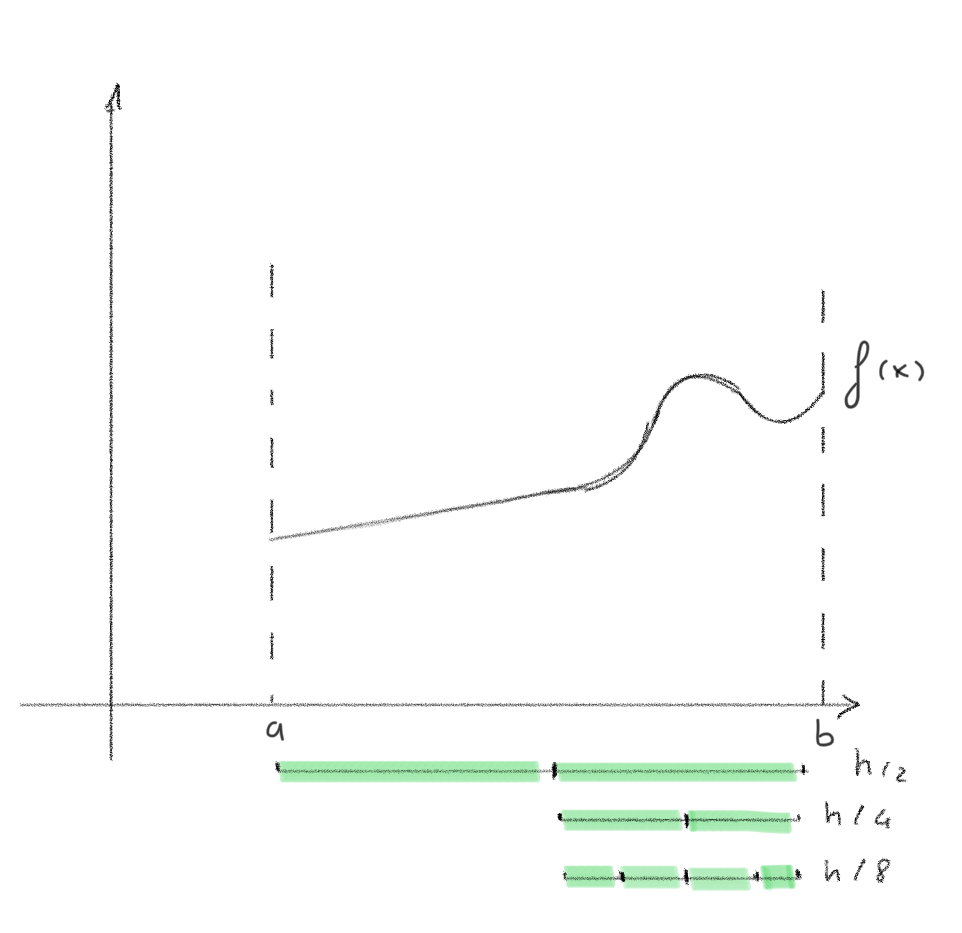
\includegraphics[width=0.5\linewidth]{adaptive}
    \caption{Metodo adattivo con controllo dell'errore che ci permette di
    calcolare il valore approssimato dell'integrale della funzione alla
tolleranza fissata suddividendo solo dove serve}
\end{figure}
\begin{lstlisting}[language=Python]
def trap_adapt(fn, a, b, fa, fb, tol, tab):
    m = 0.5 * (a + b)
    fm = fn(m)
    
    tam = trap_sing(a, m, fa, fm)
    tmb = trap_sing(m, b, fm, fb)
    
    if math.fabs(tab - tam - tmb) / 3 < tol:
        return (4 * (tam + tmb) - tab) / 3  # Estrapolazione di Richardson
    else:
        return (trap_adapt(fn, a, m, fa, fm, 0.5 * tol, tam) + 
                trap_adapt(fn, m, b, fm, fb, 0.5 * tol, tmb))
\end{lstlisting}
\paragraph{Caso Simpson.} 
Calcolando un Simpson con passo $h=\frac{b-a}{2}$ ($S(h)$) e
un Simpson con passo $h/2=\frac{b-a}{4}$ ($S(h/2)$); avremo la seguente
formula che fornisce un'approssimazione dell'integrale d'ordine
superiore:
$$ {\color{red}\left\lvert \displaystyle\int_{a}^{b}f(x) - S(h/2)\ dx\right\rvert
\approx \left\lvert \frac{1}{15}[S(h/2)-S(h)]\right\rvert}$$
da questa relazione, possiamo ottenere un'approssimazione migliore
dell'integrale come segue:
$${\color{green}\displaystyle\int_{a}^{b}f(x)\ dx\approx
\frac{1}{15}[16\cdot S(h/2)-S(h)]}$$
Utilizzando la {\color{red} prima relazione} possiamo implementare un
procedimento iterativo in cui il passo viene dimezzato fino a quando
la seguente condizione è soddisfatta: 
$$\left\lvert \frac{1}{15}[S(h/2)-S(h)]\leq tol\right\rvert$$
Una volta soddisfatta questa condizione, avremo che:
$$\left\lvert \displaystyle\int_{a}^{b}f(x)\ dx -
S(h/2)\right\rvert\leq tol$$
Di seguito il metodo adattivo per Simpson:
\begin{lstlisting}[language=Python]
def simp_adapt(fn, a, m, b, fa, fm, fb, tol, sab):
    m1 = 0.5*(a+m)
    m2 = 0.5*(m+b)
    fm1 = fn(m1)
    fm2 = fn(m2)
    sam = simp_sing(a, m, fa, fm1, fm)
    smb = simp_sing(m, b, fm, fm2, fb)
    
    if math.fabs(sab - sam - smb) / 15 < tol:
        return (16*(sam+smb) - sab)/15 # Estrapolazione di Richardson
    else:
        return (simp_adapt(fn, a, m1, m, fa, fm1, fm, 0.5*tol, sam) + 
                simp_adapt(fn, m, m2, b, fm, fm2, fb, 0.5*tol, smb)) 
\end{lstlisting}
\newpage
\section{Zeri di funzioni non lineari}
Si considera  il problema di trovare le radici di una funzione non
lineare, ovvero risolvere $f(x)=0$. 
Geometricamente, questo equivale a trovare i punti in cui la funzione $f(x)$
interseca l'asse delle ascisse (gli zero della funzione). 

\begin{center}
    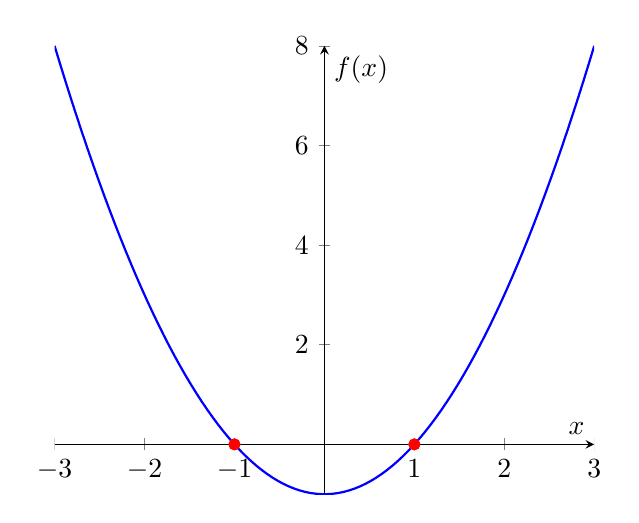
\begin{tikzpicture}
        \begin{axis}[
            axis lines = middle,
            xlabel = \(x\),
            ylabel = {\(f(x)\)},
            samples = 100,
            domain = -3:3,
            ]
            \addplot[blue, thick] {x^2 - 1};
            \addplot[only marks, red] coordinates {(-1, 0) (1, 0)};
        \end{axis}
    \end{tikzpicture} 
\end{center}

Per equazioni con grado $n\leq 4$, esistono soluzioni analitiche che
permettono di determinare le radici in modo esatto. Tuttavia, per equazioni di
grado superiore, non esistono soluzioni analitiche esplicite.

In questi casi, si ricorre a metodi numerici per approssimare le radici della
funzione.
\subsection{Metodo di bisezione}
Per poter applicare questo metodo la funzione $f(x)$ con $x\in[a,b]$ deve
rispettare le seguenti condizioni:
\begin{enumerate}
    \item \textbf{Continuità della funzione}: la funzione $f(x)$ deve essere
        continua nell'intervallo.
        $$f\in C[a,b]$$
    \item \textbf{Segno opposto agli estremi}: la funzione deve avere segni
        opposti agli estremi dell'intervallo $a$ e $b$.
        $$f(a)\cdot f(b)<0$$
\end{enumerate}
Se entrambe queste condizioni sono soddisfatte, allora esiste almeno un valore
$z$ nell'intervallo $(a,b)$ per cui $f(z)=0$.

Il metodo procede suddividendo ripetutamente l'intervallo $[a,b]$ a metà,
calcolando il punto medio $m$. Successivamente, si verifica quale dei due
nuovi intervalli $[a,m]$ o $[m,b]$ soddisfa la condizione per contenere $x^*$.
In particolare, se $f(a)f(m)<0$ allora $x^*\in[a,m]$; altrimenti
$x^*\in[m,b]$. L'intervallo scelto diventa il nuovo $[a,b]$, creando una
successione di intervalli $[a_k, b_k]$ per $k=1,\ldots,m$. Il procedimento
viene iterato sull'intervallo che è risultato contenere $x^*$ e viene
arrestato quando l'ampiezza dell'intervallo in esame risulterà minore di una
prefissata tolleranza $tol$.

\begin{center}
    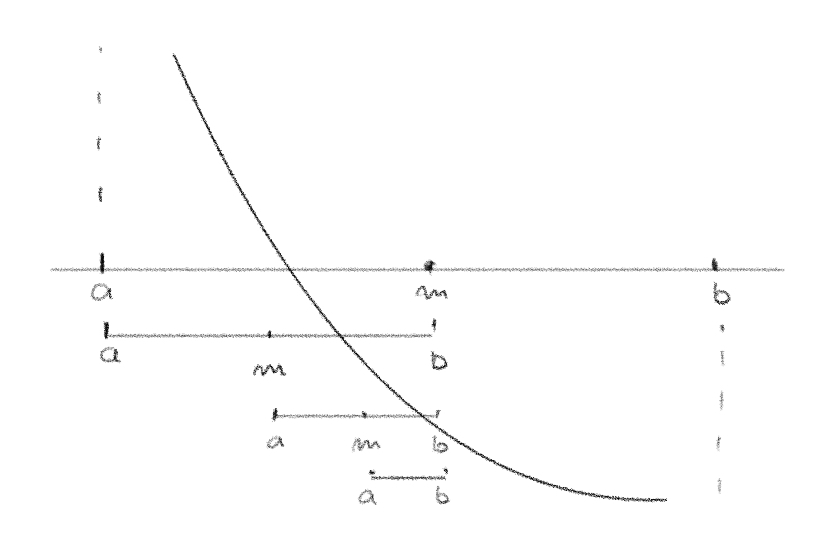
\includegraphics[width=0.5\linewidth]{bisection}
\end{center}
\begin{oss}\leavevmode\\
    Il valore di $tol$ non può essere scelto arbitrariamente piccolo, poiché 
    lavorando con numeri finiti la condizione di arresto
    $$\frac{\left\lvert b_k-a_k\right\rvert}{\min(\left\lvert
    a_k\right\rvert, \left\lvert b_k\right\rvert)}<tol$$
    potrebbe non essere mai soddisfatta. Poiché $a_k$ e $b_k$ sono numeri
    finiti, la loro distanza non sarà mai esattamente zero. Se la tolleranza
    $tol$ viene impostata a un valore minore della distanza tra $a_k$ e $b_k$
    il metodo potrebbe non convergere. 

    Si può dimostrare che la distanza relativa tra due numeri finiti
    consecutivi $X$ e $Y$ è data da 
    $$\frac{Y-X}{X}=2u$$
    Ne consegue che $tol$ deve essere maggiore di $2u$.

    Per evitare la divisione per zero quando $a_k$ o $b_k$ sono uguali a zero,
    il test di arresto può essere riformulato come segue:
    $$\left\lvert b_k-a_k\right\rvert < 2u\cdot \min(\left\lvert
    a_k\right\rvert,\left\lvert b_k\right\rvert)+tol$$
    dove ora $tol$ può essere scelto arbitrariamente e il problema della
    divisione per zero è evitato.
\end{oss}
\begin{oss}
    Se $x^*\equiv 0$ sarà sempre $a_k<0$ e $b_k>0$ per cui 
    $$\frac{\left\lvert b_k-a_k\right\rvert}{\min(\left\lvert
    a_k\right\rvert,\left\lvert b_k\right\rvert)}>1$$
    per evitare questo caso basta controllare se $f(0)\equiv 0$ quando
    $a<0<b$.
\end{oss}
\begin{lstlisting}[language=Python]
def bisez(fn, a, b, tol):
    if a<0 and b>0 and fn(0) == 0:
        return 0
    while abs(b-a) > 2*u*(min(abs(a), abs(b)))+tol:
        m = (a+b) / 2
        fm = fn(m)
        if fn(a)*fm < 0:
            b=m
        else:
            a=m
    return (a+b)/2 
\end{lstlisting}
Tuttavia, il metodo di bisezione presenta lo svantaggio di essere lento. In
particolare, ad ogni iterazione, l'approssimazione della radice migliora
soltanto di un bit. Considerando una precisione di tipo double, che dispone di una
mantissa di 53 cifre, sarebbero necessarie 53 iterazione per raggiungere
l'approssimazione desiderata della radice. 

Il problema del metodo di bisezione è che utilizza solo una frazione delle
informazioni disponibili. Nello specifico, si limita a considerare solamente
il segno della funzione agli estremi dell'intervallo in esame. Fortunatamente,
esistono metodi che superano questa limitazione, sfruttando informazioni
addizionali come il valore effettivo della funzione agli estremi, per
accelerare il processo di convergenza.
\subsubsection{Metodo della falsa posizione}
\begin{wrapfigure}{r}{0.4\textwidth}
    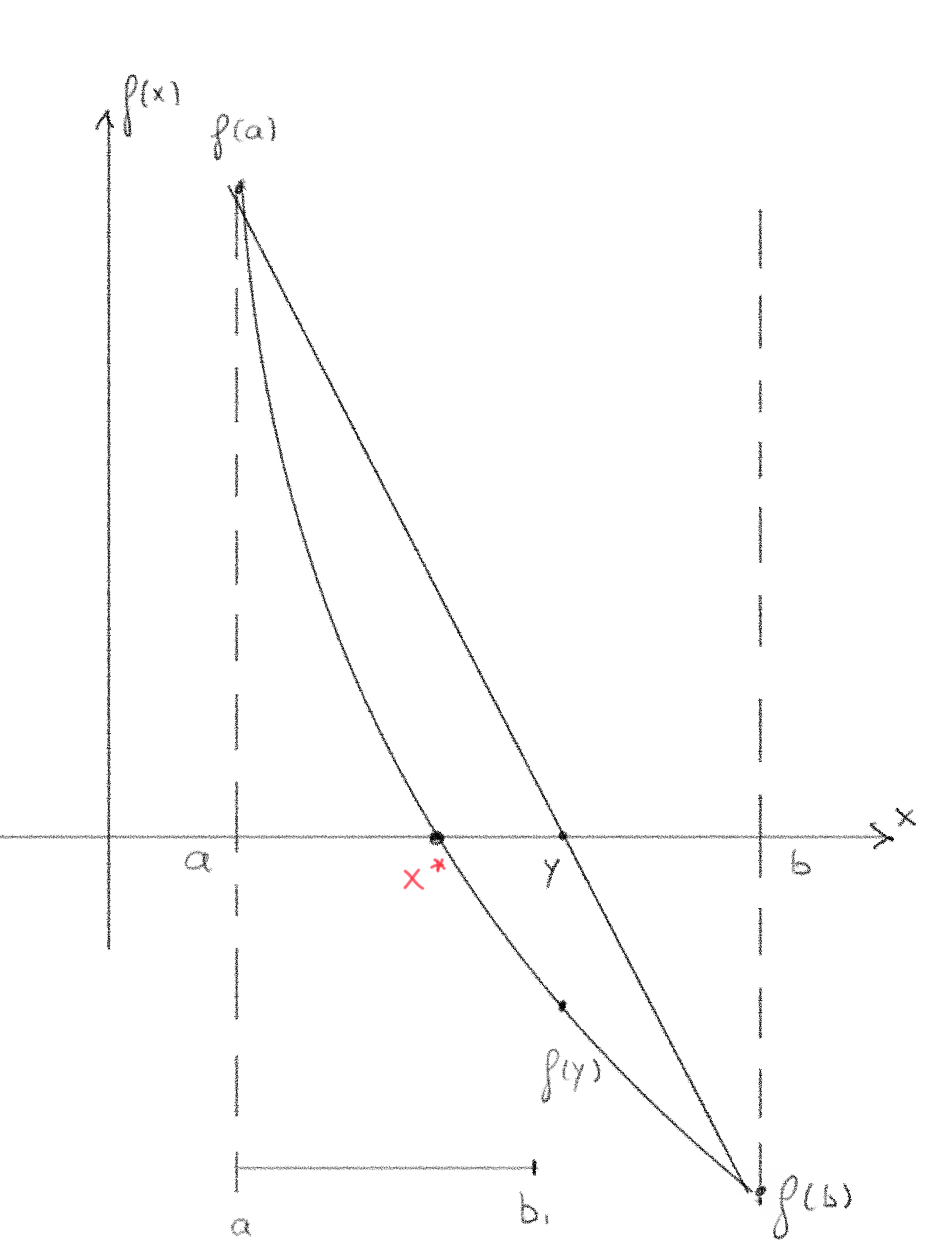
\includegraphics[width=0.9\linewidth]{false_position}
\end{wrapfigure}
Nel metodo della falsa posizione, si interpola una retta tra i punti $(a,f(a))$
e $(b,f(b))$ e si trova il punto $y$ in cui questa retta interseca l'asse $x$
tramite la formula:
$$y=b-\frac{f(b)(b-a)}{f(b)-f(a)}$$
Successivamente, si verifica quale dei due nuovi intervalli, $[a,y]$ o
$[y,b]$, soddisfa la condizione per contenere $x*$. Si sostituisce uno degli
estremi con $y$ e si continua iterativamente.

A differenza del metodo di bisezione, non stiamo rimpicciolendo gli intervalli
ma abbiamo che uno dei due estremi si avvicina sempre di più alla soluzione
$x^*$. Formalmente, avremo una successione $x_k$ con $k=0,\ldots,n$ di estremi
tale che:
$$x_k\underset{k\to\infty}{\to} x^*$$
Il test d'arresto delle falsi posizioni è diverso da quello del metodo della
bisezione. Si calcola la differenza relativa tra due iterative successive $x_k$ e
$x_{k-1}$ e confrontarla con la tolleranza desiderata:
$$\frac{\left\lvert x_k-x_{k-1}\right\rvert}{\min(\left\lvert
x_{k-1}\right\rvert, \left\lvert x_k\right\rvert)} < tol$$
e, come prima: 
$$\left\lvert x_k-x_{k-1}\right\rvert<2u\cdot\min(\left\lvert x_k\right\rvert,
\left\lvert x_{k-1}\right\rvert)+tol$$
Quindi, il metodo converge in molti meno passi rispetto al metodo di
bisezione.
\newpage
\begin{lstlisting}[language=Python]
def false_position(fn, a, b, tol):
    prev_y = None
    fa = fn(a)
    fb = fn(b)
    while True:
        y = b - (fb * (b - a)) / (fb - fa)
        if prev_y is not None and abs(y-prev_y) < 2*u*(min(abs(y),abs(prev_y)))+tol:
            return y
        fy = fn(y)
        if fa*fy < 0:
            b=y
            fb=fy
        else:
            a=y
            fa=fy
        prev_y = y
\end{lstlisting}
\subsection{Metodo di Newton}
Supponiamo di avere una funzione $f\in C^2[a,b]$ e di conoscere un punto $\bar{x}\in[a,b]$ che
sia un'approssimazione della soluzione $x^*$ tale che $f'(\bar{x})\neq 0$ e
che $\left\lvert \bar{x}-x^*\right\rvert$ sia piccolo.

Partiamo da uno sviluppo di Taylor centrato in $\bar{x}$:
$$f(x)=f(\bar{x})+f'(\bar{x})(x-\bar{x})+f''(\bar{x})\left(\frac{x-\bar{x}}{2}\right)^2+\ldots$$
Valutiamo $x^*$, usando lo sviluppo di Taylor:
$$\underbrace{f(x^*)}_{0}=f(\bar{x})+f'(\bar{x})(x^*-\bar{x})+f''(\bar{x})\left(\frac{x^*-\bar{x}}{2}\right)$$
Poiché $\left\lvert \bar{x} - x^*\right\rvert$ si è assunto piccolo,
$(x^*-\bar{x})^2$ sarà ancora più piccolo e ancora di più i termini
successivi; trascurando allora i termini non lineari abbiamo:
$$0=f(\bar{x})+f'(\bar{x})(x^*-\bar{x})$$
Risolvendo per $x^*$ otteniamo: 
$${\color{red}x^*-\frac{f(\bar{x})}{f'(\bar{x})}}$$
Questa relazione fornisce l'idea per il \textbf{metodo di Newton}, che
consiste nel generare una successione $\left\{x_k\right\}$ definita da:
\begin{equation}
    \begin{aligned}
        & x_{k+1}=x_k-\frac{f(x_k)}{f'(x_k)} &\text{con } k\geq0\text{ e
        }f'(x_k)\neq0\ \forall k.
    \end{aligned}
\end{equation}
Geometricamente, indica che ogni nuovo iterato $x_{k+1}$ è dato
dall'intersezione fra la retta tangente $f'(x_k)$,  alla $y=f(x_k)$ nel punto $x_k$ 
e l'asse $x$.

\begin{figure}[ht]
    \centering
    \begin{tikzpicture}[scale=1]
        \begin{axis}[
            axis lines = middle,
            xlabel = \( x \),
            ylabel = \( f(x) \),
            domain = 0:5,
            ymax = 10,
            xtick=\empty,
            ytick=\empty,
            samples = 100,
            ]
            \addplot[black, thick, no marks] {x^2 - 4};
            \addplot[blue, domain=1:4] {2*3*(x - 3) + (3)^2 - 4};

            \addplot[red, mark = *, only marks] coordinates {(3, 5) (2.166666, 0)};

            \node[below] at (axis cs: 3, 0) { \( x_k \) };
            \node[below] at (axis cs: 2.166666, 0) { \( x_{k+1} \) };
        \end{axis}
    \end{tikzpicture}
    \caption{Iterazione del metodo di Newton}
\end{figure}

Per verificare la convergenza della successione
$\left\{x_k\right\}_{k=0,1,\ldots}$, consideriamo una famiglia più generale di
metodi, di cui il metodo di Newton è un caso particolare. Questa famiglia di
metodi è nota come metodi di iterazione funzionale e sono descritti dalla
seguente formula
\begin{equation}\label{eq:metodo_iterazione_funzionale}
  \begin{aligned}
      & x_{k+1}=g(x_k) & k=0,1,\ldots
  \end{aligned}  
\end{equation}
Tali metodi risolvono un problema diverso: trovare le soluzioni dell'equazione 
$$x=g(x)$$
\begin{center}
    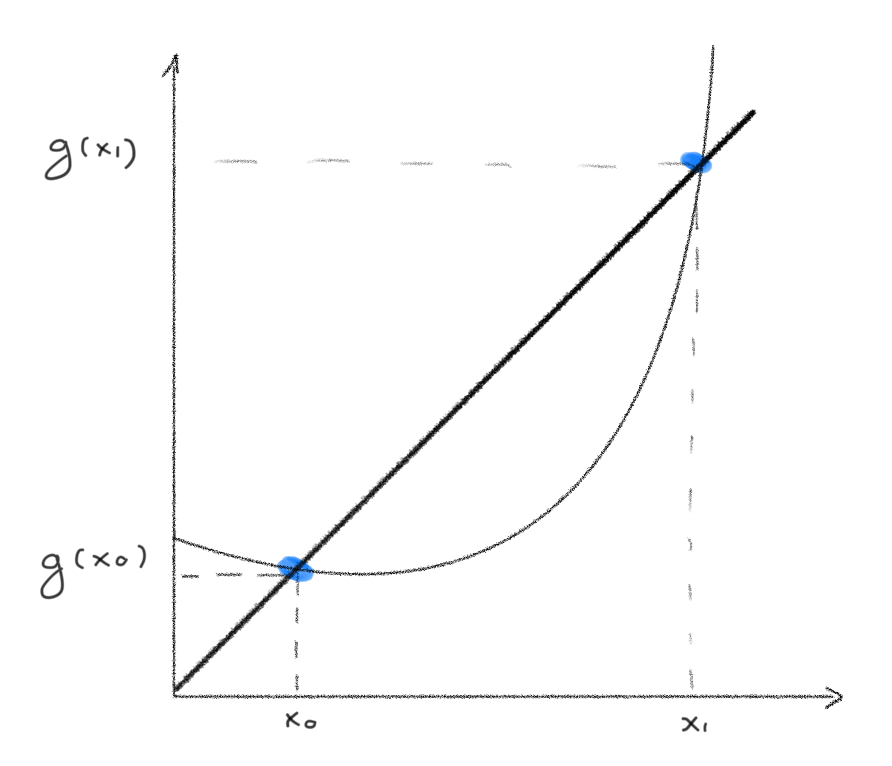
\includegraphics[width=0.5\linewidth]{functional_iteration}
\end{center}
Ciò significa trovare i punti di intersezione tra la retta bisettrice $y=x$ e
la curva $y=g(x)$. Questi sono detti \textbf{punti fissi} di $g(x)$, cioè i punti in cui la funzione
assume lo stesso valore dell'argomento.

Se $g(x)=x-\frac{f(x)}{h(x)}$ con $h(x)\neq0$, allora i due problemi sono
equivalenti e le radici di $f(x)=0$ sono anche i punti fissi di $g(x)$ e
viceversa.
\begin{proof}\leavevmode\
    \begin{itemize}
        \item Sia $f(x^*)=0$. Allora abbiamo
            \begin{equation*}
               \begin{aligned}
                   g(x^*)&=x^*-\frac{\overbrace{f(x^*)}^0}{h(x^*)}\\ 
                         &=x^*
               \end{aligned} 
            \end{equation*}
            il che implica che $x^*$ è un punto fisso d $g(x)$.
        \item Viceversa, sia $x^*$ un punto fisso di $g(x)$. In tal caso, si
            ha 
            $$\cancel{g(x^*)}=\cancel{x^*}-\frac{f(x^*)}{h(x^*)}$$
            che semplificato diventa $0=f(x^*)$.
    \end{itemize}
\end{proof}
Dopo aver stabilito l'equivalenza tra i due problemi, procediamo a dimostrare
la convergenza di un metodo iterativo funzionale.
\begin{theorem}
   Se $g(x)$ possiede un punto fisso $x^*$ e se $g(x)$ è continua e derivabile
   in $[x^*-\rho,x^*+\rho]$ con $\rho>0$ e soddisfa la condizione 
   $$\left\lvert g'(x)\right\rvert\leq \lambda<1\quad \text{con
   }x\in[x^*-\rho,x^*+\rho]$$
   Allora per ogni $x_0\in[x^*-\rho,x^*+\rho]$, tutti i successivi $x_k$
   generati dalla \ref{eq:metodo_iterazione_funzionale} appartengono 
   a questo intervallo e la successione converge a $x^*$.
\end{theorem}
In altre parole, il teorema ci dice che se partiamo da un punto iniziale $x_0$
che appartiene all'intervallo che contiene $x^*$, allora tutti i punti $x_k$
iterati successivi rimarranno all'interno di questo intervallo e convergeranno
al punto $x^*$.
\begin{proof}\leavevmode\
    $$\left\lvert x_{k-1}-x^*\right\rvert<\left\lvert x_k-x^*\right\rvert$$
    L'obiettivo è dimostrare che se la successione soddisfa questa
    condizione per ogni $k$, allora necessariamente converge a $x^*$.

    Per farlo, riscriviamo nel seguente modo:
    \[
    \begin{aligned}
        \left\lvert x_{k+1}-x^*\right\rvert &= \left\lvert g(x_k) - g(x^*) \right\rvert
    \end{aligned}
    \]
    Dove abbiamo utilizzato il fatto che $x_{k+1} = g(x_k)$ e $x^* = g(x^*)$.

    Applicando il teorema del valor medio, otteniamo:
    \[
    \begin{aligned}
        &= \left\lvert g'(\xi_k)(x_k-x^*) \right\rvert, \quad \text{dove} \quad \xi_k \in (x^*, x_k)
    \end{aligned}
    \]
    Dato che per ipotesi $|g'(x)| < \lambda$ su un intervallo che contiene
    $x^*$, abbiamo:
    \[
    \begin{aligned}
        &\leq \lambda \left\lvert x_k - x^* \right\rvert, \quad \text{dove} \quad \lambda < 1
    \end{aligned}
    \]
    Iterando questa disuguaglianza, otteniamo:
    \[
    \begin{aligned}
        &\leq \lambda^{k} \left\lvert x_0 - x^* \right\rvert
    \end{aligned}
    \]
    Poiché $\lambda < 1$, possiamo concludere che:
    \[
    \begin{aligned}
        \lim_{k \to \infty} \left\lvert x_{k+1} - x^* \right\rvert \leq \lim_{k \to \infty} \lambda^{k} \left\lvert x_0 - x^* \right\rvert = 0
    \end{aligned}
    \]
    Pertanto, la successione converge a $x^*$.
\end{proof}

\begin{figure}[ht]
   \centering
   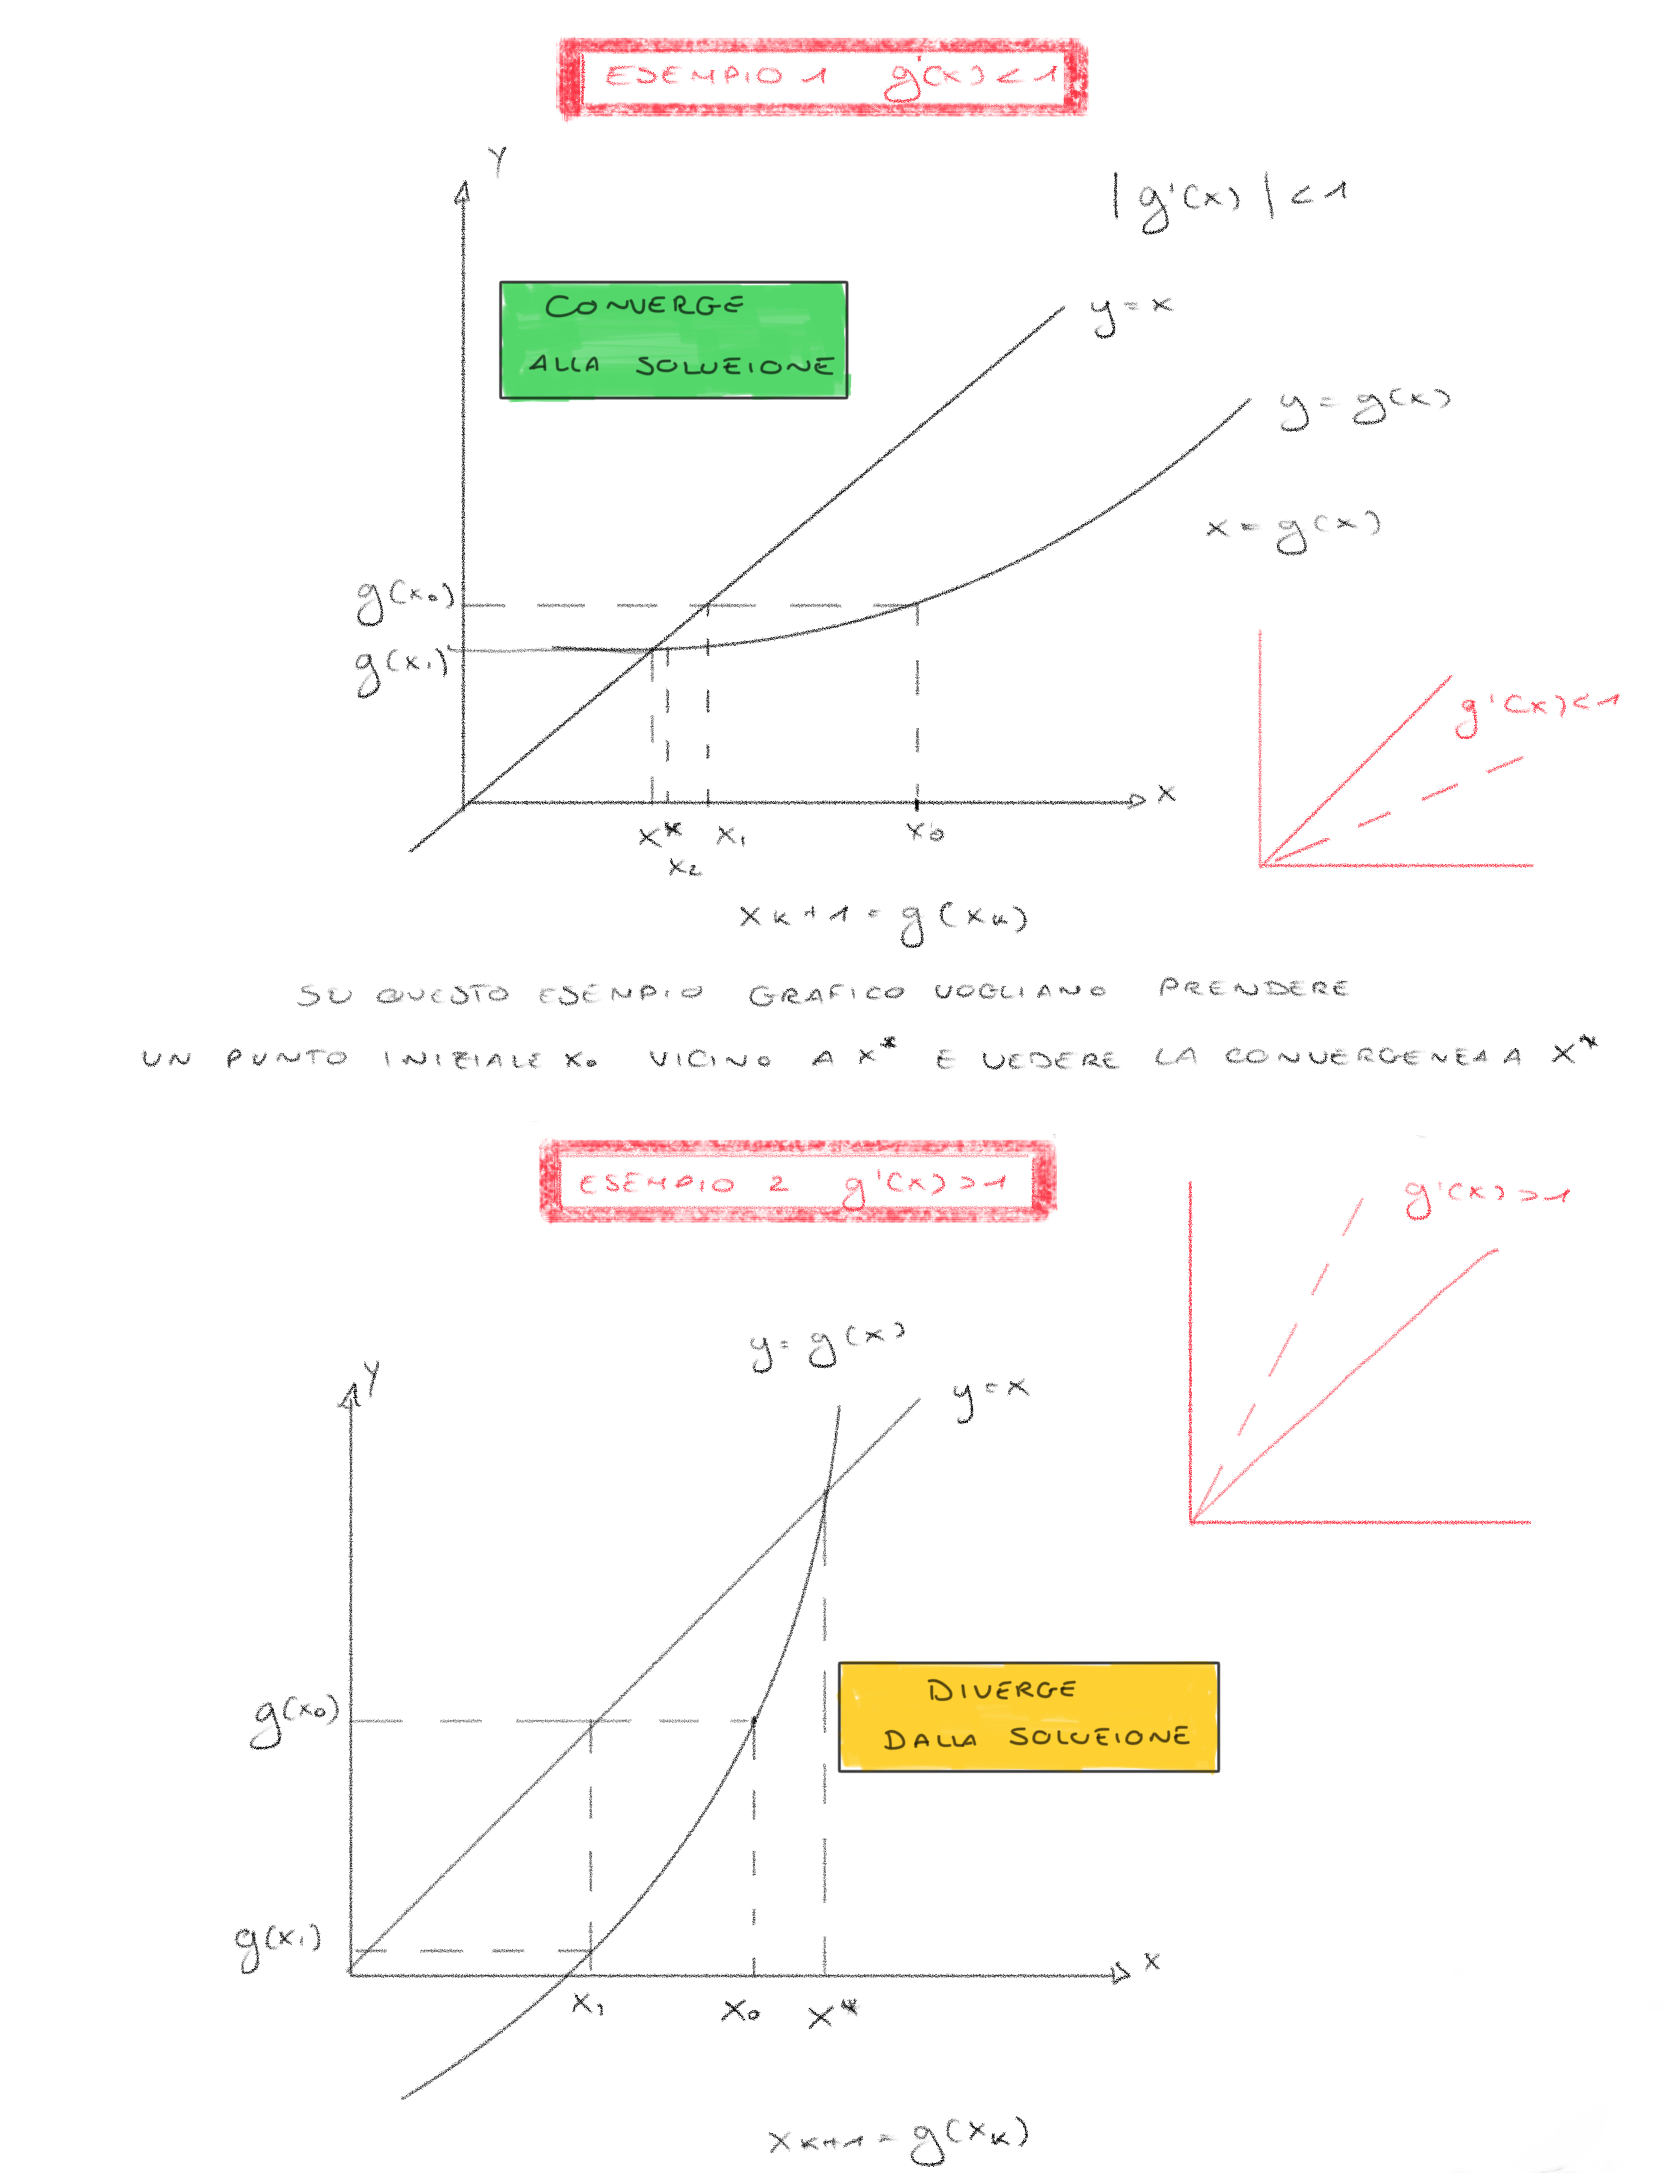
\includegraphics[width=0.8\linewidth]{example_iterative_method}
\end{figure}

Si vuole sfruttare il Teorema precedente per dimostrare il seguente risultato:

\begin{theorem}[Convergenza del metodo di Newton]
    Se $f(x)\in C^2[a,b]$, $f(x^*)=0$ e $f'(x^*)\neq0$, allora esiste un intervallo $I=[x^*-\rho,x^*+\rho]$ contenente
    $x^*$ tale che se $x_0\in I$ il metodo di Newton converge a  $x^*$.
\end{theorem}
\begin{proof}\leavevmode\
    Se scriviamo $g(x)=x-\frac{f(x)}{h(x)}$, con $h(x)\neq0$,
    le soluzioni di un problema sono le soluzioni dell'altro. Se prendiamo
    $h(x)=f'(x)$, otteniamo il metodo di Newton:
    $$g(x)=x-\frac{f(x)}{f'(x)}$$
    Il Teorema precedente afferma che la successione
    $x_{k+1}=g(x_k)$ converge a $x^*$ se $\left\lvert g'(x)\right\rvert<1$ per
    ogni $x\in I$. 

    Per verificare questa condizione, deriviamo $g(x)$ e otteniamo:
    \begin{equation*}
        \begin{aligned}
            g'(x)&=\cancel{1}-\cancel{\frac{[f'(x)]^2}{[f'(x)]^2}}+\frac{f''(x)f(x)}{[f'(x)]^2}
            \\ 
                 &=\frac{f''(x)f(x)}{[f'(x)]^2}
        \end{aligned}
    \end{equation*}
    Se valutiamo questa espressione in $x=x^*$, otteniamo:
    $$\frac{f''(x^*)f(x^*)}{[f'(x)]^2}$$
    Per ipotesi $f'(x^*)\neq0$ e $f(x^*)=0$ quindi l'espressione si annulla in
    $x^*$. Di conseguenza esiste un intorno di $x^*$ in cui $\left\lvert g'(x)\right\rvert<1$. 
    \begin{center}
        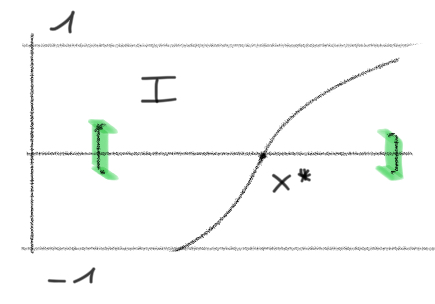
\includegraphics[width=0.25\linewidth]{newton_convergence}
    \end{center}
\end{proof}

Da ciò, possiamo concludere che la convergenza è garantita se, e solo
se, si seleziona un intervallo opportuno in cui $g'(x)<1$. Sotto queste
condizioni, il metodo convergerà sempre. Il passo successivo è quindi
determinare un intervallo $I$ attorno a $x^*$ che soddisfi questa condizione,
in modo da innescare con successo il metodo di Newton.

\paragraph{Test di arresto.} Nell'implementare il metodo di Newton, è bene
prevedere almeno tre test al verificarsi di uno dei quali ci si deve
arrestare:
\begin{enumerate}
    \item $|x_k-x_{k-1}|<2u\cdot\min(\left\lvert x_{k-1} \right\rvert,
        \left\lvert x_k\right\rvert)+tol$. Questo è analogo al test di arresto
        utilizzato nel metodo della falsa posizione.
    \item $k>max\_iter$. Se il valore iniziale $x_0$ non appartiene
        all'intervallo corretto, il metodo iterativo divergerà. In altre
        parole, gli iterati successivi non soddisfaranno mai il test di arresto,
        risultando in un ciclo infinito. Per prevenire questo problema,
        inseriamo un numero massimo di iterazioni, oltre al quale il metodo si
        arresterà.
    \item $\left\lvert f(x_k)\right\rvert\leq tol_{2}$. 
        L'errore inerente nel calcolo di uno zero $x^*$ di una
        funzione $f(x)$ è dato dalla formula: 
        $$\left\lvert \hat{x^*}-x^*\right\rvert=\frac{1}{f'(\xi)}E(\hat{x}^*)$$

        Questa equazione mostra che l'errore assoluto nel risultato dipende
        sia dall'errore nei dati $E(\hat{x}^*)$ e sia dal fattore che potrebbe
        amplificarlo , ovvero l'inverso della derivata prima $f'(\xi)$
        in un punto $\xi$ nell'intervallo $(x^*,\hat{x}^*)$.

        Osserviamo che se la derivata $f'(\xi)$ è molto piccola, il suo
        inverso sarà molto grande, e quindi anche un piccolo errore nei dati
        iniziali può essere amplificato in modo significativo. In tal caso, il
        problema è mal condizionato, e il metodo dovrebbe essere interrotto
        per evitare risultati inaccurati.
\end{enumerate}
\begin{lstlisting}[language=Python]
def newton(fn, fn_p, x0, tol):
    n=0
    max_iter=50
    small_real = 100*real_min
    
    x_curr = x0
    x_prev = x0 + 1
    while abs(x_curr - x_prev) > 2*u*min(abs(x_curr), abs(x_prev))+tol and n < max_iter:
        x_prev = x_curr
        fx_prev = fn(x_prev)
        if abs(fx_prev)>=small_real:
            x_curr = x_prev - (fx_prev / fn_p(x_prev))
            n=n+1
    return x_curr
\end{lstlisting}
\subsubsection*{Ordine di convergenza}
\begin{definition}
    Sia $\left\{x_k\right\}$ una successione convergente ad $x^*$ e sia
    $x_k\neq x^*$ $\forall k$. Se esiste un numero $p\geq 1$, tale
    che
    \begin{equation*}
       \begin{aligned}
           & \lim_{k\to\infty}\frac{\left\lvert e_{k+1}\right\rvert}{\left\lvert
   e_k\right\rvert^p}=\gamma & \text{dove } e_k=x_k-x^*
       \end{aligned} 
    \end{equation*}
    con 
    $$\begin{cases}
        0<\gamma\leq 1 & \text{se }p=1 \\
        \gamma>0 & \text{se }p>1
    \end{cases}$$
    si dice che la successione ha \textbf{ordine di convergenza} $p$. La
    costante $\gamma$ è detta \textbf{fattore di convergenza}.
    \begin{itemize}
        \item se $p=1$ e $0<\gamma<1$ si dice che la convergenza è
            \textbf{lineare};
        \item se $p=1$ e $\gamma=1$ si dice che la convergenza è
            \textbf{sublineare};
        \item se $p>1$ e $\gamma>0$ si dice che la convergenza è
            \textbf{superlineare}.
    \end{itemize}
\end{definition}
\begin{oss}
   Dalla definizione segue che esiste una costante $c$ tale che, da un certo
   $k$ in poi, si ha:
   $$\left\lvert e_{k+1}\right\rvert\leq c \left\lvert e_k\right\rvert^p$$
   Questa disuguaglianza misura la riduzione dell'errore assoluto ad ogni
   iterazione.
\end{oss}
\begin{example}
    Il metodo di bisezione
    $$\left\lvert e_{k+1}\right\rvert= \frac{1}{2}\left\lvert
    e_k\right\rvert^1$$
    ha un ordine di convergenza lineare.
\end{example}
\begin{theorem}
    Sia $\left\{x_k\right\}$ una successione generata da
    \ref{eq:metodo_iterazione_funzionale} convergente a $x^*$e sia $g(x)$
    sufficientemente regolare in un intorno di $x^*$. Allora la successione ha
    ordine di convergenza $p$ se e solo se 
    $$g'(x^*)=g''(x^*)=\ldots=g^{(p-1)}(x^*)=0,\quad g^{(p)}(x^*)\neq0$$
\end{theorem}
Per determinare l'ordine di convergenza di un metodo di iterazione funzionale,
si valuta $x^*$ in $g(x)$ e tutte le sue derivate successive. L'ordine di
convergenza $p$ è determinato da tutte le derivate nulle che precedono
l'ultima derivata non nulla $g^{(p)}(x^*)$.
\begin{oss}\leavevmode\\
    Poiché nel metodo di Newton abbiamo $g'(x^*)=0$, il metodo ha una
    convergenza pari a 2. 
\end{oss}

Questo vale solo nell'ipotesi che $f'(x^*)\neq0$, cioè se $x^*$ sia una radice
semplice di $f(x)$. Se invece la radice $x^*$ ha una molteplicità $m>1$,
l'ordine di convergenza non sarà più 2. Il metodo rimane tuttavia convergente,
ma con un ordine di convergenza ridotto a 1.
\begin{center}
    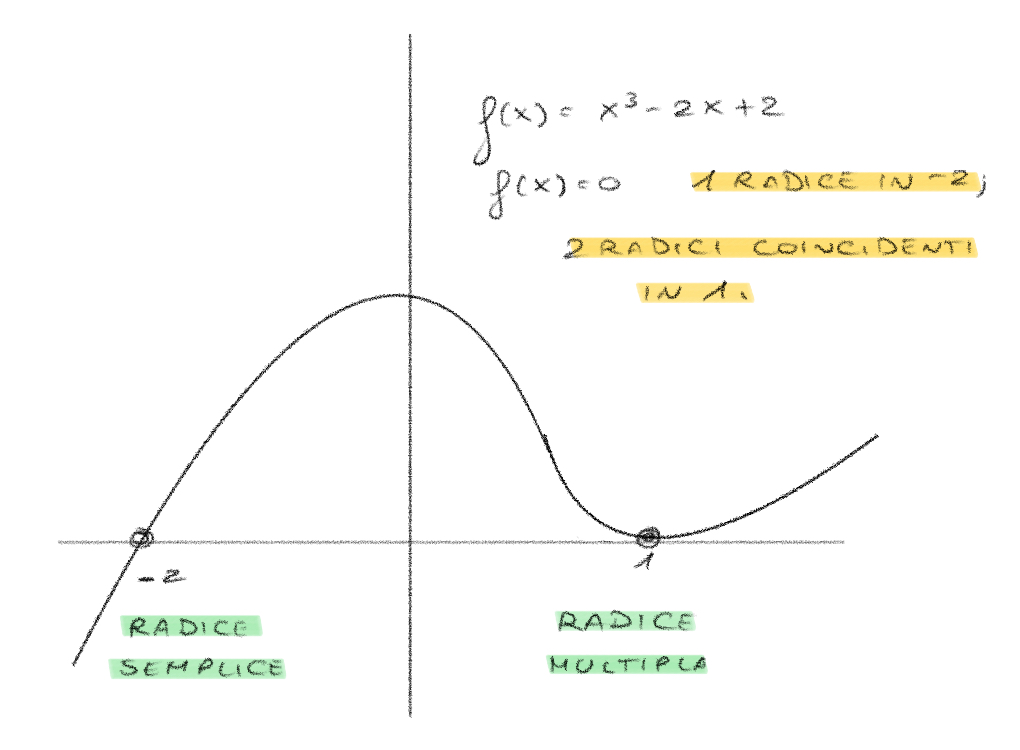
\includegraphics[width=0.5\linewidth]{newton_convergence_2}
\end{center}
\subsubsection{Metodo delle secanti}
Il metodo di Newton è veloce ma richiede di conoscere la derivata $f'(x)$
della funzione $f(x)$ che si sta esaminando. Quando la derivata è difficile da
calcolare o la sua valutazione è costosa, si può utilizzare il metodo delle
secanti come alternativa.

Nel metodo delle secanti, invece di utilizzare la retta tangente alla curva
della funzione in un punto $x_k$, si utilizza la retta secante che passa
attraverso due punti $(x_{k-1}, f(x_{k-1}))$ e $(x_k, f(x_k))$ sulla curva.
L'intersezione di questa retta con l'asse $x$ fornisce il prossimo iterato
$x_{k+1}$. ()

La formula per calcolare $x_{k+1}$ nel metodo delle secanti è:
$$x_{k+1}=x_k-\frac{f(x_k)}{f(x_k)-f(x_{k-1})}(x_k-x_{k-1})$$

Questa si può anche vedere considerando il metodo di Newton in cui alla
$f'(x_k)$ si sostituisce il rapporto incrementale.

\begin{theorem}
    Se $f(x)\in C^2[a,b],\ f(x^*)=0,\ f'(x^*)\neq0\text{ e }f''(x^*)\neq0$,
    allora esiste un intervallo $I=[x^*-\rho,x^*+\rho]$ tale che $x_0,x_1\in
    I$ ($x_0\neq x_1$) allora la successione $\left\{x_k\right\}$ (generata dal metodo delle
    secanti) converge a $x^*$ per $k\to\infty$.
    
    Inoltre, il 
    $$\lim_{k\to\infty}\frac{\left\lvert e_{k+1}\right\rvert}{\left\lvert
    e_k\right\rvert^p}=\gamma\neq0$$
    dove $p=\frac{1}{2}(\sqrt{5}+1)\approx1.618\ldots$
\end{theorem}

Il metodo delle secanti ha un ordine di convergenza che si colloca tra 1 e 2.
Questo lo rende  più efficiente di un algoritmo con convergenza lineare, ma
meno efficiente del metodo di Newton in termini di velocità di convergenza.

Tuttavia, c'è un aspetto da considerare: nel metodo delle secanti, il valore
$x_{k-1}$ è già stato calcolato nell'ite-razione precedente, quindi non è
necessario rivalutarlo. Al contrario, il metodo di Newton richiede la
valutazione sia della funzione che della sua derivata ad ogni iterazione.

In altre parole, sebbene il metodo di Newton possa convergere più rapidamente,
ogni sua iterazione è computazionalmente più costosa rispetto al metodo delle
secanti. Questo diventa particolarmente rilevante se la derivata della
funzione è onerosa da calcolare. In tali casi, il costo computazionale
associato al calcolo della derivata nel metodo di Newton potrebbe annullare i
vantaggi della sua più rapida convergenza.

\begin{lstlisting}[language=Python]
def secant(fn, x0, x1, tol):
    n=0
    max_iter=50
    small_real=100*real_min
    
    x_next = x1
    x_curr = x0
    fx_curr = fn(x0)
    while abs(x_next - x_curr) > 2*u*min(abs(x_next), abs(x_curr)) and n < max_iter:
        x_prev = x_curr
        fx_prev = fx_curr
        x_curr = x_next
        fx_curr = fn(x_curr)
        if (abs(fx_curr)>=small_real):
            x_next = x_curr - fx_curr * (x_curr-x_prev) / (fx_curr-fx_prev)
            n=n+1
    return x_next
\end{lstlisting}
\newpage
\section{Algebra lineare numerica}
\end{document}
